\documentclass{article}  % Define la clase del documento.

% Paquetes de idioma y codificación
\usepackage[utf8]{inputenc}
\usepackage[T1]{fontenc}
\usepackage[spanish]{babel}  % Ajusta el idioma del documento a español.
\addto\captionsspanish{
  \renewcommand{\figurename}{Figure}
  \renewcommand{\tablename}{Table}
}

\usepackage{tabularx}  % Permite la creación de tablas con ancho ajustable.

\usepackage{caption}
\usepackage{subcaption}

% Paquete de geometría para configurar márgenes y tamaño de papel
\usepackage[letterpaper, margin=3cm]{geometry}

% Paquetes de tipografía
\usepackage{mathptmx}    % Usa Times New Roman como fuente.
\usepackage{microtype}   % Mejora la justificación del texto.

% Paquetes para manejo de colores y gráficos
\usepackage{xcolor}      % Define y utiliza colores.
\usepackage{graphicx}    % Permite la inserción de imágenes.
\usepackage{tikz}        % Creación de gráficos vectoriales.

% Configuración de enlaces y referencias cruzadas
\usepackage{hyperref}
\hypersetup{
    colorlinks   = true,
    linkcolor    = darkblue,
    citecolor    = black,
    filecolor    = blue,
    urlcolor     = blue
}

\usepackage{media9} % Permite la inserción de multimedia.

% Paquetes para la mejora visual de tablas y figuras
\usepackage{booktabs}    % Para tablas de alta calidad.
\usepackage{float}       % Controla la posición de figuras y tablas.

% Paquete para la personalización de códigos fuente
\usepackage{listings}
\lstset{
    literate=
    {á}{{\'a}}1 {é}{{\'e}}1 {í}{{\'i}}1 {ó}{{\'o}}1 {ú}{{\'u}}1
    {Á}{{\'A}}1 {É}{{\'E}}1 {Í}{{\'I}}1 {Ó}{{\'O}}1 {Ú}{{\'U}}1
    {ñ}{{\~n}}1 {Ñ}{{\~N}}1 {ü}{{\"u}}1 {Ü}{{\"U}}1,
    backgroundcolor=\color{backcolour},
    commentstyle=\color{codegreen},
    keywordstyle=\color{codepurple},
    numberstyle=\tiny\color{codegray},
    stringstyle=\color{red},
    basicstyle=\ttfamily\small,
    breakatwhitespace=false,
    breaklines=true,
    captionpos=b,
    keepspaces=true,
    numbers=left,
    numbersep=5pt,
    showspaces=false,
    showstringspaces=false,
    showtabs=false,
    tabsize=2,
    language=TeX,
    morecomment=[l]\#,
    frame=single,
    rulecolor=\color{black}
}

% Definición de colores al estilo Visual Studio Code
\definecolor{darkblue}{rgb}{0.0, 0.0, 0.55}  % Enlaces
\definecolor{codegreen}{rgb}{0.25, 0.49, 0.48}  % Comentarios
\definecolor{codegray}{rgb}{0.5, 0.5, 0.5}  % Números y anotaciones
\definecolor{codepurple}{rgb}{0.58, 0, 0.82}  % Palabras clave
\definecolor{backcolour}{rgb}{0.95, 0.95, 0.92}  % Fondo de código

% Configuraciones de párrafo y matemáticas
\usepackage{amsmath}
\usepackage{parskip}    % Espaciado entre párrafos.
\usepackage{ragged2e}   % Justificación mejorada.
\usepackage{multicol}

% Configuración de secciones y encabezados
\usepackage{titlesec}
\titleclass{\part}{top} % Make part like a class
\titleformat{\part}[display]
  {\normalfont\huge\bfseries\centering}{\thepart}{40pt}{\Huge}
\titlespacing*{\part}{0pt}{-60pt}{10pt}
\titleformat{\part}
  {\normalfont\huge\bfseries}{}{0pt}{}

% Asegúrate de usar esto para mantener el estilo en las páginas de las partes
\titleformat{\part}[display]
  {\normalfont\huge\bfseries}{}{0pt}{}
  [\thispagestyle{fancy}] % Aplica el estilo fancy a las páginas de las partes

% Configuración de encabezados y pies de página personalizados
\usepackage{fancyhdr}
\pagestyle{fancy}
\fancyhf{}
\fancyhead[L]{\raisebox{0.20cm}{\textbf{Finite Elements - IOC5107}}}
\fancyhead[R]{\raisebox{0.1cm}{
\includegraphics[width=0.25\linewidth]{LOGO_UNIVERSIDAD.jpg}}}
\fancyhead[C]{\rule{\textwidth}{0.6pt}}
\fancyfoot[C]{\rule{\textwidth}{0.6pt}}
\fancyfoot[R]{\raisebox{-1.5\baselineskip}{\thepage}}
\renewcommand{\headrulewidth}{0pt}
\renewcommand{\footrulewidth}{0pt}

% Configuración avanzada de geometría
\geometry{
  top=3.5cm, % Aumenta el espacio en la parte superior para subir el encabezado
  bottom=2.5cm,
  headheight=2.5cm % Aumenta la altura del encabezado si es necesario
}

% Configuracion de bibliografia
\usepackage{natbib}
\bibliographystyle{unsrtnat}  % Puedes cambiarlo por `unsrtnat`, `abbrvnat`, etc.

\begin{document}
%----------------------------------------------------------------------------------------
% PORTADA
%----------------------------------------------------------------------------------------
\begin{titlepage}%Inicio de la carátula, solo modificar los datos necesarios
\newcommand{\HRule}{\rule{\linewidth}{0.5mm}} 
\center 
%----------------------------------------------------------------------------------------
%	ENCABEZADO
%----------------------------------------------------------------------------------------

\includegraphics[width=10cm]{LOGO_UNIVERSIDAD.jpg}\\ % Si esta plantilla se copio correctamente, va a llevar la imagen del logo de la facultad.OBS: Es necesario incluir el paquete: graphicx
\vspace{3cm}
%----------------------------------------------------------------------------------------
%	SECCION DEL TITULO
%----------------------------------------------------------------------------------------
\HRule \\[0.4cm]
{ \huge \bfseries Finite Elements - IOC5107}\\[0.4cm] % Titulo del documento
{ \huge \bfseries Final Report Homework 2}\\[0.4cm] % Titulo del documento
\HRule \\[1.5cm]
 \vspace{5cm}
%----------------------------------------------------------------------------------------
%	SECCION DEL AUTOR
%----------------------------------------------------------------------------------------
\begin{flushright}
  { \textbf{Profesor:}\\
  José Antonio Abell\\
  \textbf{Ayudante:}\\
  Nicolás Mora\\
  \textbf{Alumnos:} \\
  Felipe Vicencio\\
  Lukas Wolff\\
}
\end{flushright}
\vspace{1cm}
%----------------------------------------------------------------------------------------
%	SECCION DE LA FECHA
%----------------------------------------------------------------------------------------
{\large \textbf{\today}}\\[2cm] % El comando \today coloca la fecha del dia, y esto se actualiza con cada compilacion, en caso de querer tener una fecha estatica, reemplazar el \today por la fecha deseada
\end{titlepage}

\newpage
\thispagestyle{empty} % Deshabilita el número de página en la página del índice

%----------------------------------------------------------------------------------------
%  INDICE
%----------------------------------------------------------------------------------------
%\newpage
%\thispagestyle{empty} % Deshabilita el número de página en la página del índice
%\tableofcontents
%\thispagestyle{plain} % Deshabilita el encabezado en la página del índice
%\thispagestyle{empty} % Deshabilita el número de página en la página del índice
%\newpage

%\newpage
%\thispagestyle{empty}
%\listoffigures 
%\thispagestyle{plain} % Deshabilita el encabezado en la página del índice %
%\thispagestyle{empty}
\newpage
%----------------------------------------------------------------------------------------
%ACÁ EMPIEZA EL INFORME
\setcounter{page}{1}
%----------------------------------------------------------------------------------------

\section{Introduction}

Finite Element Analysis (FEA) is a numerical method for predicting the response of structures under loading conditions. By discretizing a continuous domain into smaller elements, the method allows to compute distributions of stress, strain, and displacement.

This report presents the structural analysis of a 3D-printed wrench using 2D triangular constant strain triangle (CST) elements under the plane stress assumption. The main objective is to investigate the mechanical behavior of the wrench under different loading scenarios, focusing on its deformation and internal stress/strain states.

Three cases are considered: (a) a total vertical load of 30 kgf applied as a distributed force, (b) the same load applied at a single node, and (c) a distributed load including the effect of self-weight. Each case includes graphs of the deformed shape, stress and strain components, principal values, and a discussion of mesh convergence and precision techniques.

The analysis also includes an optimization study to minimize the maximum principal tensile stress while maintaining constant material volume. The analysis was perfomed using a \textit{Python} program that implementes this methodology. For the mesh generation and optimization, the GMESH \textit{software} was used.

\newpage

\section{Theoretical background}

\subsection{Finite Element Method (FEM)}

The Finite Element Method (FEM) is a numerical technique used to solve complex engineering problems. It involves dividing a large system into smaller and simpler parts called finite elements. The behavior of each element is described by a set of equations, and the overall response of the system is obtained by assembling these equations. The method used in this report is the CST based model.

\subsection{CST elements}

The CST (Constant Strain Triangle) is a 2D, three-node finite element used for plane stress/strain problems.  
It assumes linear displacement fields, producing constant strain and stress within each element. The CST element is defined by three nodes, each with two degrees of freedom (DOF) corresponding to the in-plane displacements. The element stiffness matrix is derived from the shape functions and material properties, allowing for the calculation of nodal displacements and internal forces.

\subsection{Plane stress assumption}

This condition applies to thin structures where the stress components perpendicular to the plane are negligible. Mathematically, this means $\sigma_z = \tau_{xz} = \tau_{yz} = 0$. The dominant stress components are $\sigma_{xx}$, $\sigma_{yy}$, and $\sigma_{xy}$. This assumption is typically valid in thin plates or sheets subjected to in-plane loading and is commonly used in finite element analysis (FEA) with 2D CST elements under plane stress conditions.

\subsection{Plane strain assumption}

This assumption is used for long or thick bodies where deformation in one direction (usually the z-axis) is constrained. In this case, the strain components are $\varepsilon_z = \gamma_{xz} = \gamma_{yz} = 0$, although $\sigma_z$ can be non-zero. This is applicable to structures such as tunnels, dams, and thick-walled pressure vessels. All in-plane stress components remain active, and a different constitutive matrix $\mathbf{D}$ is used compared to the plane stress condition.

\subsection{Shape functions}

The shape functions are used to interpolate the displacements within the element based on the nodal displacements. For a CST element, the shape functions are defined as:

\begin{equation}
  N_i(\xi) = \begin{bmatrix}
  \xi_1 & 0 & \xi_2 & 0 & \xi_3 & 0 \\
  0 & \xi_1 & 0 & \xi_2 & 0 & \xi_3
  \end{bmatrix}
\end{equation}

Where $\xi_1$, $\xi_2$, and $\xi_3$ are the coordinates of the nodes in the local coordinate system. The shape functions are used to relate the nodal displacements to the displacements at any point within the element.
The shape functions are linear and can be expressed in terms of the local coordinates $\xi$ and $\eta$ as follows:
\begin{equation}
  N_1 = \frac{1}{2} (1 - \xi - \eta), \quad N_2 = \frac{1}{2} (1 + \xi), \quad N_3 = \frac{1}{2} (1 + \eta)
\end{equation}

\subsection{Strain displacement matrix}

The strain displacement matrix relates the nodal displacements to the interal deformation of the element. For a CST element, the strain-displacement matrix $\mathbf{B}$ is defined as:

\begin{equation}
  B = \begin{bmatrix}
  \frac{\partial \xi_1}{\partial x} & 0 & \frac{\partial \xi_2}{\partial x} & 0 & \frac{\partial \xi_3}{\partial x} & 0 \\
  0 & \frac{\partial \xi_1}{\partial y} & 0 & \frac{\partial \xi_2}{\partial y} & 0 & \frac{\partial \xi_3}{\partial y} \\
  \frac{\partial \xi_1}{\partial y} & \frac{\partial \xi_1}{\partial x} & \frac{\partial \xi_2}{\partial y} & \frac{\partial \xi_2}{\partial x} & \frac{\partial \xi_3}{\partial y} & \frac{\partial \xi_3}{\partial x}
  \end{bmatrix}
\end{equation}

This matrix derives the shape functions in order to obtain the internal strain components as follows:

\begin{equation}
  \begin{bmatrix}
  \varepsilon_x \\
  \varepsilon_y \\
  \gamma_{xy}
  \end{bmatrix} = \mathbf{B} \begin{bmatrix}
  u_1 \\
  u_2 \\
  u_3
  \end{bmatrix}
\end{equation}

Where $\varepsilon_x$ and $\varepsilon_y$ are the normal strains in the x and y directions, respectively, and $\gamma_{xy}$ is the shear strain. The vector of nodal displacements is represented by $u_1$, $u_2$, and $u_3$.

\subsection{Stiffness matrix}

The stiffness matrix is used to calculate the internal forces and displacements ot the element from the nodal displacements. 

\begin{equation}
  K^{(e)} = \int_{\Omega^{(e)}} B^T E B \, t \, d\Omega^{(e)}
\end{equation}

Where $K^{(e)}$ is the element stiffness matrix, $E$ is the material's elastic modulus, $t$ is the thickness of the element, and $\Omega^{(e)}$ is the area of the element. The stiffness matrix relates the nodal forces to the nodal displacements as follows:

\begin{equation}
  \mathbf{F} = \mathbf{K} \mathbf{u}
\end{equation}

\subsection{Nodal forces vector}

To obtain the nodal forces vector, a body force is applied (self-weight), then the nodal forces vector is calculated as follows:

\begin{equation}
  f^{(e)} = \int_{\Omega^{(e)}} t \left( N^{(e)} \right)^T b \, d\Omega^{(e)}
\end{equation}

Where $f^{(e)}$ is the nodal forces vector, $N^{(e)}$ is the shape function matrix, and $b$ is the body force vector. The nodal forces vector relates the body forces to the nodal displacements as follows:
\begin{equation}
  \mathbf{F} = \mathbf{K} \mathbf{u} + \mathbf{f}
\end{equation}

\subsection{Von Mises stress Criterion}

In structural analysis, the Von Mises stress is widley used as a yield and failure crtierion. The Von Mises stress is a scalar value derived from the stress components and provides a singles equivalent stress that can be directly compared to the material's yield strenght.
Under plane stress conditions, the Von Mises stress $\sigma_{VM}$ is calcultaed using the in-plane stresses as follows:

\begin{equation}
  \sigma_{VM} = \sqrt{ \sigma_{xx}^2 - \sigma_{xx} \sigma_{yy} + \sigma_{yy}^2 + 3\sigma_{xy}^2 }
\end{equation}
  

Where $\sigma_{xx}$ and $\sigma_{yy}$ are the normal stresses in the x and y directions, respectively, and $\tau_{xy}$ is the shear stress in the xy plane. 
\newpage

\section{Materials for the model}

For this asignment, a wrech was design using the GMESH \textit{software}. The wrench was designed to be 3D printed, and the material used was PLA. 

This material is a thermoplastic polymer that is widley used in 3D printing due to its mechanical properties. Moreover, depending on the printing orientation, fill density and extrusion temperature, the mechanical properties of PLA can vary significantly. For this analysis, the following properties were used:

\begin{itemize}
  \item Young's modulus: $3.5 \times 10^9 Pa$
  \item Poisson's ratio: 0.36
  \item Tensile Yield strength: $50 \times 10^6 Pa $
  \item Density: $1.252 \times 10^3 kg/m^3$
\end{itemize}

These values were chosen based on the standard levels used in other experiences. \citet{farah2016}

\newpage

\section{Description of the model}

The model for this assignment was a wrench designed using the GMESH \textit{software}. The purpose of this was to analyze the mechanical behavior of the structure under 3 different cases. 

The first case was a distributed load applied to one end of the wrench, as shown in Figure \ref{caso1}.

The second case was a point load applied to the same end of the first case. The variation from this case to the previous one is considerable, due to the force being adjusted to only one node instead to a list of nodes.

At last, the third case was similar to case 1, but with the addition of a self-weight load. This was done by adding a body force to the model in that same region.

\begin{figure}[H]
  \centering
  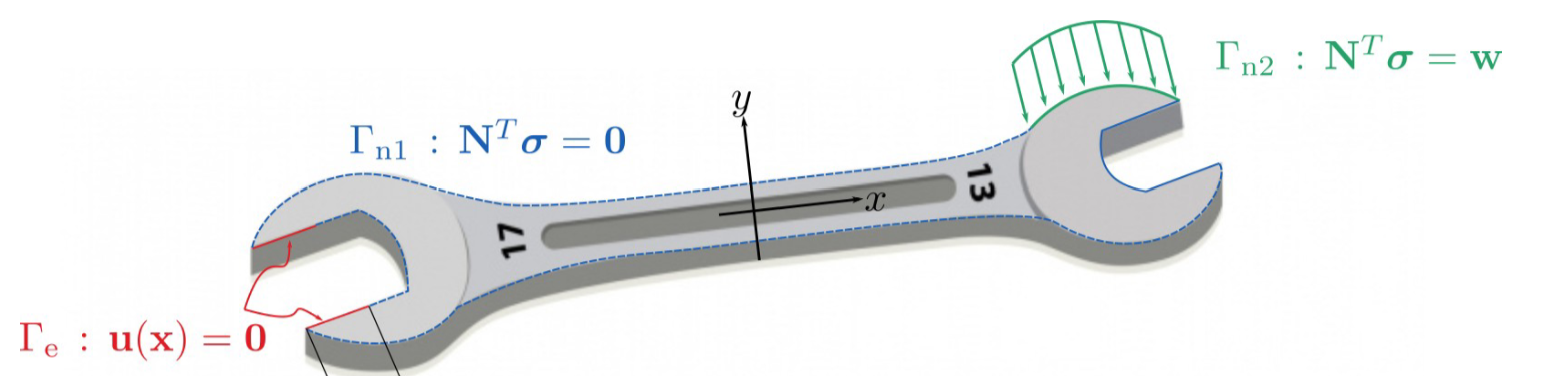
\includegraphics[width=0.8\textwidth]{img/wrench.png}
  \caption{Wrench model with limited boundaries and regions of particular behavior.}
  \label{caso1}
\end{figure}

\section{Results and Analysis}

This section presents the results obtained from the simulation of the proposed algorithm. The objective of this assignment was to evaluate and analyze the wrench behavior under 3 different cases presented below. It is worth noting that for the results to be precise and coherent, a convergence study was performed. This process ensure the accurasy and physical validity of the reuslts, resulting in a mesh size of about $l_c=0.8$.

\subsection{Case 1: Distributed load apllied to one end of the wrench}

For this case, a $30 kgf$ distributed load was applied at the wrench deforming it in the $y$ direction. This can be observed in Figure \ref{fig:stress}.

\begin{figure}[H]
    \centering
    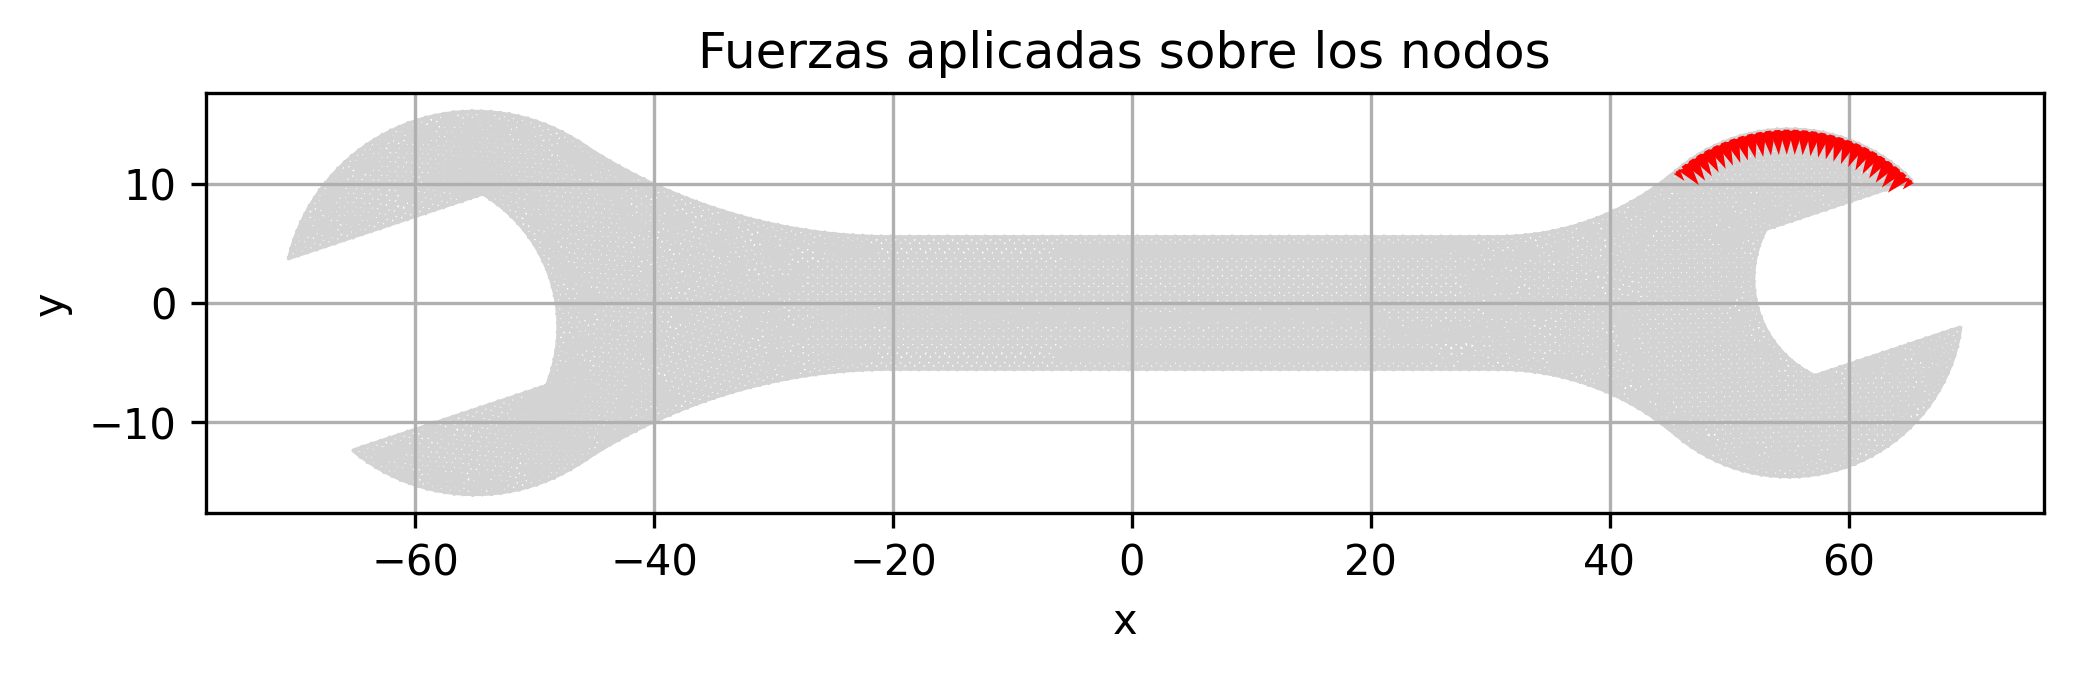
\includegraphics[width=0.8\textwidth]{GRAFICOS/Case b_fuerzas.png}
    \caption{Distributed load applied to the wrench}
    \label{fig:xd}
\end{figure}

\begin{figure}[H]
    \centering
    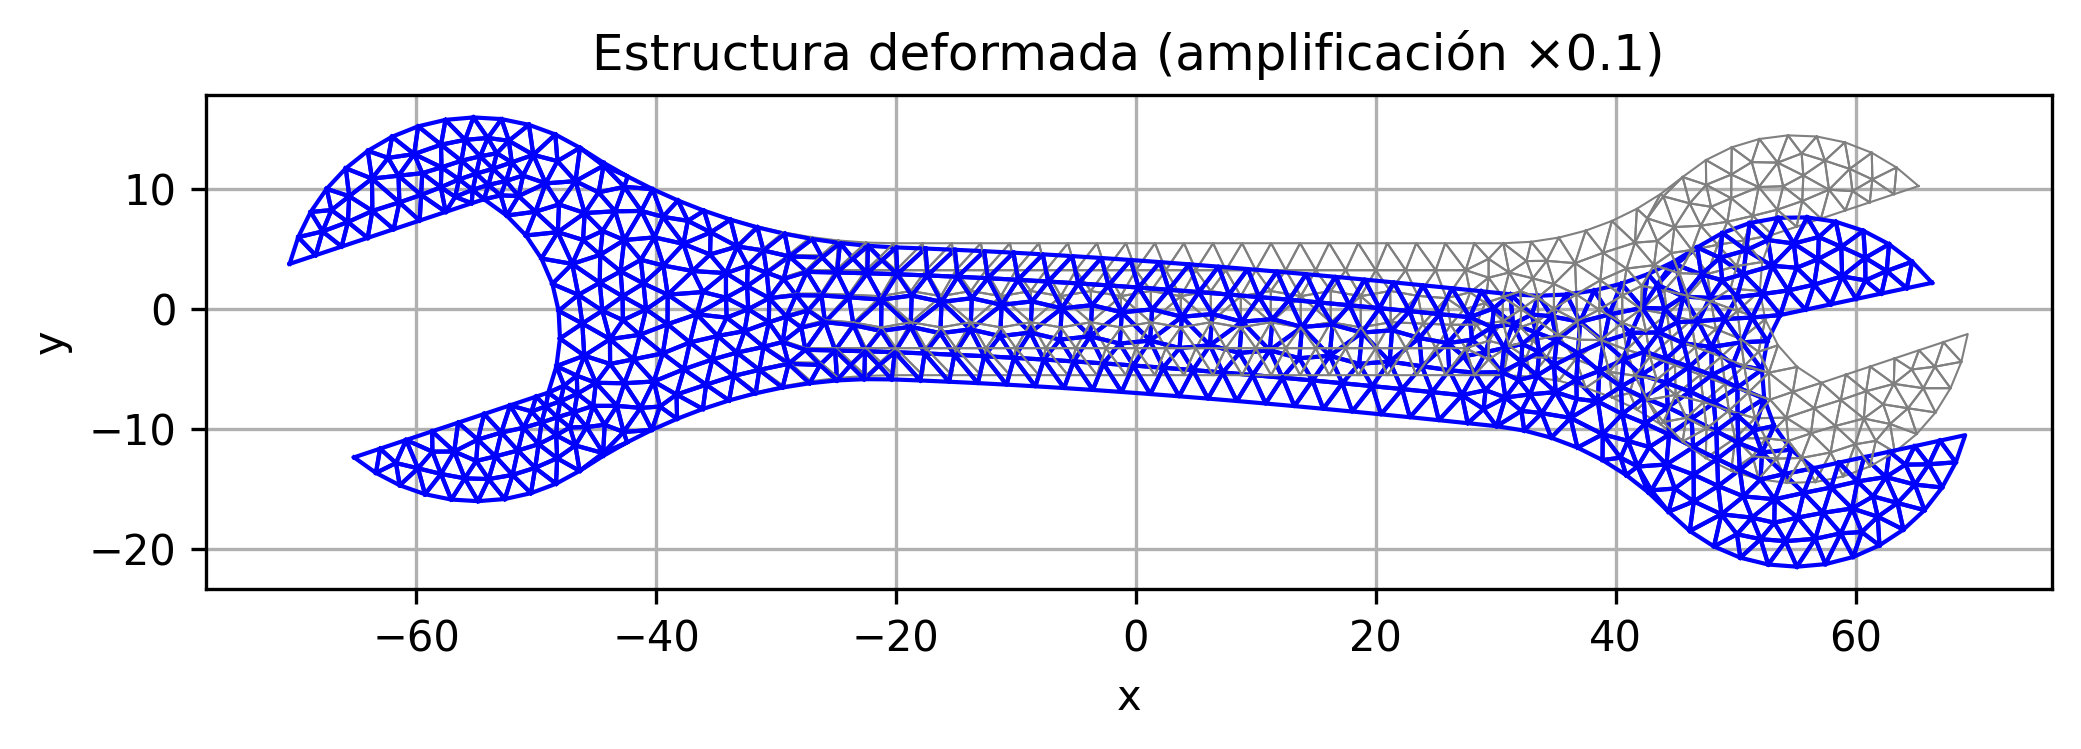
\includegraphics[width=0.8\textwidth]{GRAFICOS/Case b_deformada.png}
    \caption{Deformed wrench with distributed load}
    \label{fig:stress}
\end{figure}

The results of normal stresses, shear stresses, and displacements are shown below, as well as the principal stresses and strains.

\begin{table}[H]
    \centering
    \caption{Stress (Pa) and strain components}
    \begin{tabular}{|c|c|c|c|c|c|}
    \hline
    $\sigma_{xx}$ & $\sigma_{yy}$ & $\tau_{xy}$ & $\epsilon_{xx}$ & $\epsilon_{yy}$ & $\gamma_{xy}$ \\
    \hline
    360 & 60 & -60 & 0.09 & 0.036 & -0.05 \\
    \hline
    \end{tabular}
    \label{tab:tabla1}
\end{table}
    
\begin{table}[H]
    \centering
    \caption{Principal Stresses (Pa) and strain components}
    \begin{tabular}{|c|c|c|c|}
    \hline
    $\sigma_{1}$ & $\sigma_{2}$ & $\epsilon_{1}$ & $\epsilon_{2}$ \\
    \hline
    360 & -360 & 0.108 & -0.108 \\
    \hline
    \end{tabular}
    \label{tab:tabla2}
\end{table}

Finally, the Von Misses stress is plotted below, reaching a maximum value of $\sigma_{VM} = 360 Pa$.

\begin{figure}[H]
    \centering
    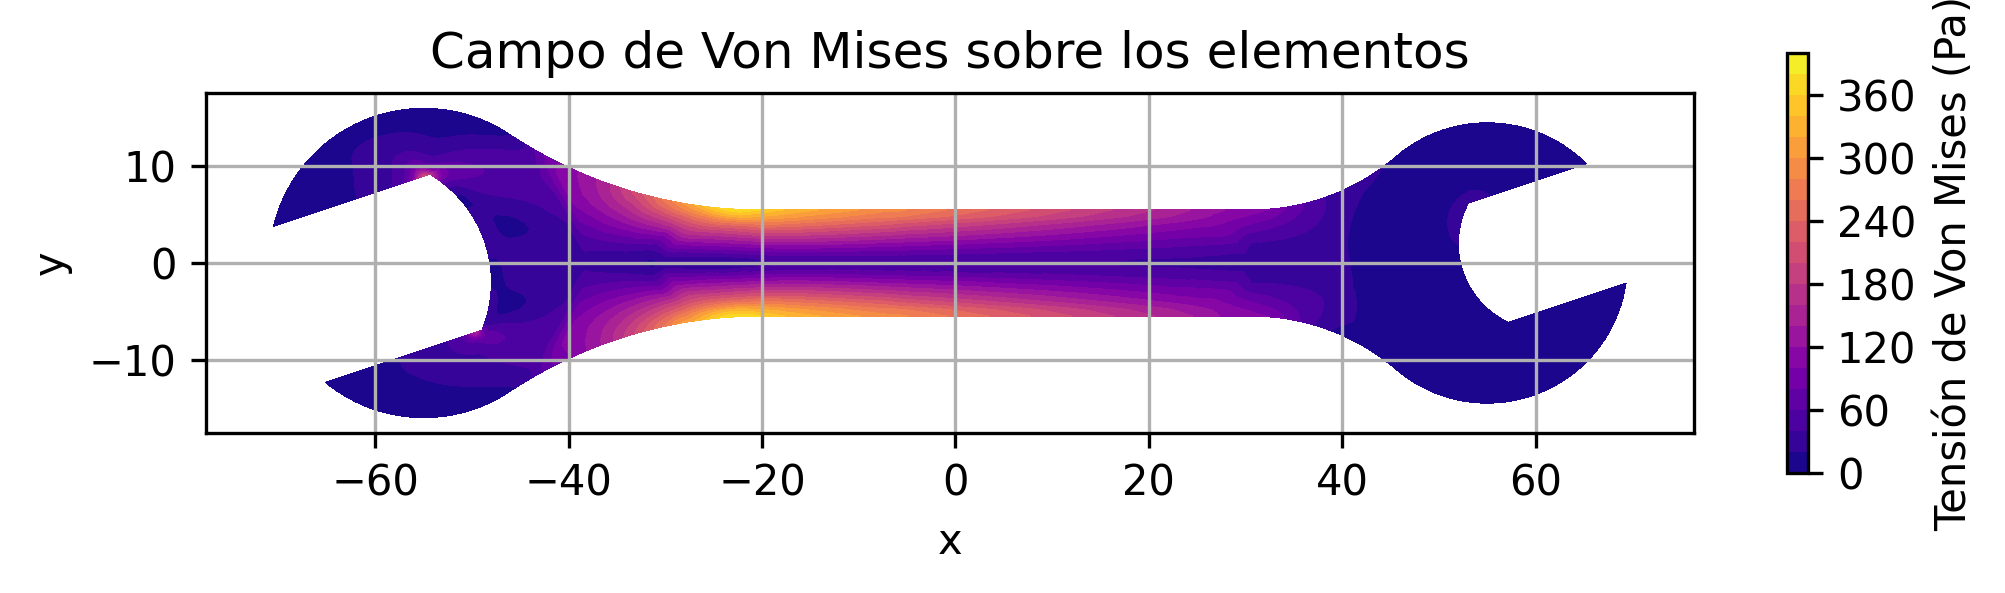
\includegraphics[width=0.8\textwidth]{GRAFICOS/Case b_von_mises.png}
    \caption{Von Misses stress distribution for the distributed load}
    \label{fig:principal}
\end{figure}

\subsection{Case 2: Point load applied to one end of the wrench}

Different to the previous case, a point load of $30 kgf$ was applied to one end of the wrench. This can be observed in Figure \ref{fig:xdd}. Also, the deformed state is shown in Figure \ref{fig:xdi}.

\begin{figure}[H]
    \centering
    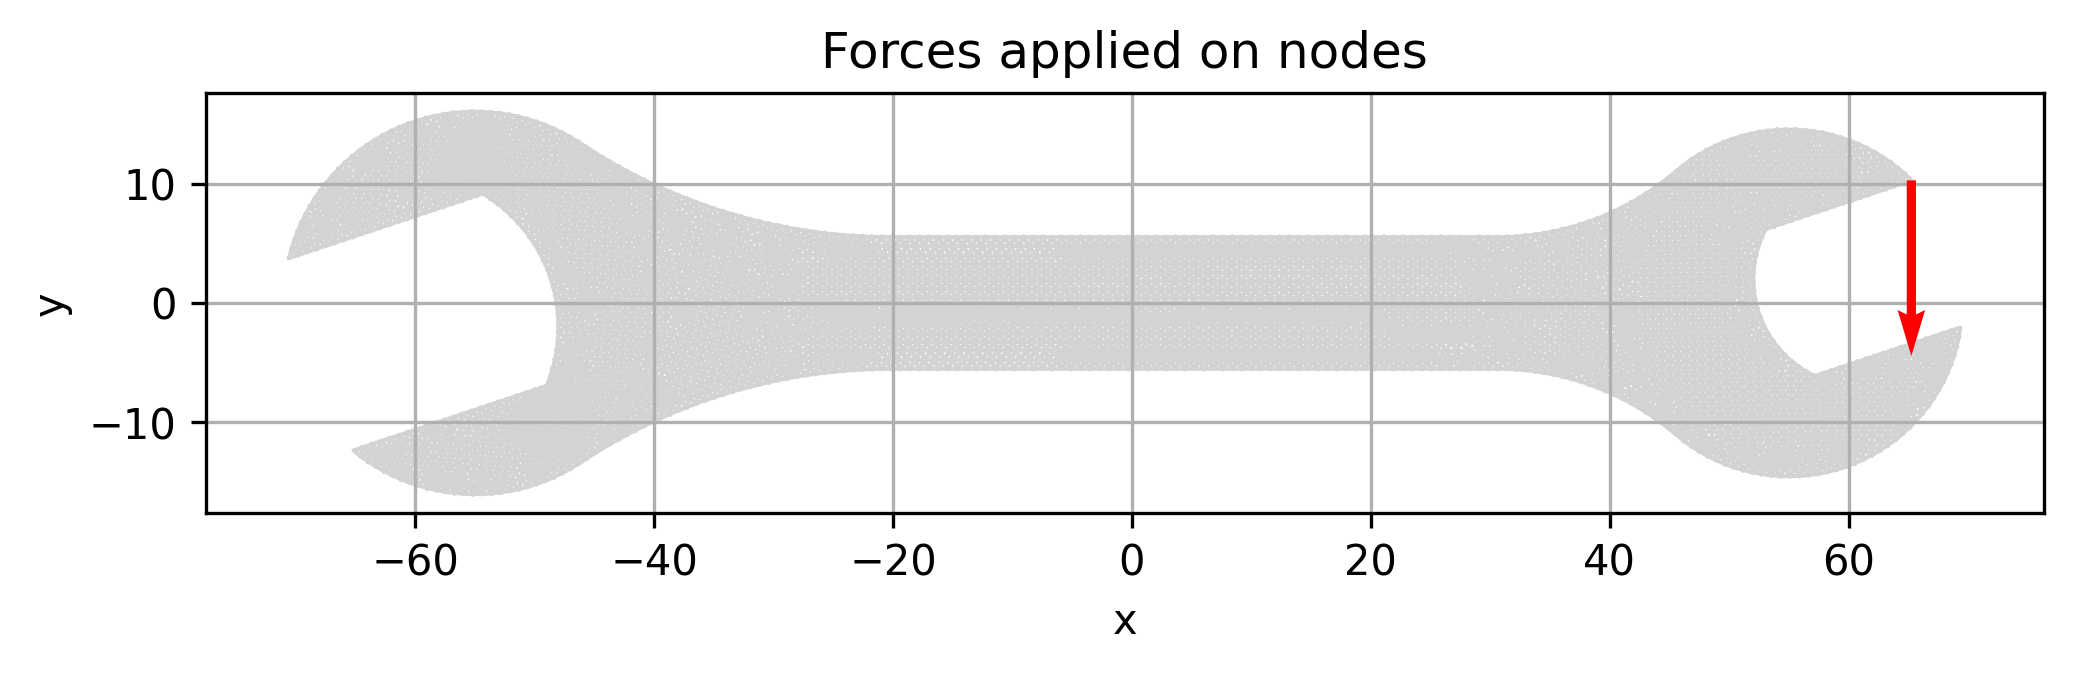
\includegraphics[width=0.8\textwidth]{GRAFICOS/Case a_fuerzas.png}
    \caption{Point load applied to the wrench}
    \label{fig:xdd}
\end{figure}

\begin{figure}[H]
    \centering
    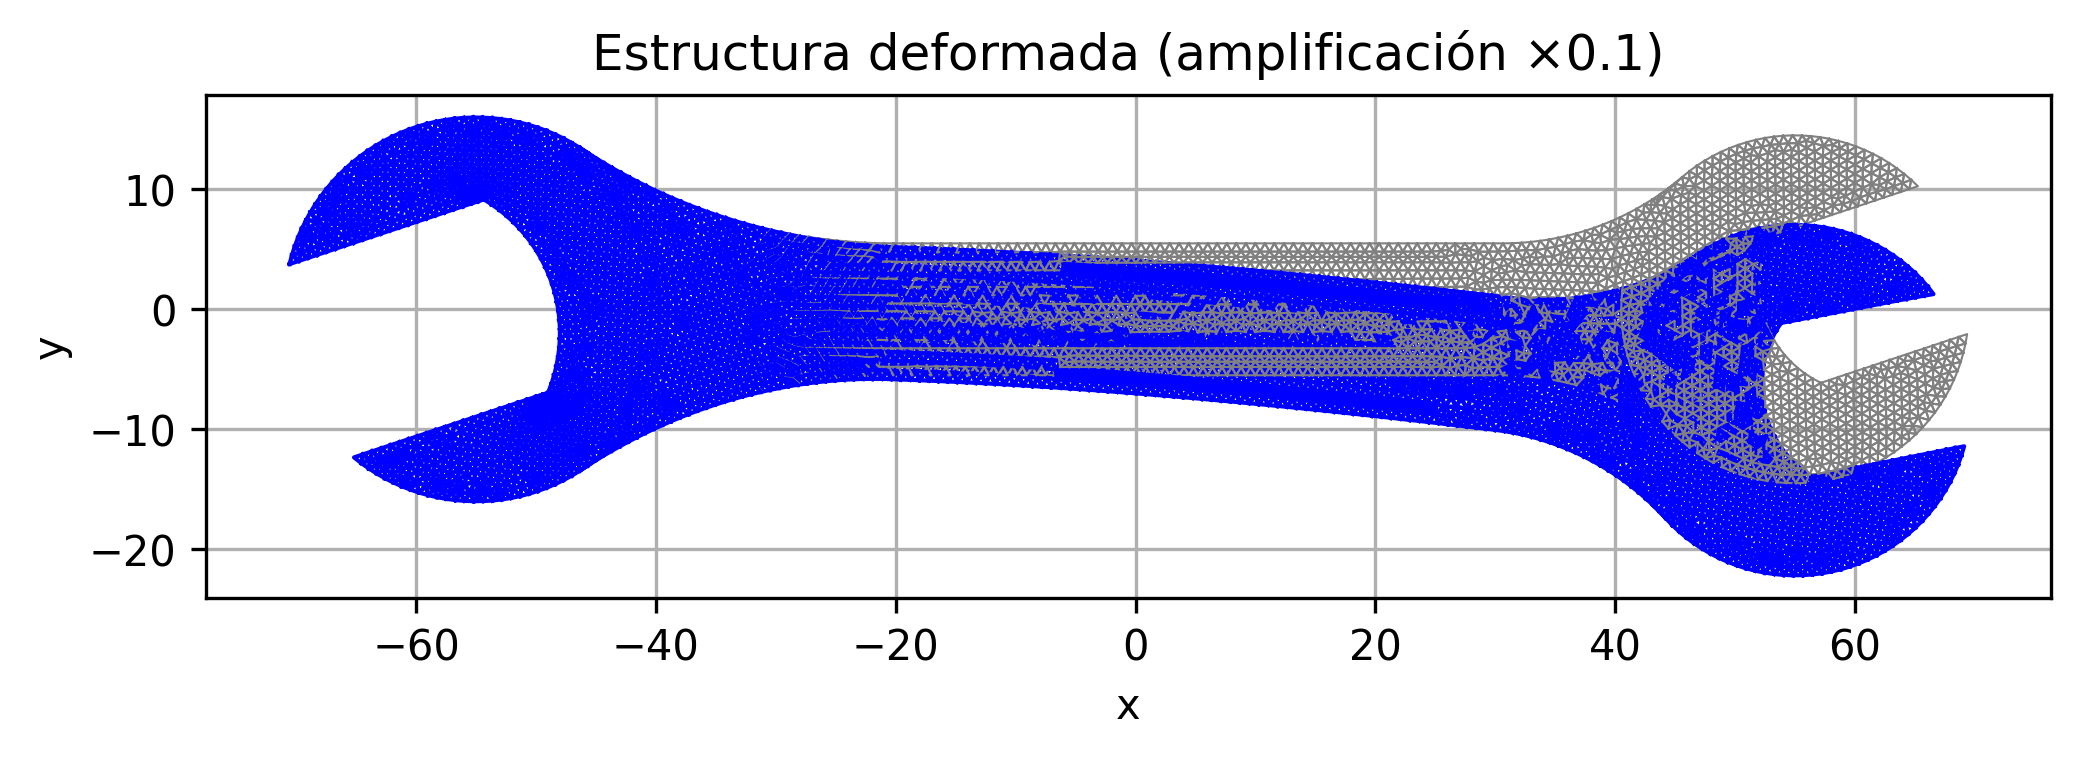
\includegraphics[width=0.8\textwidth]{GRAFICOS/Case a_deformada.png}
    \caption{Deformed wrench with point load}
    \label{fig:xdi}
\end{figure}

In the following tables, the stress and strain components are shown.

\begin{table}[H]
    \centering
    \caption{Stress (Pa) and strain components}
    \begin{tabular}{|c|c|c|c|c|c|}
    \hline
    $\sigma_{xx}$ & $\sigma_{yy}$ & $\tau_{xy}$ & $\epsilon_{xx}$ & $\epsilon_{yy}$ & $\gamma_{xy}$ \\
    \hline
    450 & 72 & -120 & 0.12 & 0.045 & -0.096 \\
    \hline
    \end{tabular}
    \label{tab:tabla1}
\end{table}
    
\begin{table}[H]
    \centering
    \caption{Principal Stresses (Pa) and strain components}
    \begin{tabular}{|c|c|c|c|}
    \hline
    $\sigma_{1}$ & $\sigma_{2}$ & $\epsilon_{1}$ & $\epsilon_{2}$ \\
    \hline
    450 & -450 & 0.128 & -0.128 \\
    \hline
    \end{tabular}
    \label{tab:tabla2}
\end{table}


It is noticeable that, compared to the previous case, the principal strains are significally higher. This is due to the fact that considering the type of material and its mechanical properties, the force magnitude and single point of application increases the stress concentration throughout the wrench. This is also reflected in the Von Misses stress, which reaches a maximum value of $\sigma_{VM} = 450 Pa$.

\begin{figure}[H]
    \centering
    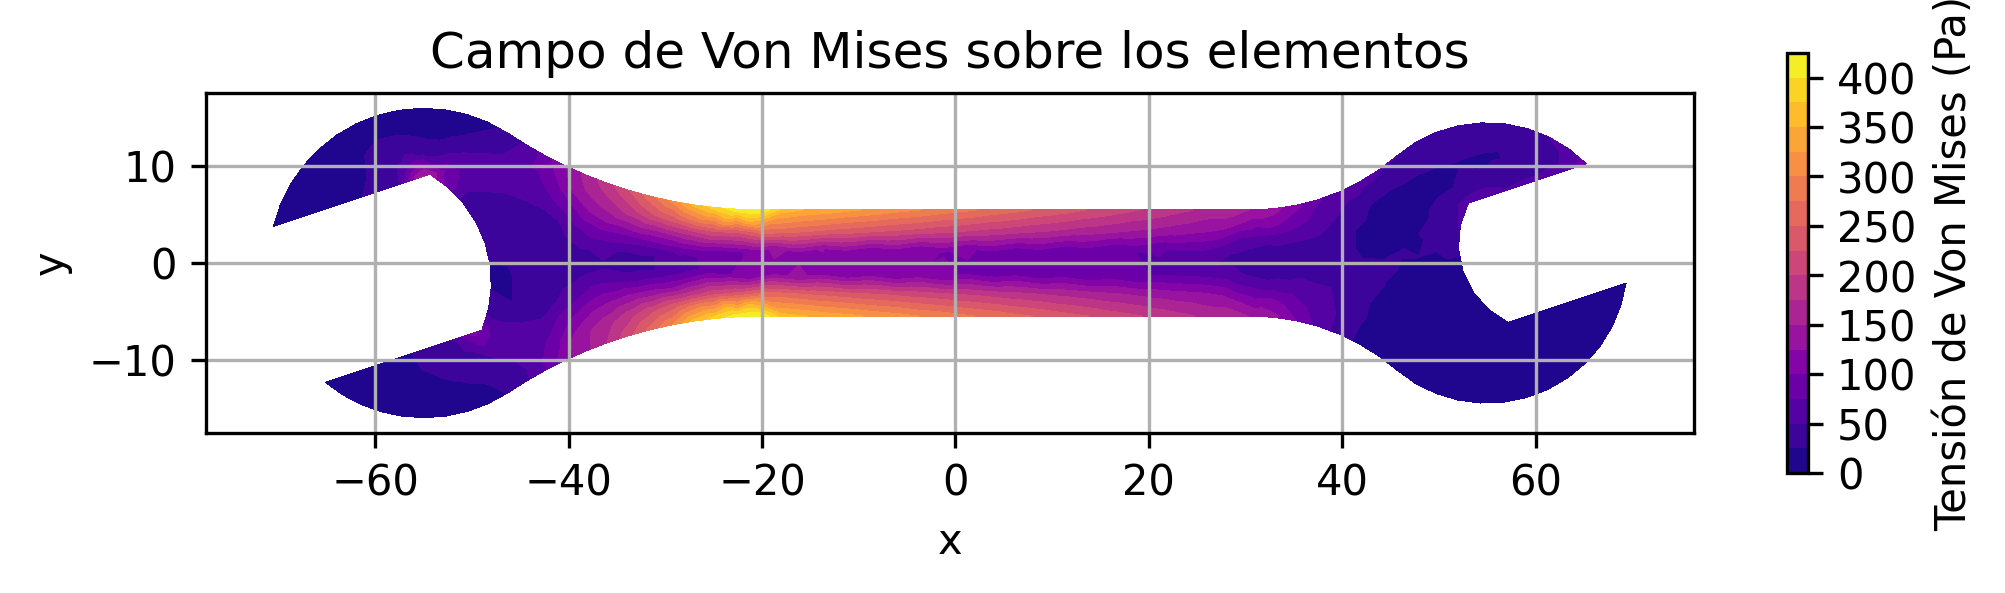
\includegraphics[width=0.8\textwidth]{GRAFICOS/Case a_von_mises.png}
    \caption{Von Misses stress distribution for the point load}
    \label{fig:principal}
\end{figure}

\subsection{Case 3: Self-weight added to the distributed load}

Now, a similar case to the first one was analyzed, but this time the self-weight was added as a body force ($m_{wrench} = 8 gr$). The results are shown below.

\begin{figure}[H]
    \centering
    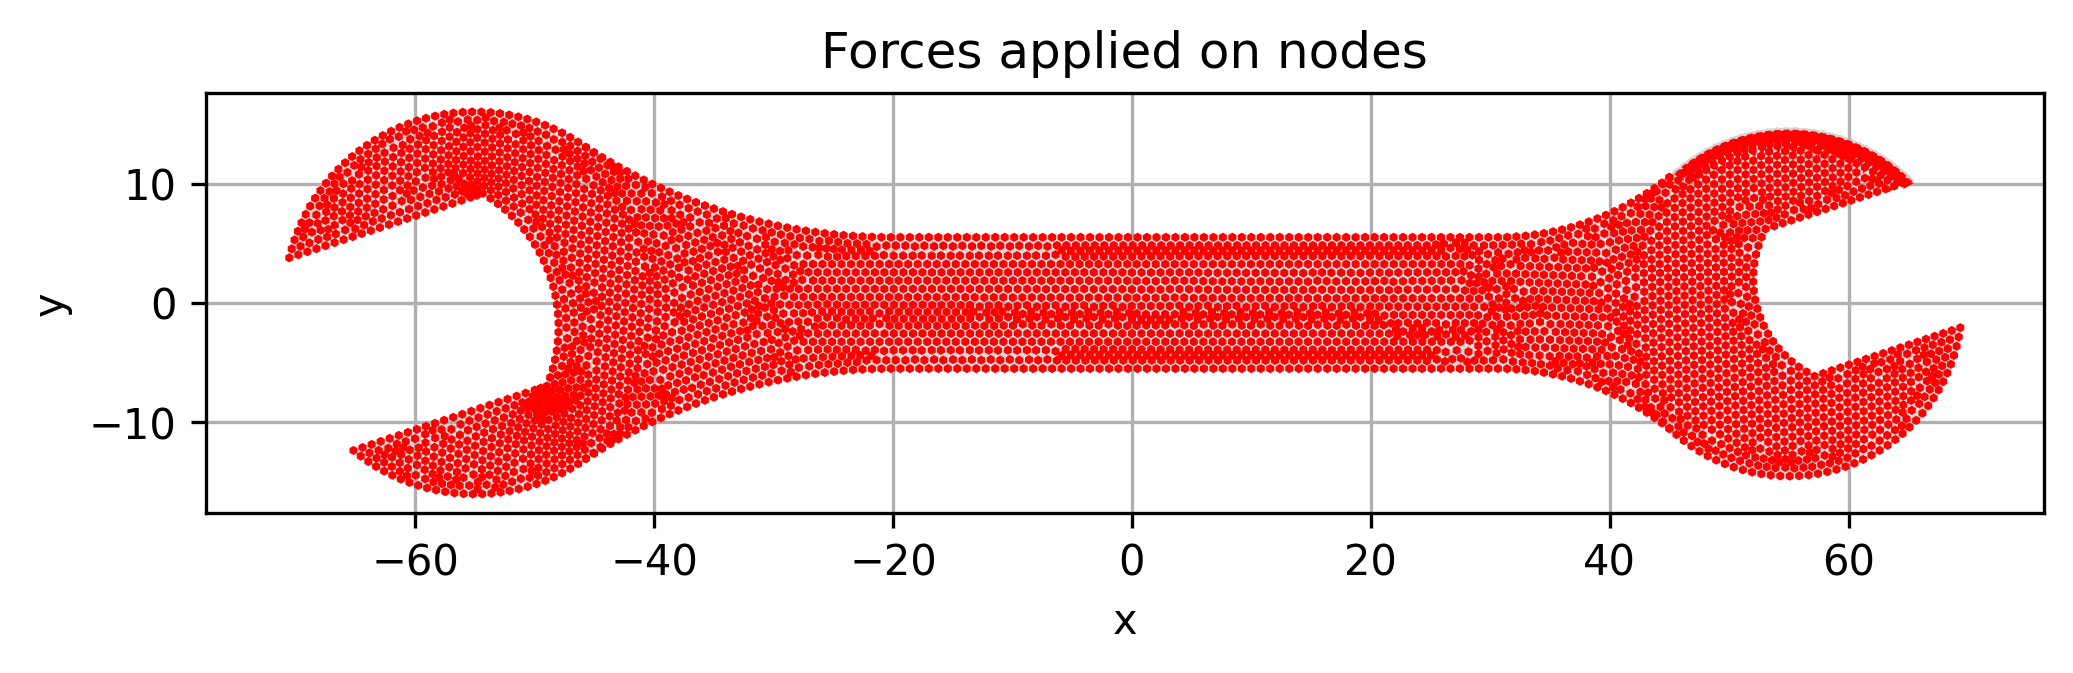
\includegraphics[width=0.8\textwidth]{GRAFICOS/Case c_fuerzas.png}
    \caption{Applied self-weight forces acting on each CST element's centroid.}
    \label{fig:xdiwi}
\end{figure}

We can observe in Figure \ref{fig:xdiwi} that the self-weight vector acts across the entire body of the wrench, specifically at the mass centroid of each CST element.  
The deformed state of the structure is shown in Figure \ref{fig:xdiwi2}.

\begin{figure}[H]
    \centering
    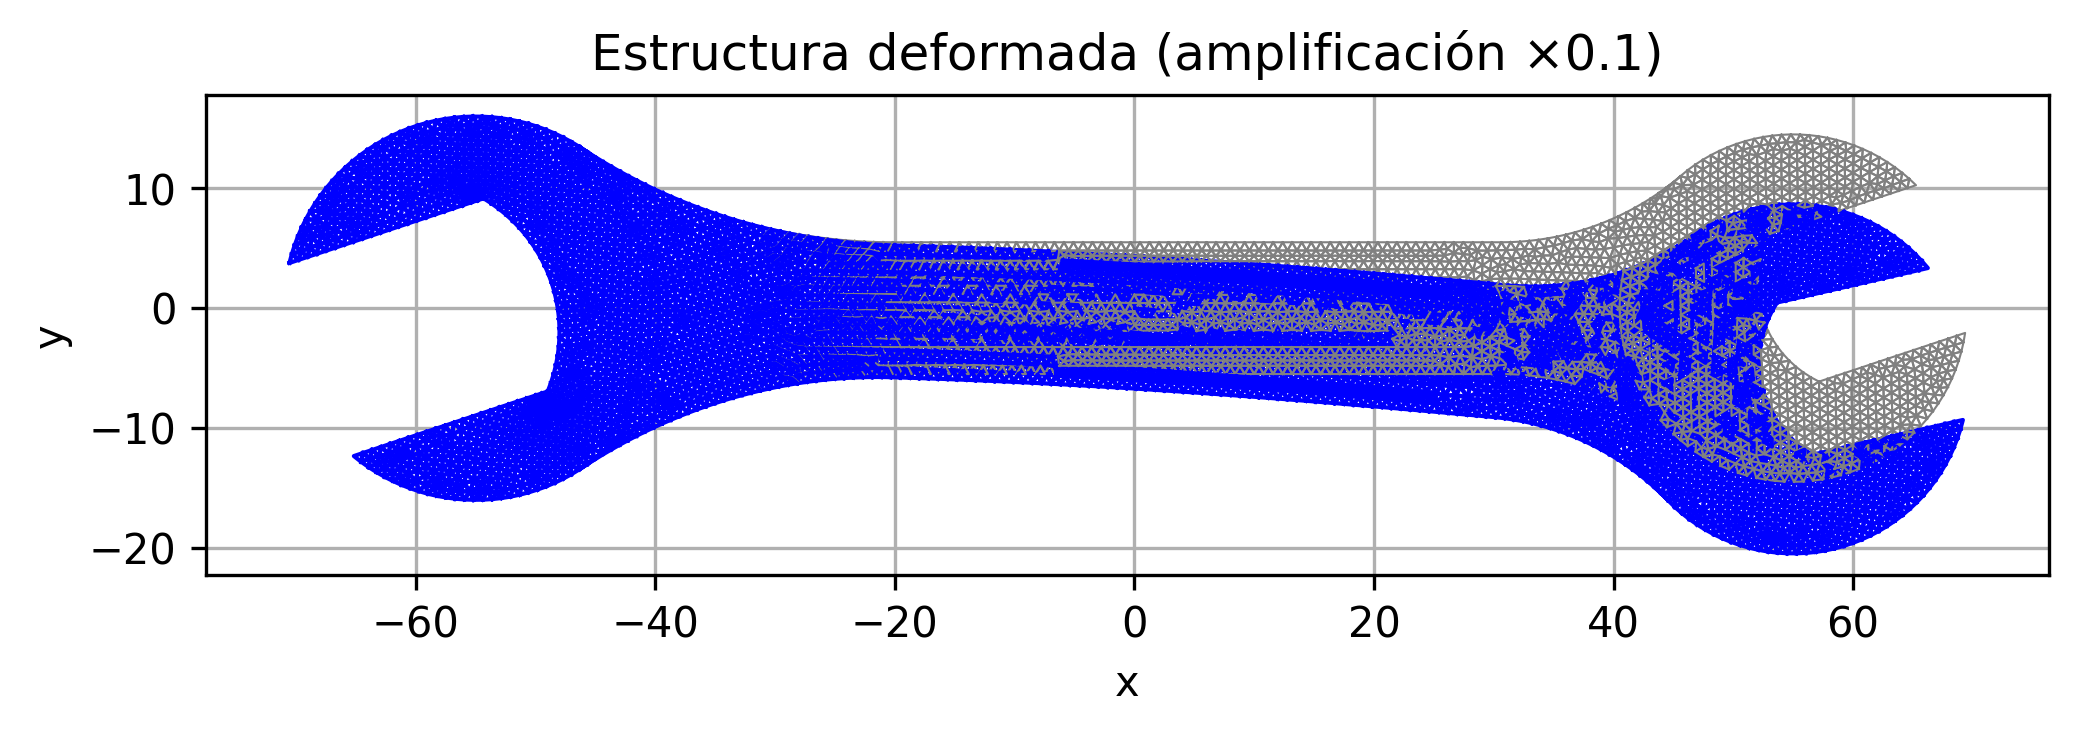
\includegraphics[width=0.8\textwidth]{GRAFICOS/Case c_deformada.png}
    \caption{Deformed configuration of the wrench under self-weight loading.}
    \label{fig:xdiwi2}
\end{figure}


\begin{table}[H]
    \centering
    \caption{Stress (Pa) and strain components}
    \begin{tabular}{|c|c|c|c|c|c|}
    \hline
    $\sigma_{xx}$ & $\sigma_{yy}$ & $\tau_{xy}$ & $\epsilon_{xx}$ & $\epsilon_{yy}$ & $\gamma_{xy}$ \\
    \hline
    360 & 60 & -60 & 0.09 & 0.036 & -0.05 \\
    \hline
    \end{tabular}
    \label{tab:tabla1}
\end{table}
    
\begin{table}[H]
    \centering
    \caption{Principal Stresses (Pa) and strain components}
    \begin{tabular}{|c|c|c|c|}
    \hline
    $\sigma_{1}$ & $\sigma_{2}$ & $\epsilon_{1}$ & $\epsilon_{2}$ \\
    \hline
    360 & -360 & 0.108 & -0.108 \\
    \hline
    \end{tabular}
    \label{tab:tabla2}
\end{table}

Comparing this scenario with the one presented in Case 1, the results are the same. This is because the self-weight of the wrench is negligible compared to the distributed load of $30 kgf$. Therefore, the internal stresses and strains are not affectedd by it.

\subsection{Case 4: Only self-weight applied as a body force}

The decision to analyze this singular case was made in order to observe and compere how this body force condition affected the wrench. This way, we can observe that, due to the conditions of restrcited nodes in one end, the wrench still deforms, but in a much smaller magnitude.

\begin{figure}[H]
    \centering
    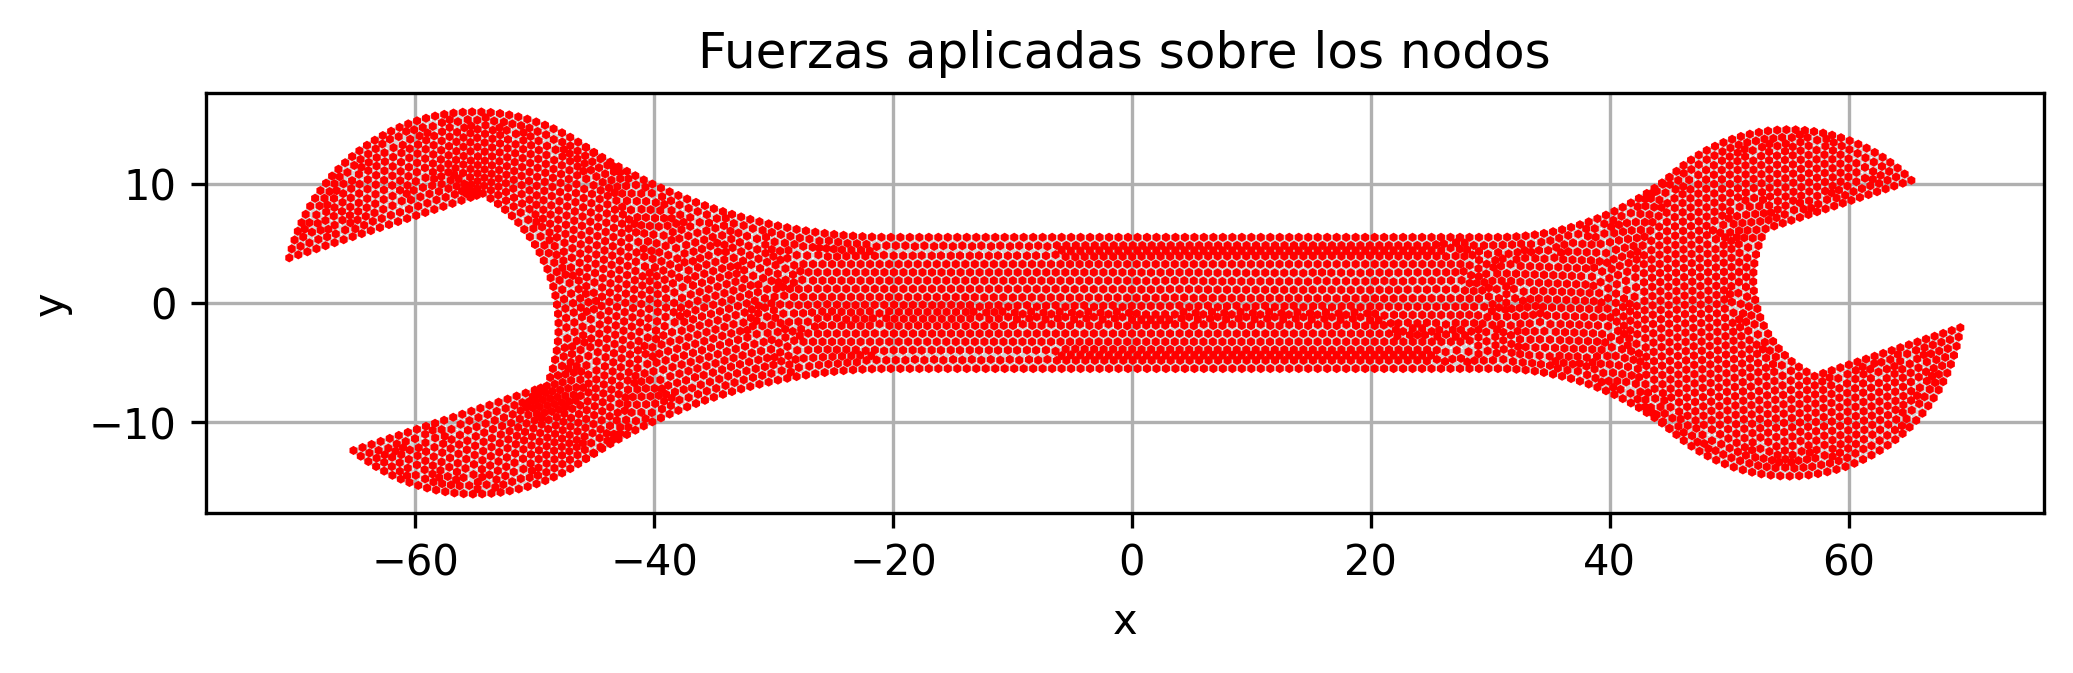
\includegraphics[width=0.8\textwidth]{GRAFICOS/Case d_fuerzas.png}
    \caption{Self-weight applied as a body force}
    \label{fig:bf}
\end{figure}

\begin{figure}[H]
    \centering
    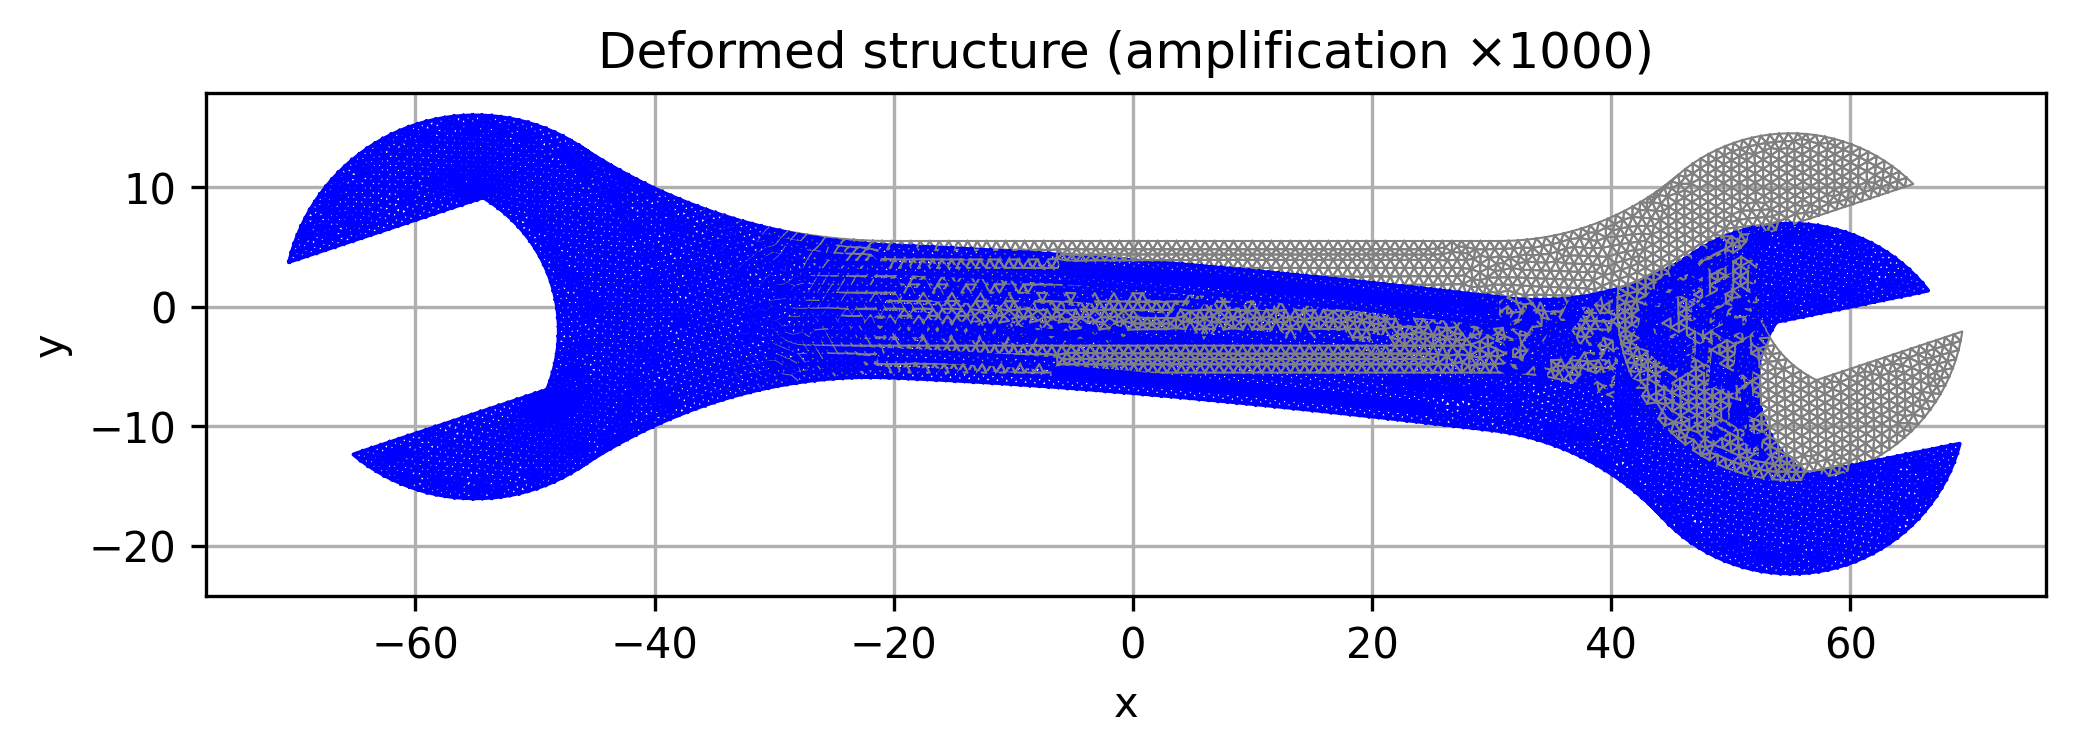
\includegraphics[width=0.8\textwidth]{GRAFICOS/Case d_deformada.png}
    \caption{Deformed wrench with self-weight}
    \label{fig:bf1}
\end{figure}

Notice the amplification factor of the deformed state, which is $10^3$. Which is a clear indication of the small magnitude of the displacements compared to the previous 3 cases. The stress and strain components are shown below.

\begin{table}[H]
    \centering
    \caption{Stress (Pa) and strain components}
    \begin{tabular}{|c|c|c|c|c|c|}
    \hline
    $\sigma_{xx}$ & $\sigma_{yy}$ & $\tau_{xy}$ & $\epsilon_{xx}$ & $\epsilon_{yy}$ & $\gamma_{xy}$ \\
    \hline
    0.045 & 0.012 & -0.0096 & $1.35\times10^{-5}$ & $4.5\times10^{-6}$ & $6.4\times10^{-6}$ \\
    \hline
    \end{tabular}
    \label{tab:tabla1}
\end{table}
    
\begin{table}[H]
    \centering
    \caption{Principal Stresses (Pa) and strain components}
    \begin{tabular}{|c|c|c|c|}
    \hline
    $\sigma_{1}$ & $\sigma_{2}$ & $\epsilon_{1}$ & $\epsilon_{2}$ \\
    \hline
    0.048 & -0.0525 & $1.44\times10^{-5}$ & $-1.44\times10^{-5}$ \\
    \hline
    \end{tabular}
    \label{tab:tabla2}
\end{table}

Observing the plot of the Von Mises stresses, we can see that the maximum value is $\sigma_{VM} = 0.0525\ \text{Pa}$.  
This clearly indicates the low impact of the self-weight on the wrench structure.

\begin{figure}[H]
    \centering
    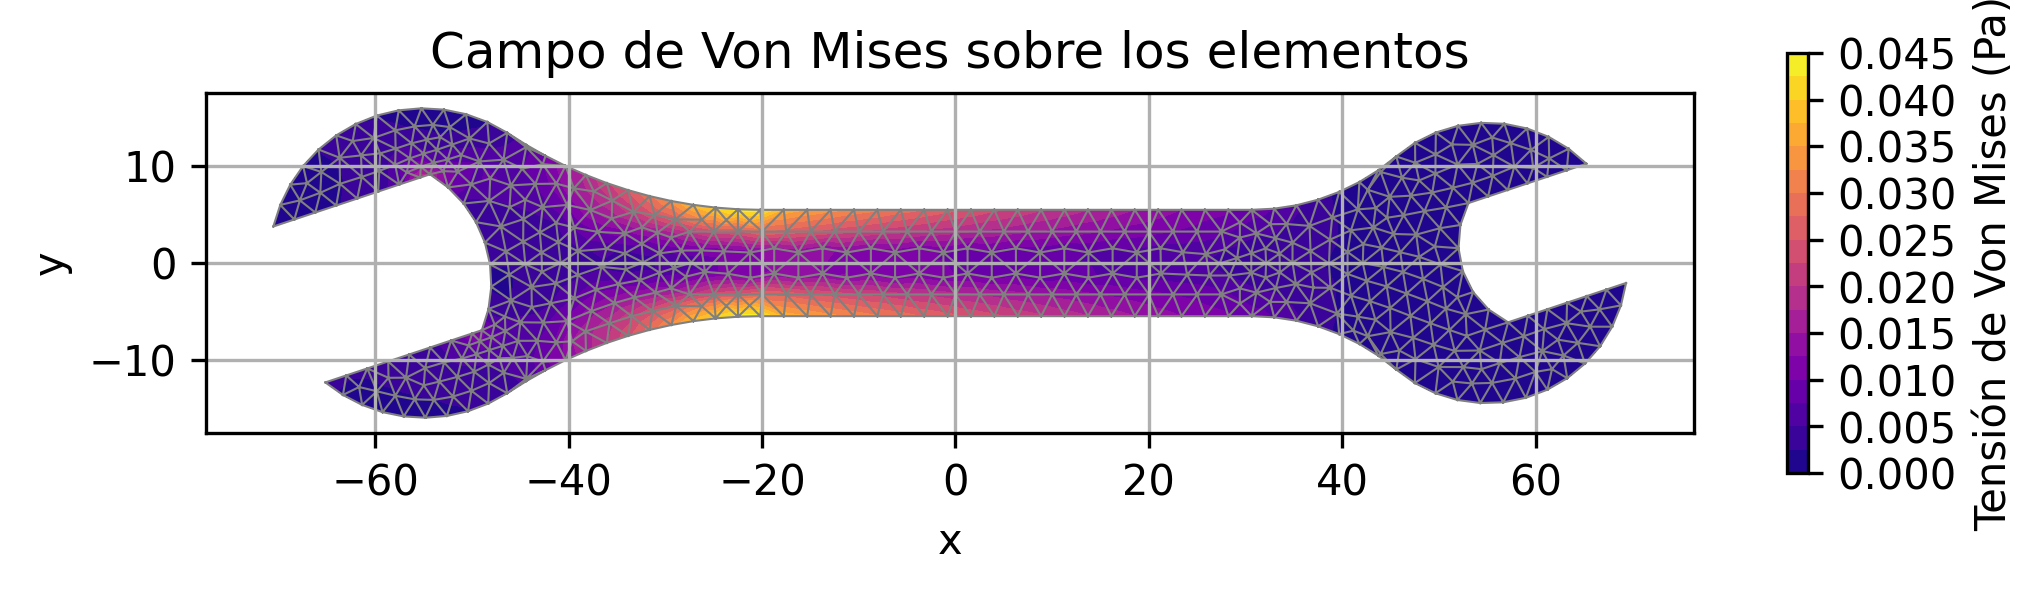
\includegraphics[width=0.8\textwidth]{GRAFICOS/Case d_von_mises.png}
    \caption{Von Mises stress distribution under self-weight loading.}
    \label{fig:principal}
\end{figure}


Finally, the simulation shows the clear mechanical behavior of the PLA wrench under different loading conditions. Where the CST model was able to capture accuratly and with precision the internal stresses and strains of the element. The results were coherent with the physical behavior of it, and the Von Misses stress was able to capture the stress concentration in the areas of interest. The results were also consistent with the expected behavior of a wrench under different loading conditions.





\section{Preguntas}

\subsection{How do you know convergence in mesh size has been achieved?}

Mesh size convergence is achieved when the solution of the problem does not change significantly with a further refinement of the mesh. This can be checked by comparing the results of the displacements, Von Mises stresses and principal stresses compared to other mesh sizes. In this case, convergence was assessed by plotting the maximum Von misses Stress with the characteristic lenght, and observing the time of processing in each case. The result shows that at an $L_c$ of 0.8, the mesh was already converging.

\begin{figure}[H]
\centering
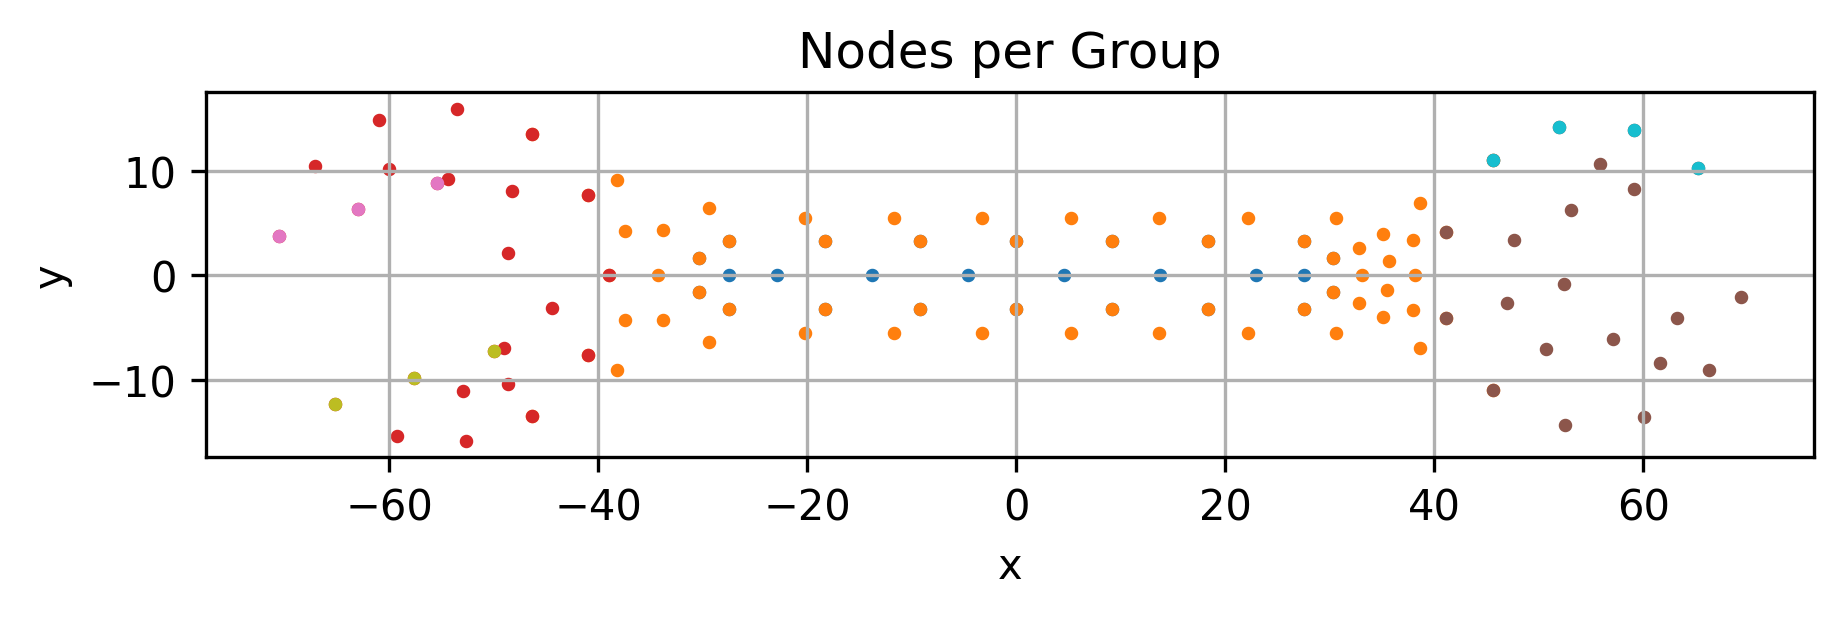
\includegraphics[width=0.5\textwidth]{GRAFICOS/Initial_nodes_por_grupo.png}
\caption{Caption}
\label{fig:wrench}
\end{figure}
  
\begin{figure}[H]
\centering
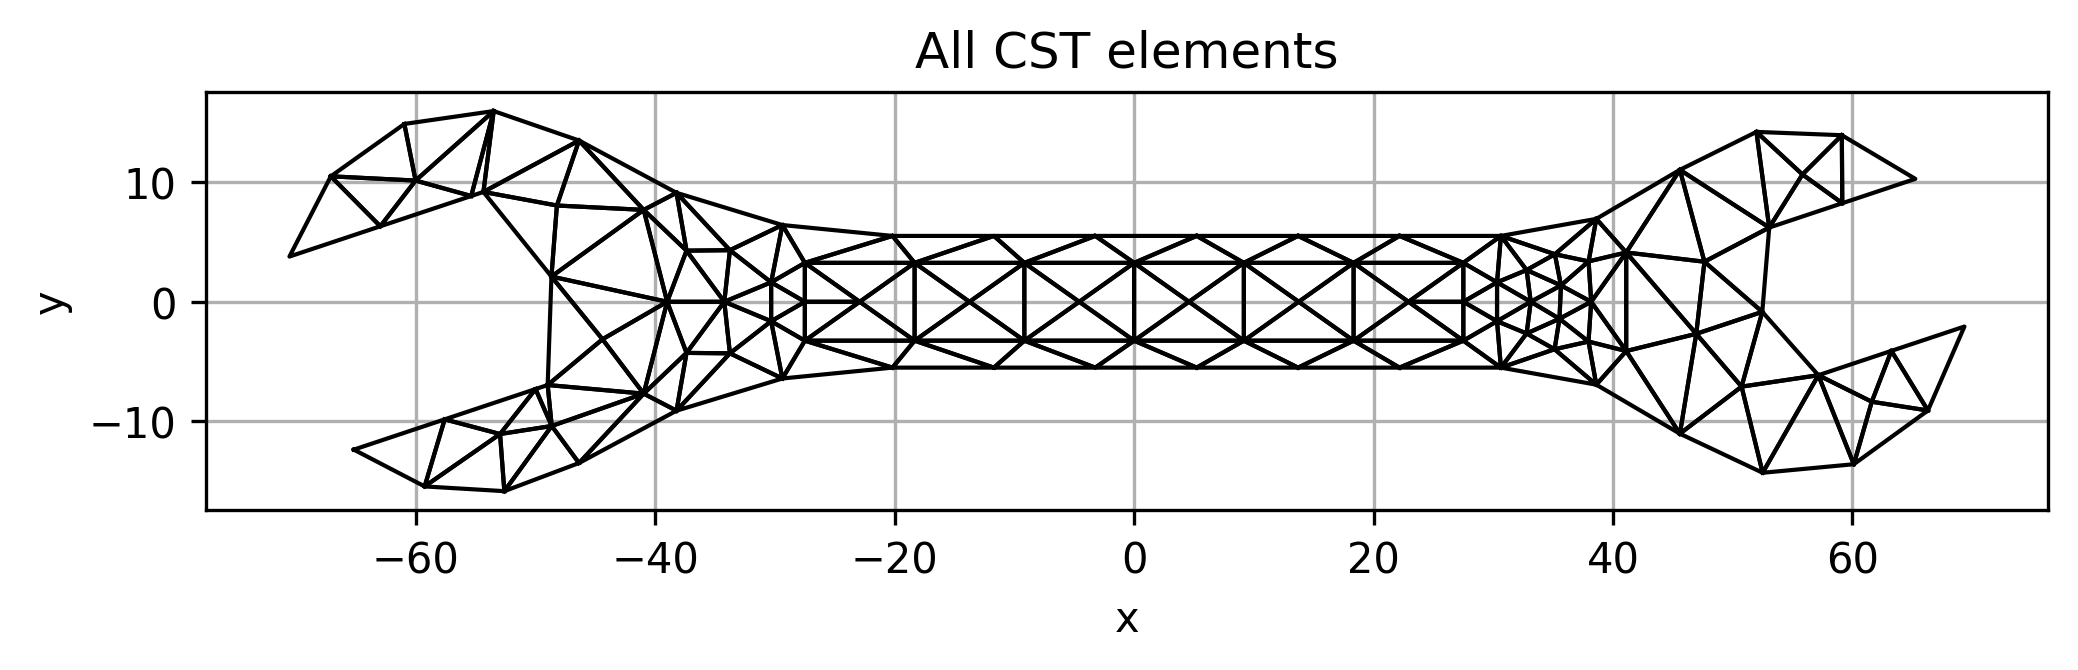
\includegraphics[width=0.5\textwidth]{GRAFICOS/Initial_elementos.png}
\caption{Caption}
\label{fig:deformed_shape}
\end{figure}
  
Then, a code was programmed to plot the convergence of the mesh depending on the time of ejecution.
  
\begin{figure}[H]
\centering
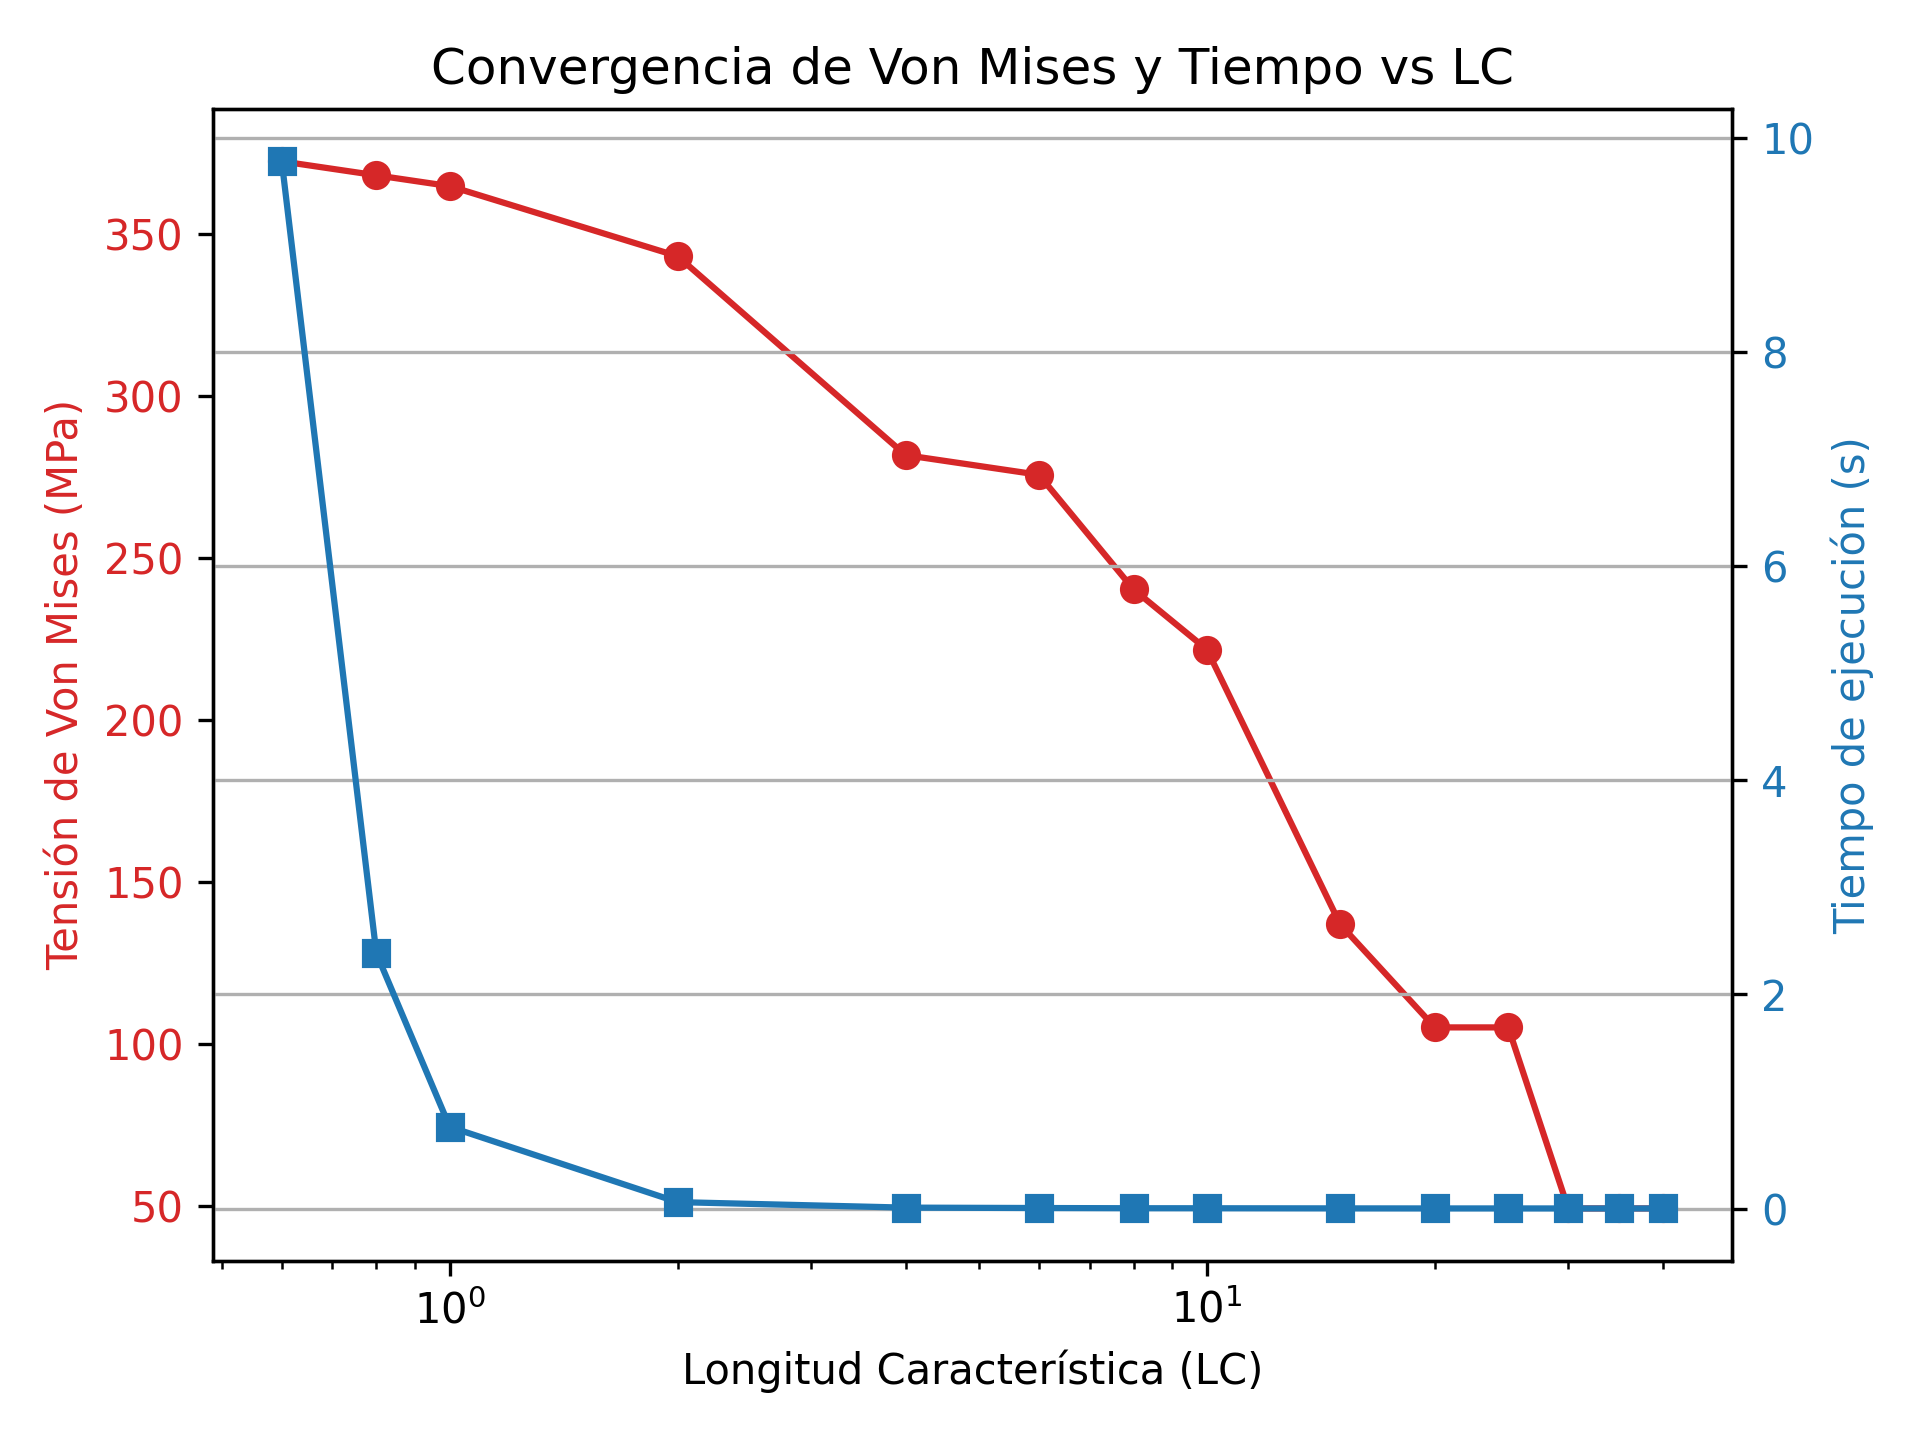
\includegraphics[width=0.6\textwidth]{GRAFICOS/convergencia.png}
\caption{Caption}
\label{fig:wrench}
\end{figure}

The result was an $L_c = 0.8$, balancing the time of computation and the precision of the model.

Therefore, the final model is plotted as follows:
  
\begin{figure}[H]
\centering
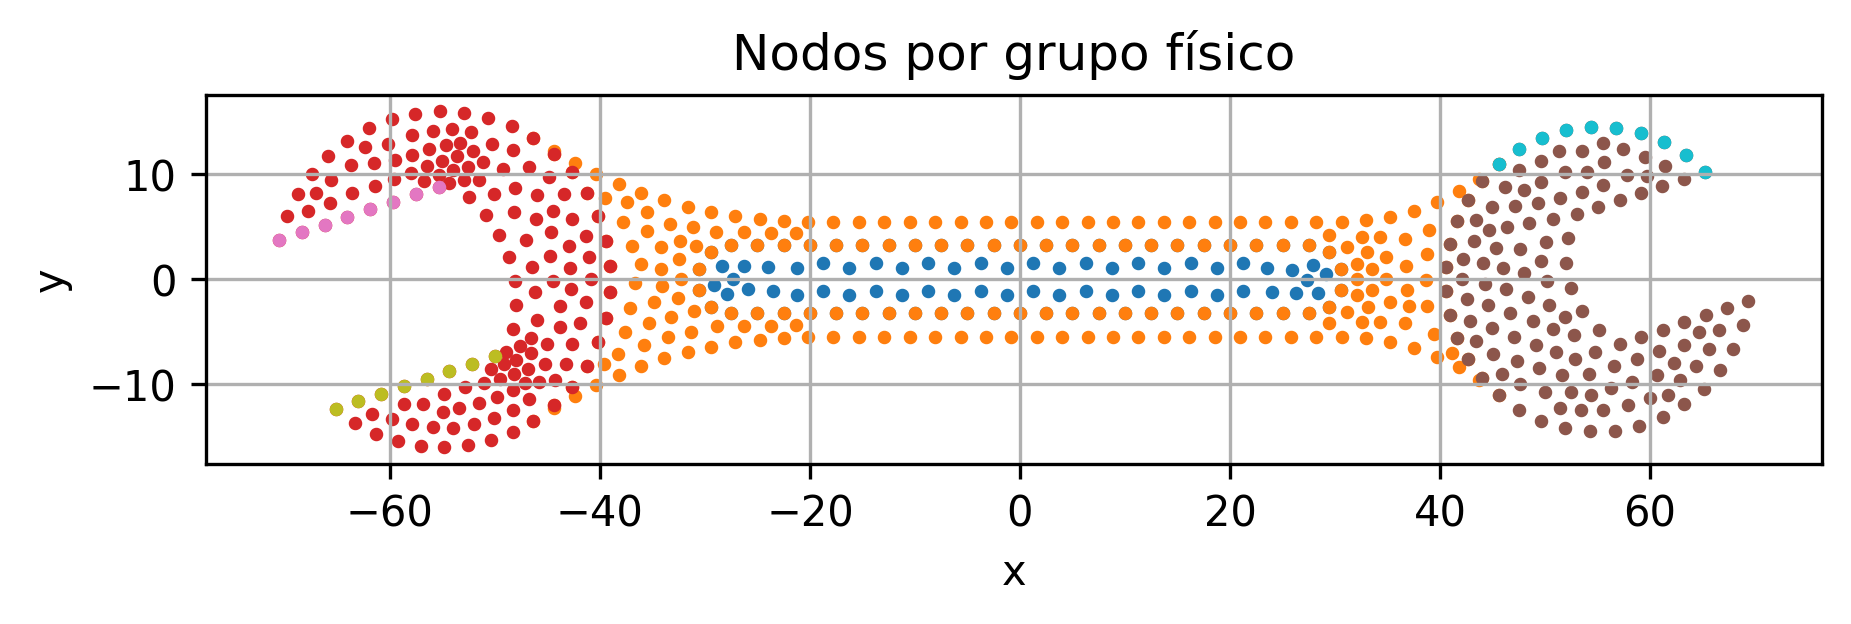
\includegraphics[width=0.5\textwidth]{GRAFICOS/Case a_nodes_por_grupo.png}
\caption{Caption}
\label{fig:wrench}
\end{figure}
  
\begin{figure}[H]
\centering
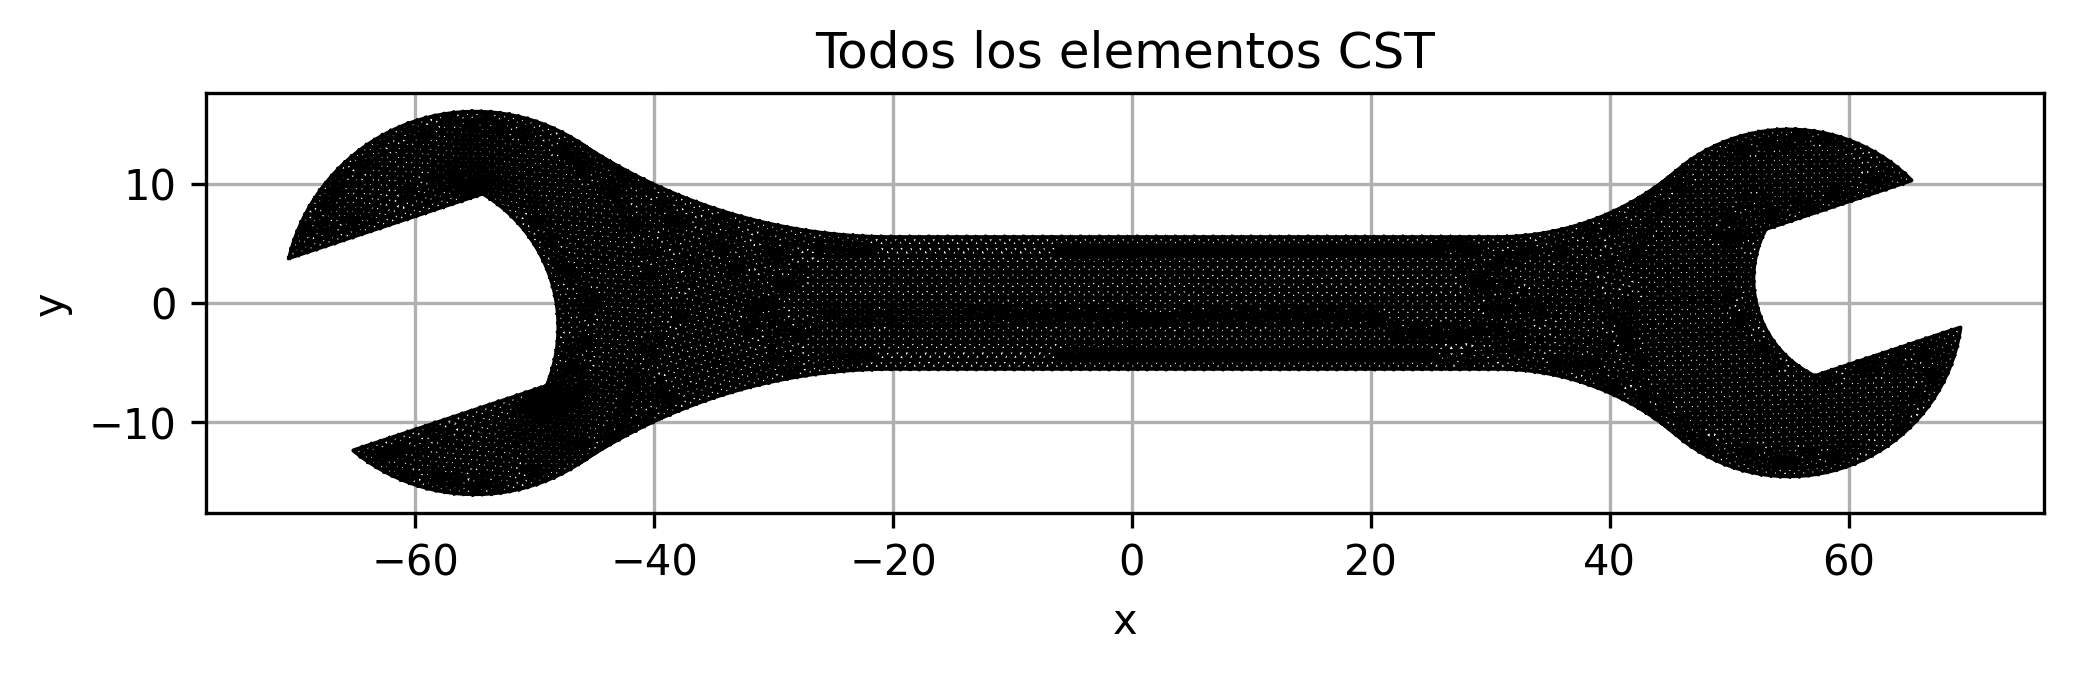
\includegraphics[width=0.5\textwidth]{GRAFICOS/Case a_elementos.png}
\caption{Caption}
\label{fig:deformed_shape}
\end{figure}

\subsection{How do the stress/strain fields look like before and after smoothing?}

Before smoothing, the stress and strain fields shows abrubt jumps between adjacent elements, producing a non-physical behaviour and dicontinuous fields. It is expected due to the implementation of CST elements, which have a constant stress and strain state. After applying post-processing smoothing, the fields becmoe continuous, whit better transitions across the domain, making it physically accurate.

\subsection{What differences do you observe when applying the load as a distributed load versus a point load?}

As a distributed load results in smoother and more realistic stress fiels, as the force is spread over an area, avoiding axcessive stress concentrations. 
On the other hand, a point load produces localized hight-stress peaks near the application point, leading to unrealistic stress values, unless the mesh is highly refined.

\subsection{Is it necessary to consider self-weight for an accurate analysis of the tool?}

In this case, it is not necessary to consider it, because the external forces applied are significantly grater than de self-weight of the PLA material. 
However, numercial comparisons showed that including self-weight, slightly increases the overall stress and displacement values, especially un ling or thin sections.

\subsection{Research or provide a reasonable stress-based failure criteria for PLA. For this loading condition, and based on
your failure criteria ¿where do you expect the wrench to fail?}

According to \citet{farah2016}, PLA (Polylactic Acid) exhibits a tensile strength near 50 MPa, depending on molecular weight, crystallinity, and processing method. Additionally, the usual Young's module is about 3.5 GPa, and the material has a relatively low elongation at break (about $4\text{-}7\%$), confirming its brittle nature.

Therefore, a reasonable stress-based failure criteria for PLA under mechanical loading is the Von Mises yield criterion, assuming brittle fracture at an equivalent stress level of around 50 MPa. Given PLA's limited ductility and tendency to fail without significant plastic deformation, reaching the ultimate tensile strength would iniciate cracking or brittle rupture.

As a result, based on the FEM simulations and stress distribution results, the highest Von Mises stresses concentrated at the junction between the wrench handle and the wrench head would be an expected failure location, in other words, near sharp geometrical transitions or areas under bending moments.












\section{Anexos}

\subsection{Case A}

\begin{figure}[H]
    \centering
    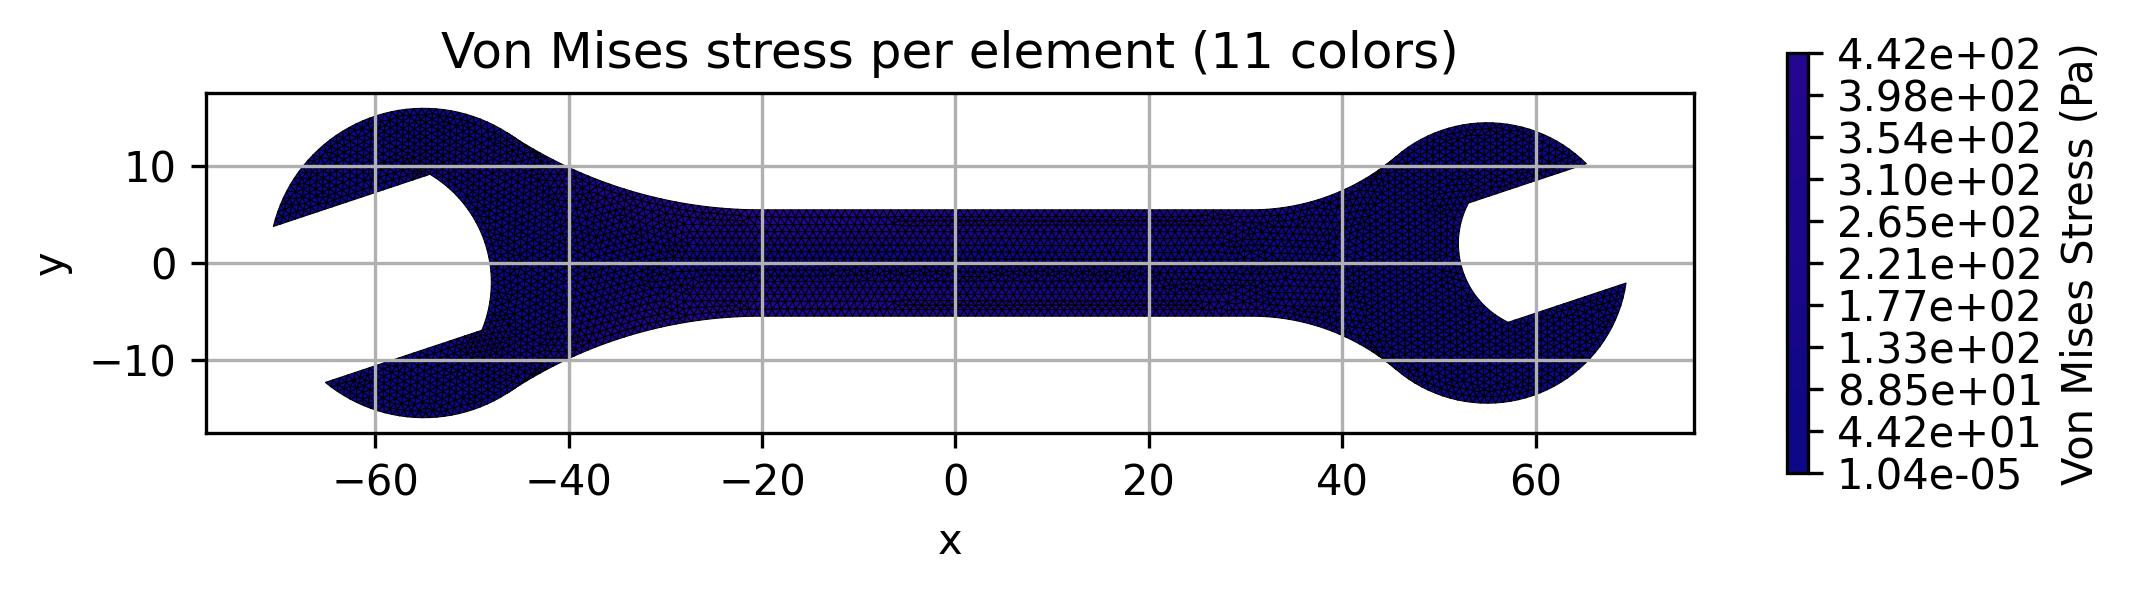
\includegraphics[width=0.8\textwidth]{GRAFICOS/Case a_von_mises_per_element_11_colors.png}
    \caption{Caption}
    \label{fig:strain}
  \end{figure}

  \begin{figure}[H]
    \centering
    \begin{subfigure}[t]{0.49\textwidth}
      \centering
      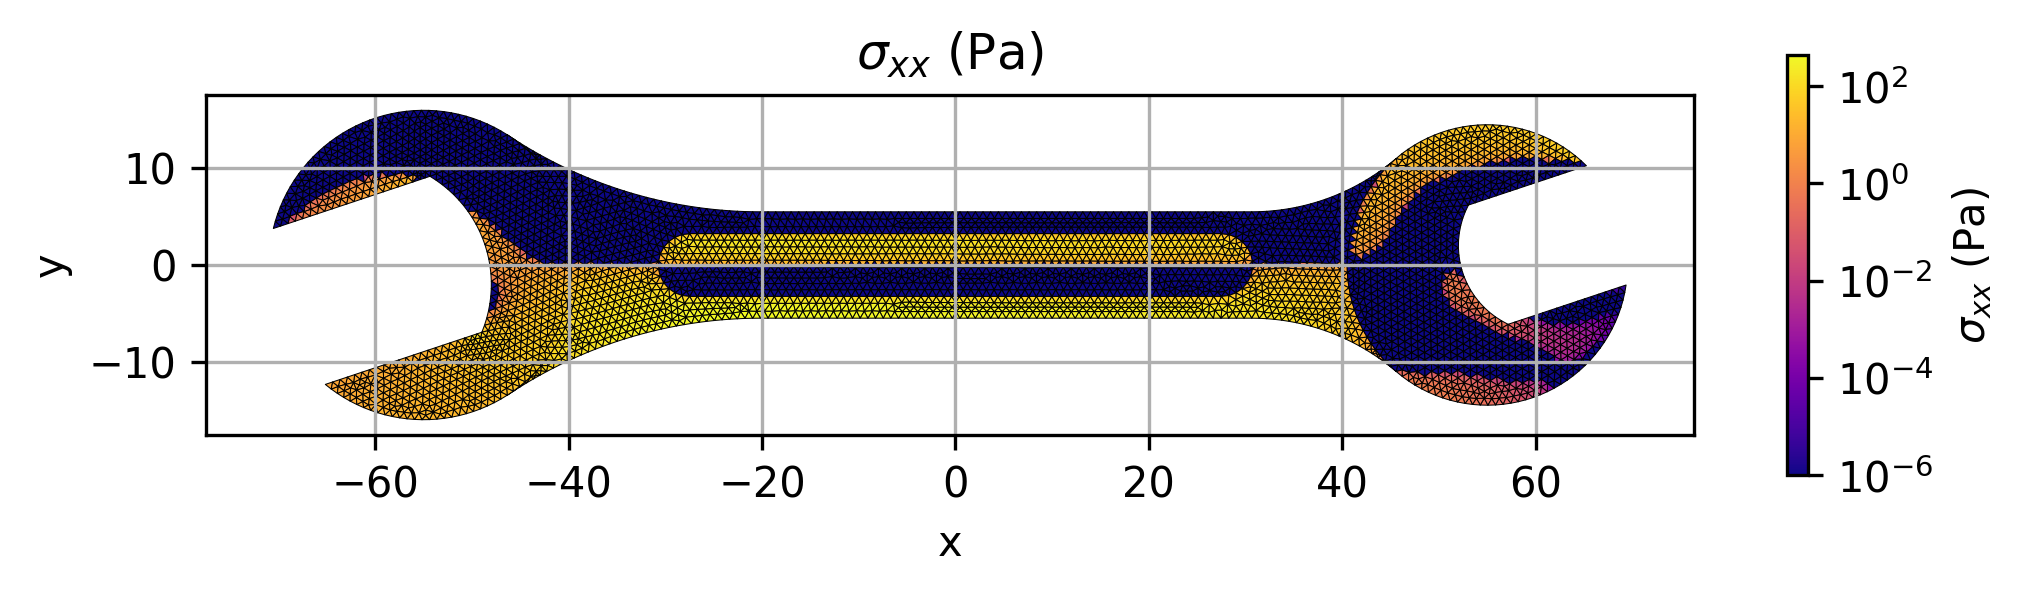
\includegraphics[width=\textwidth]{GRAFICOS/Case a - sigma_xx_per_element.png}
      \caption{Caption}
      \label{fig:deformada_reacciones}
    \end{subfigure}
    \hfill
    \begin{subfigure}[t]{0.49\textwidth}
      \centering
      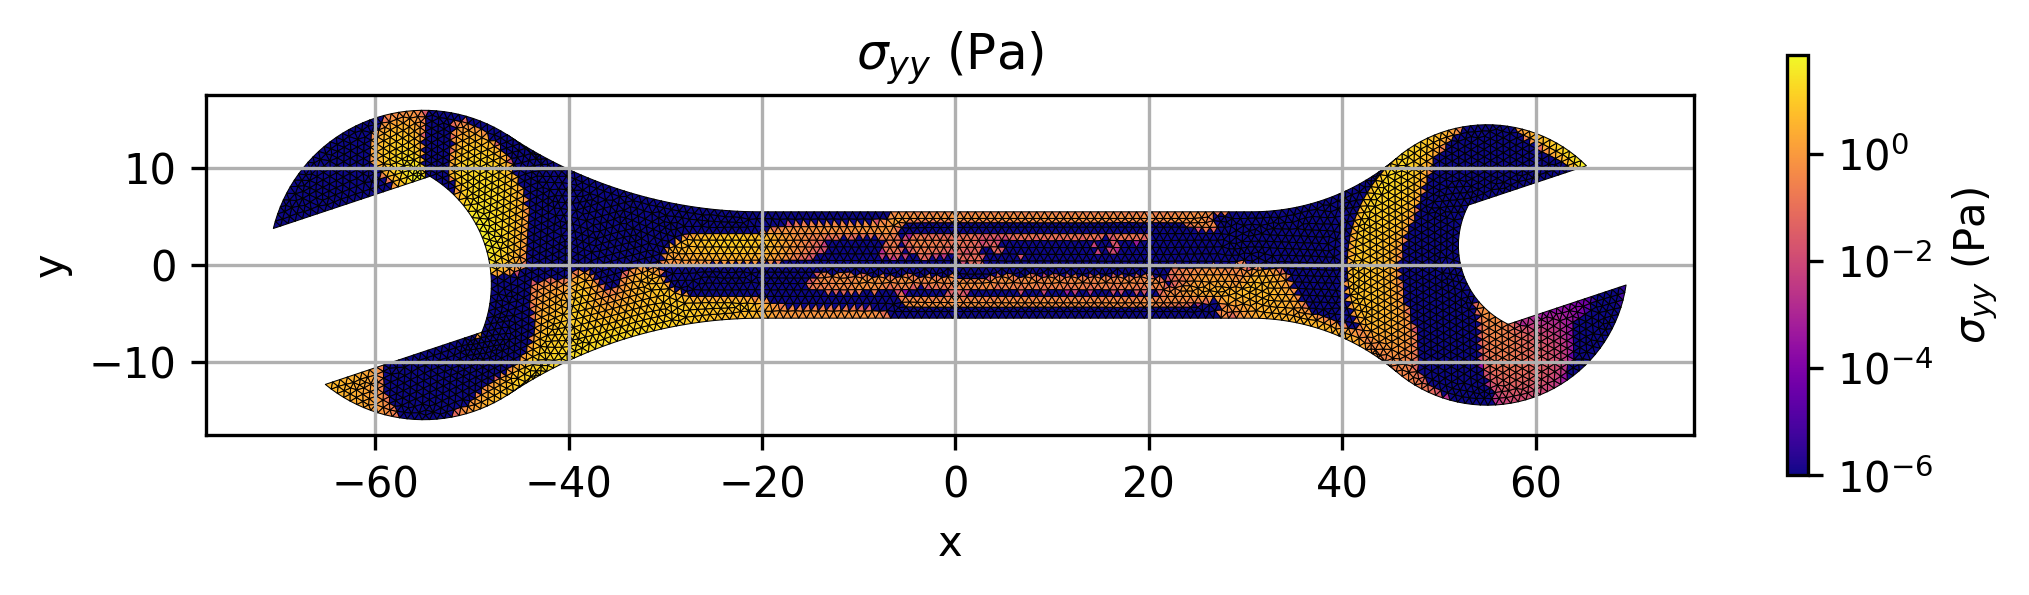
\includegraphics[width=\textwidth]{GRAFICOS/Case a - sigma_yy_per_element.png}
      \caption{Caption}
      \label{fig:von_mises}
    \end{subfigure}
    \caption{Caption}
    \label{fig:analisis_estructural}
  \end{figure}

  \begin{figure}[H]
    \centering
    \begin{subfigure}[t]{0.49\textwidth}
      \centering
      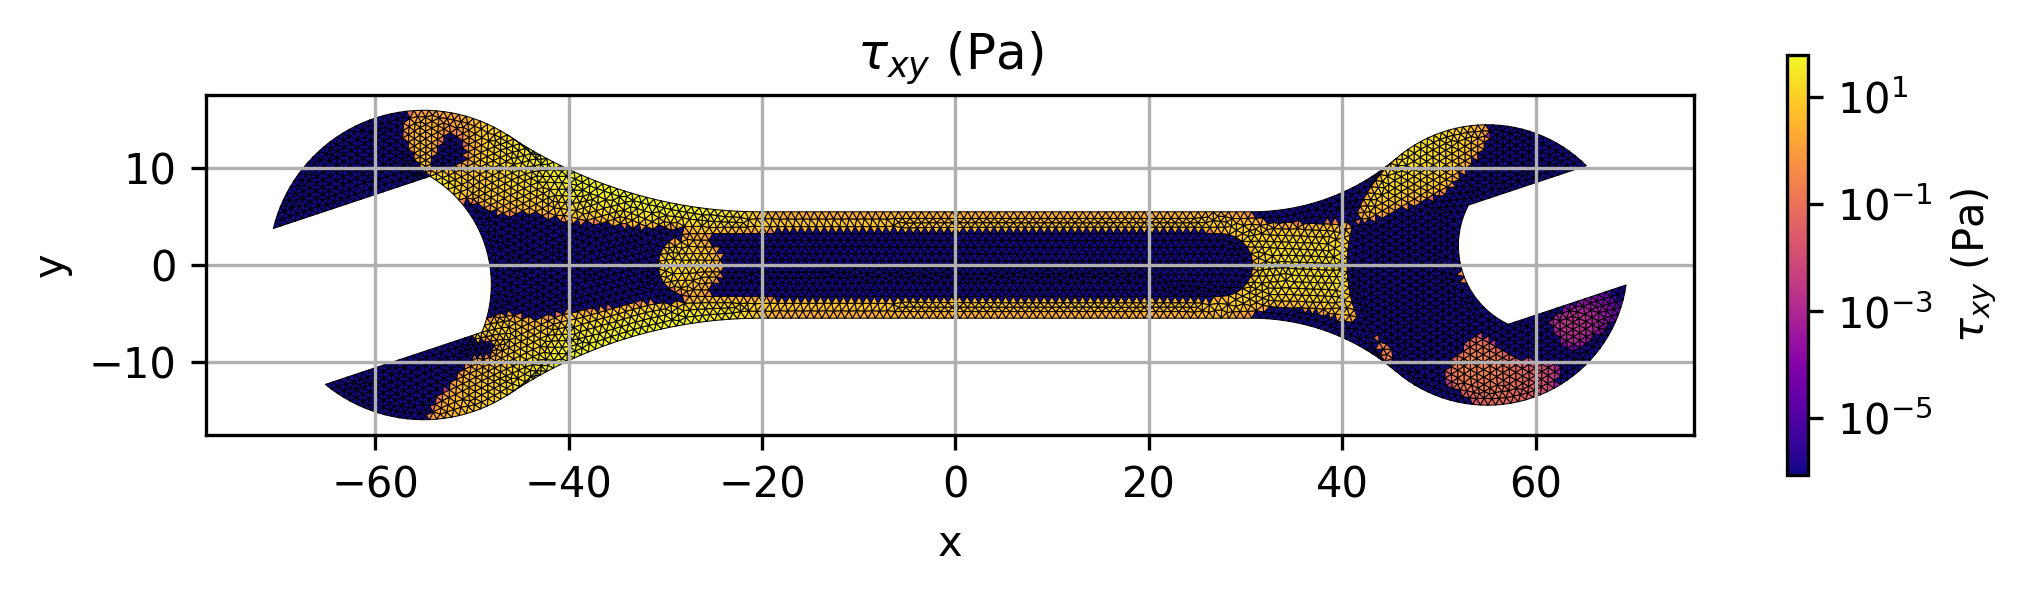
\includegraphics[width=\textwidth]{GRAFICOS/Case a - tau_xy_per_element.png}
      \caption{Caption}
      \label{fig:deformada_reacciones}
    \end{subfigure}
    \hfill
    \begin{subfigure}[t]{0.49\textwidth}
      \centering
      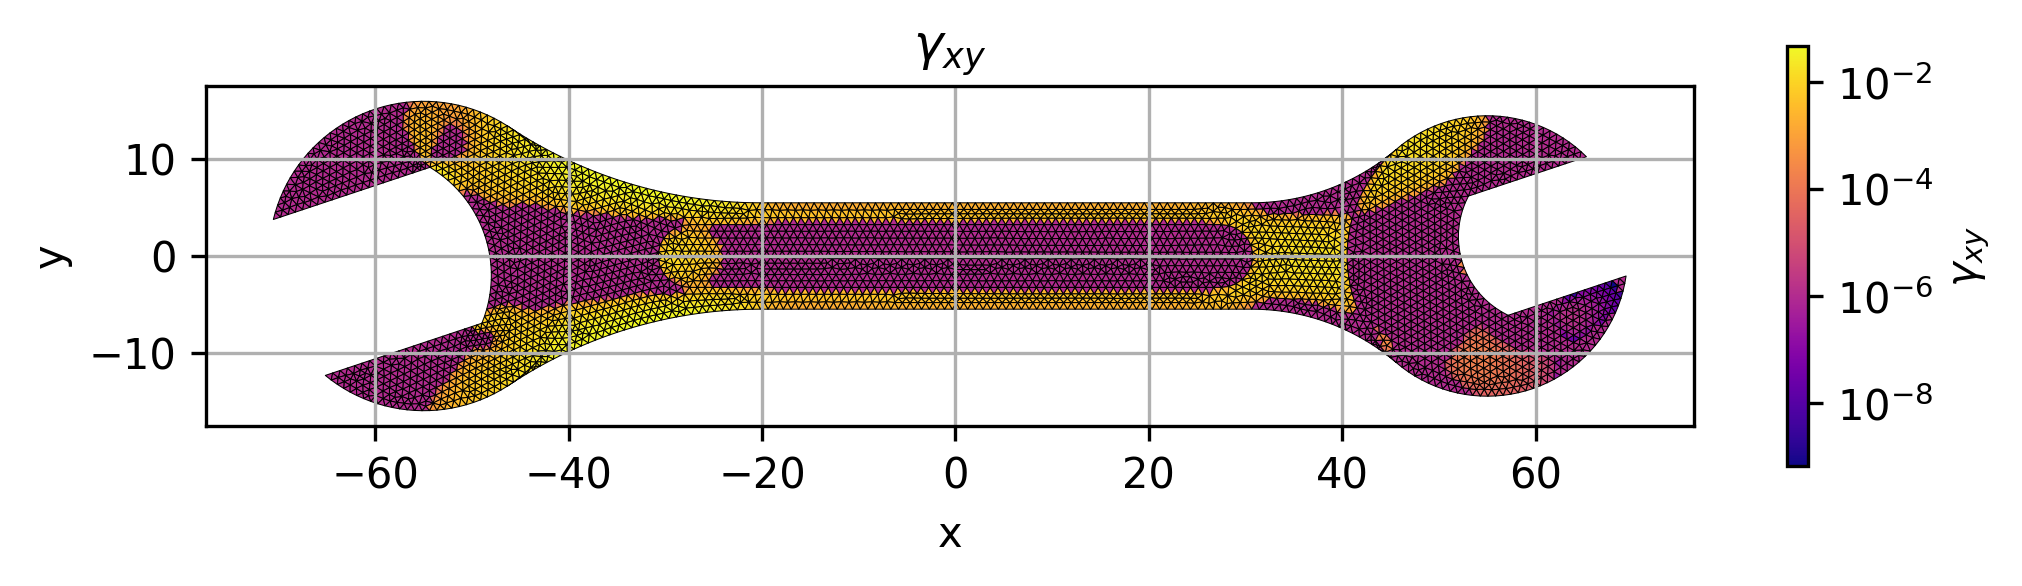
\includegraphics[width=\textwidth]{GRAFICOS/Case a - gamma_xy_per_element.png}
      \caption{Caption}
      \label{fig:von_mises}
    \end{subfigure}
    \caption{Caption}
    \label{fig:analisis_estructural}
  \end{figure}

  \begin{figure}[H]
    \centering
    \begin{subfigure}[t]{0.49\textwidth}
      \centering
      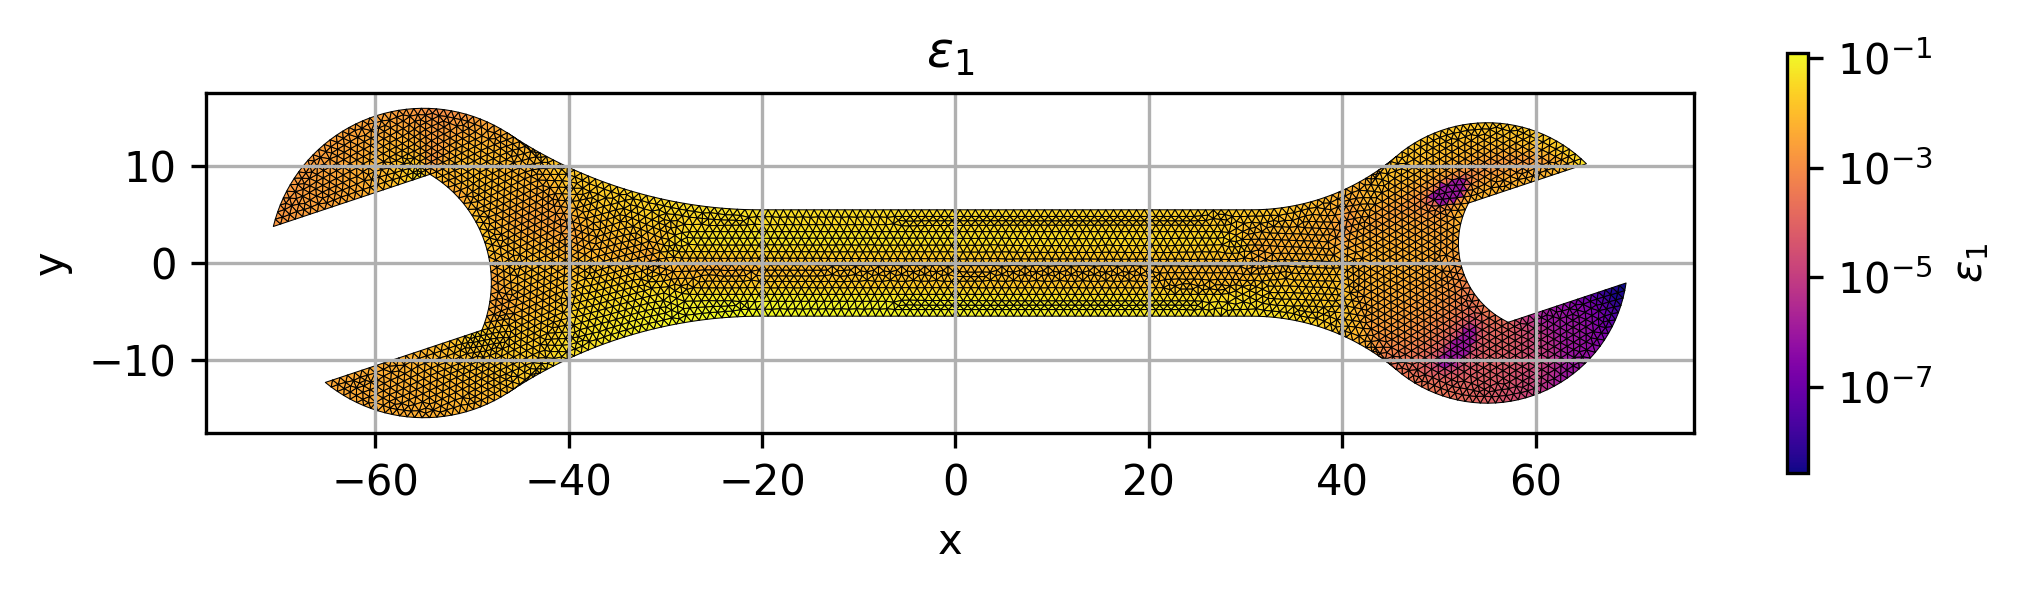
\includegraphics[width=\textwidth]{GRAFICOS/Case a - epsilon_1_per_element.png}
      \caption{Caption}
      \label{fig:deformada_reacciones}
    \end{subfigure}
    \hfill
    \begin{subfigure}[t]{0.49\textwidth}
      \centering
      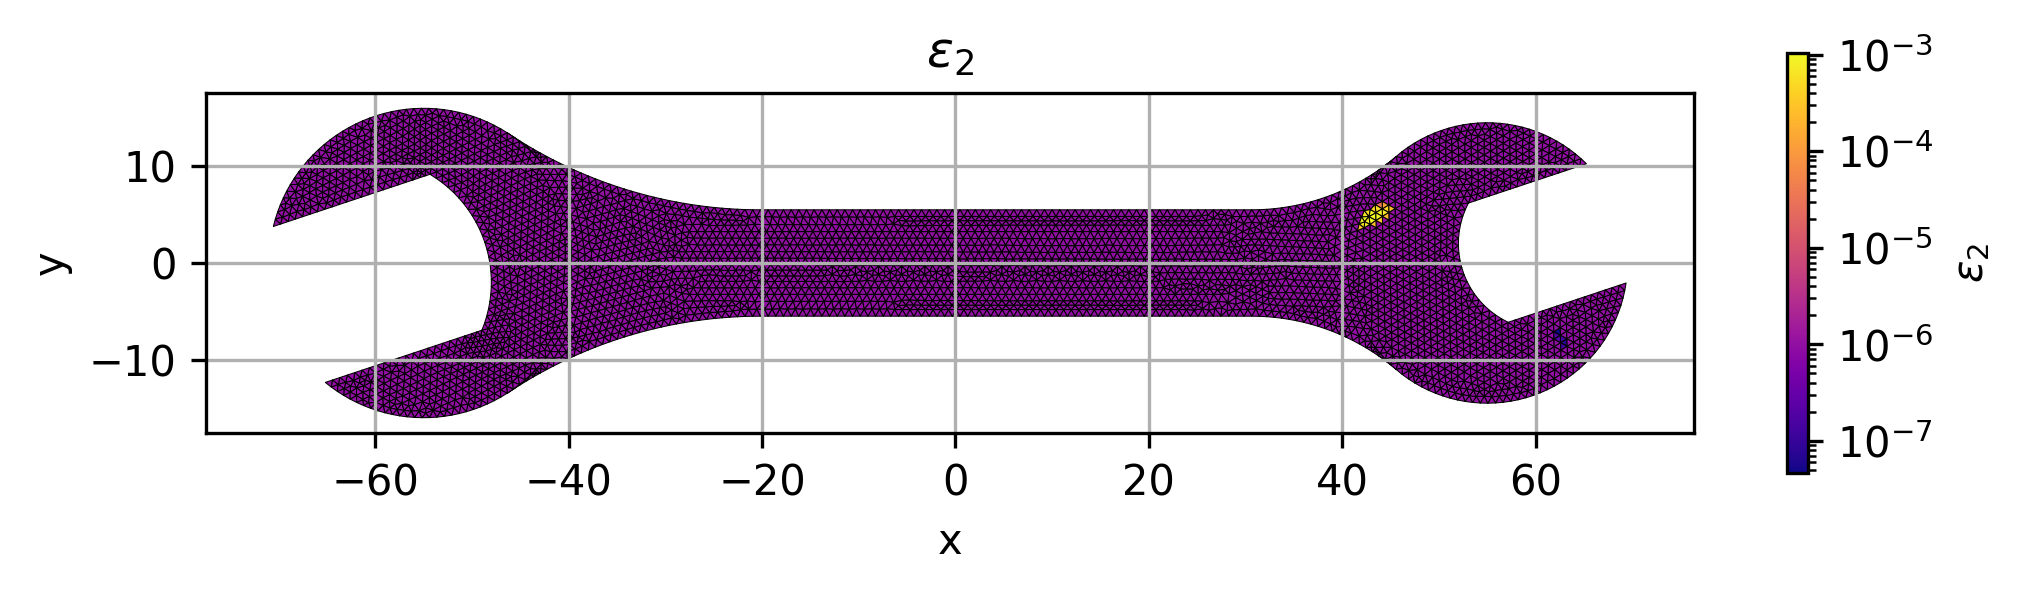
\includegraphics[width=\textwidth]{GRAFICOS/Case a - epsilon_2_per_element.png}
      \caption{Caption}
      \label{fig:von_mises}
    \end{subfigure}
    \caption{Caption}
    \label{fig:analisis_estructural}
  \end{figure}
  
  \begin{figure}[H]
    \centering
    \begin{subfigure}[t]{0.49\textwidth}
      \centering
      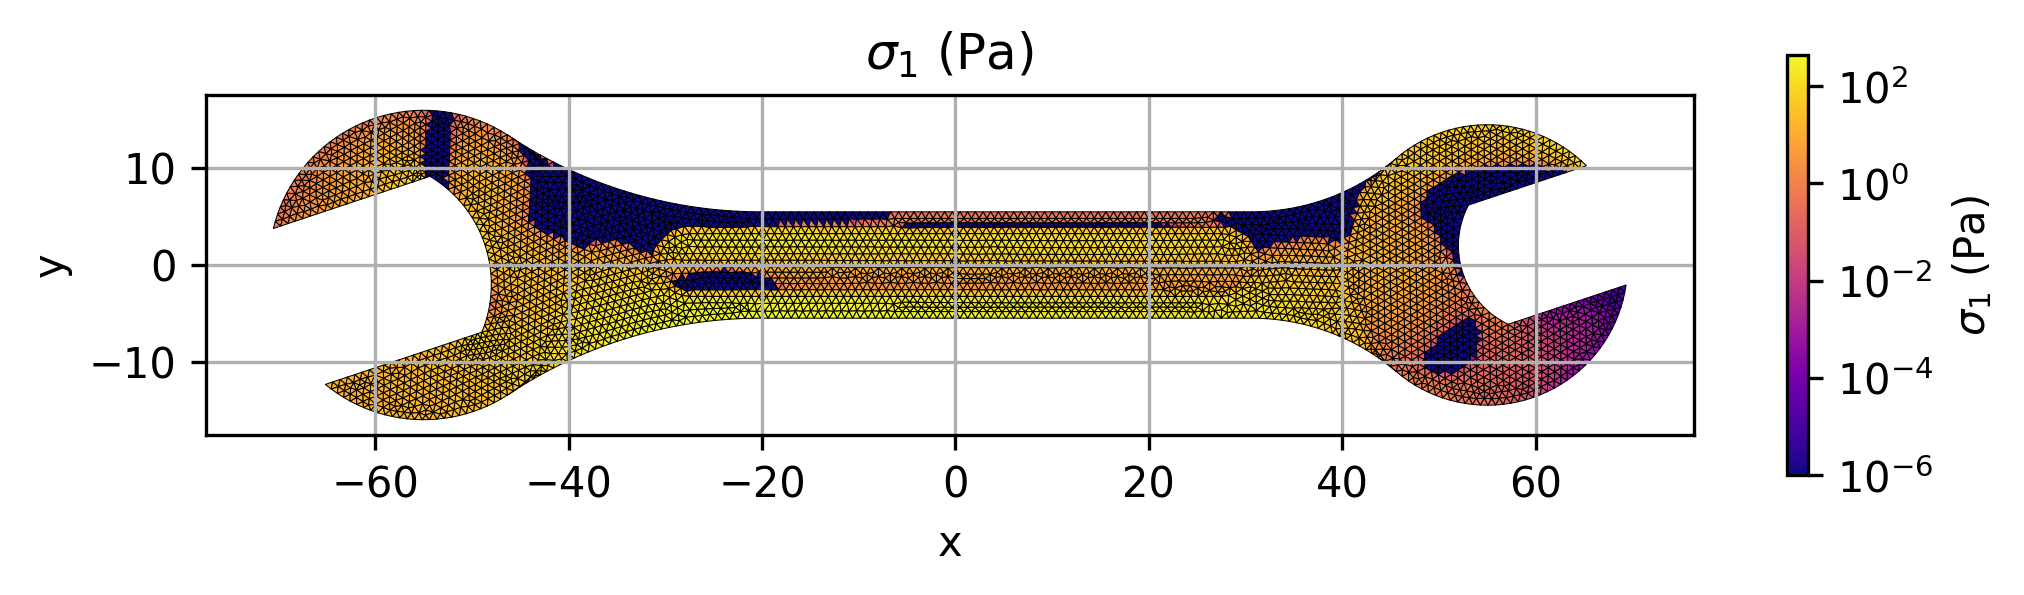
\includegraphics[width=\textwidth]{GRAFICOS/Case a - sigma_1_per_element.png}
      \caption{Caption}
      \label{fig:deformada_reacciones}
    \end{subfigure}
    \hfill
    \begin{subfigure}[t]{0.49\textwidth}
      \centering
      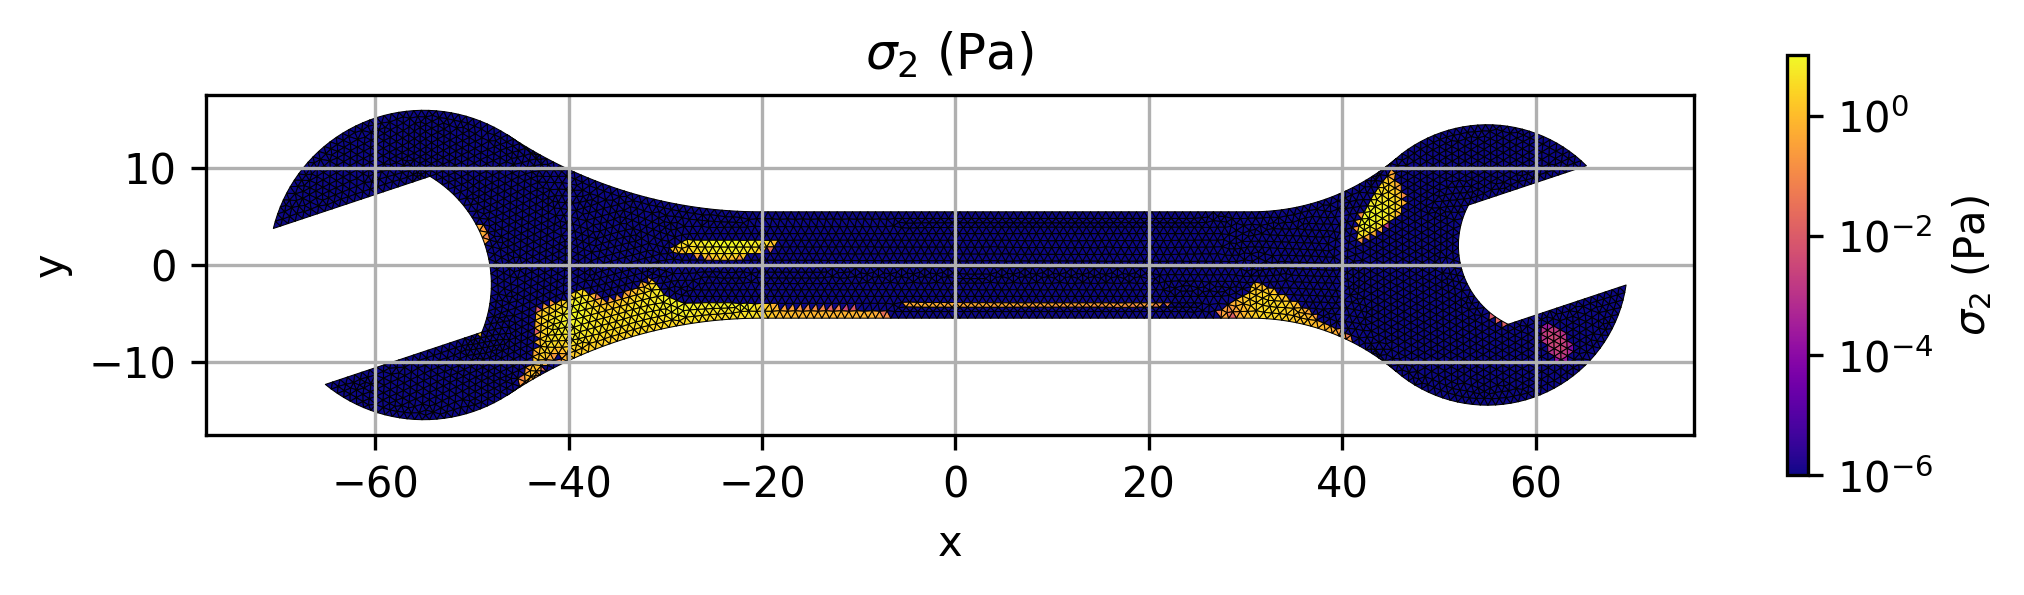
\includegraphics[width=\textwidth]{GRAFICOS/Case a - sigma_2_per_element.png}
      \caption{Caption}
      \label{fig:von_mises}
    \end{subfigure}
    \caption{Caption}
    \label{fig:analisis_estructural}
  \end{figure}

\subsection{Case B}

\begin{figure}[H]
    \centering
    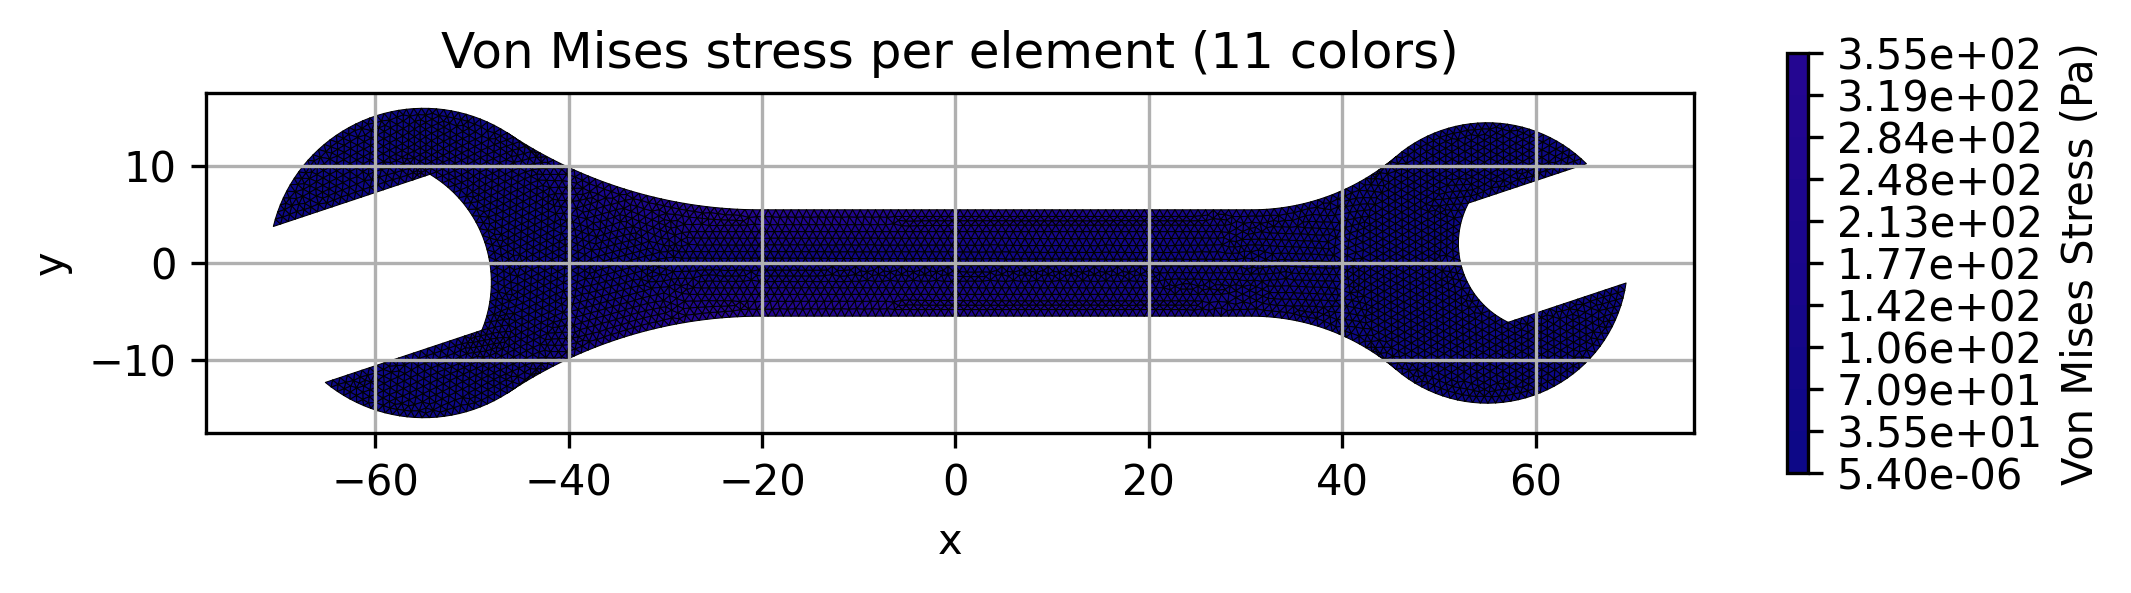
\includegraphics[width=0.8\textwidth]{GRAFICOS/Case b_von_mises_per_element_11_colors.png}
    \caption{Caption}
    \label{fig:strain}
  \end{figure}

  \begin{figure}[H]
    \centering
    \begin{subfigure}[t]{0.49\textwidth}
      \centering
      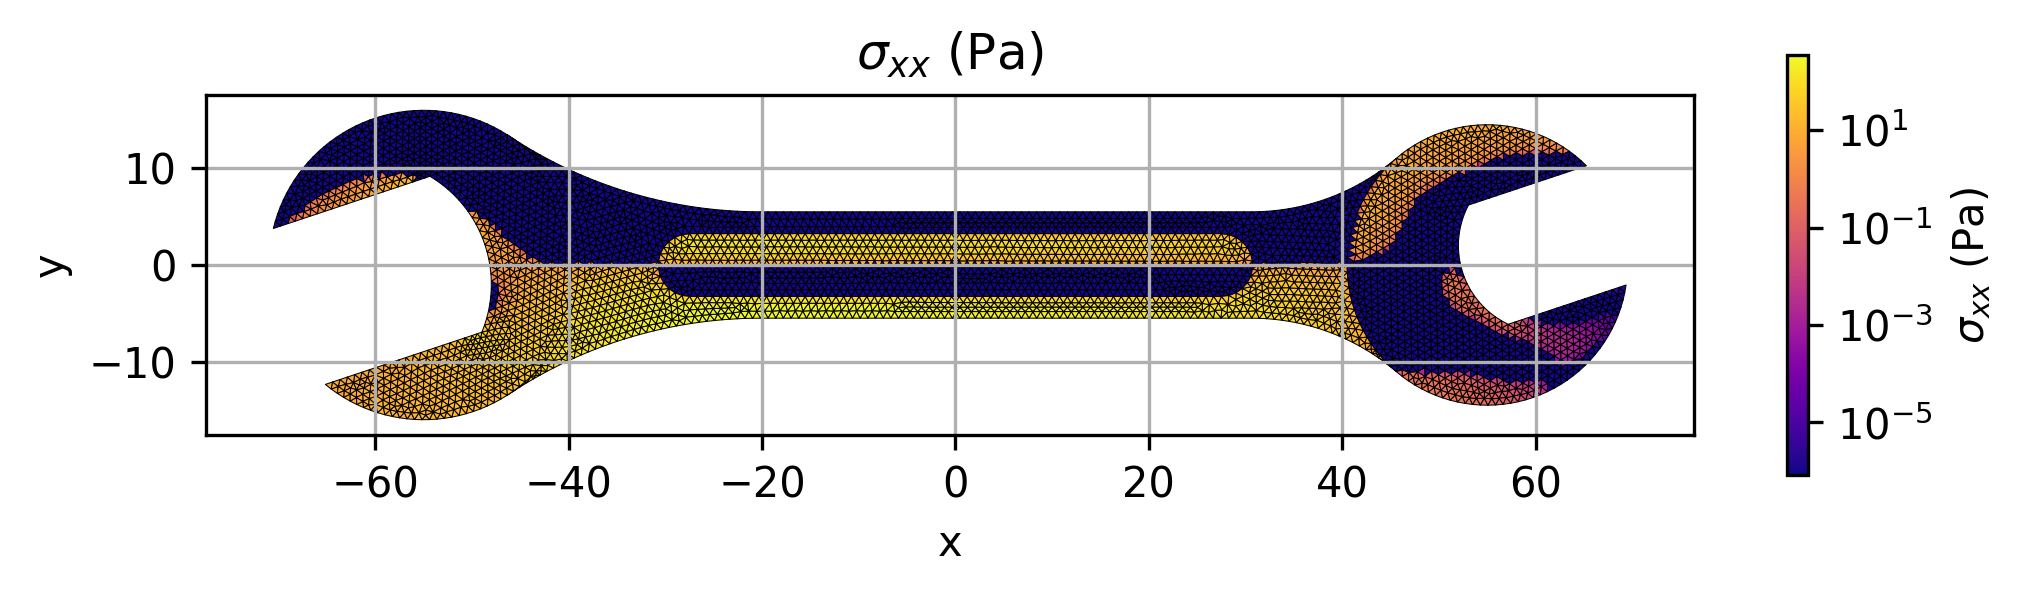
\includegraphics[width=\textwidth]{GRAFICOS/Case b - sigma_xx_per_element.png}
      \caption{Caption}
      \label{fig:deformada_reacciones}
    \end{subfigure}
    \hfill
    \begin{subfigure}[t]{0.49\textwidth}
      \centering
      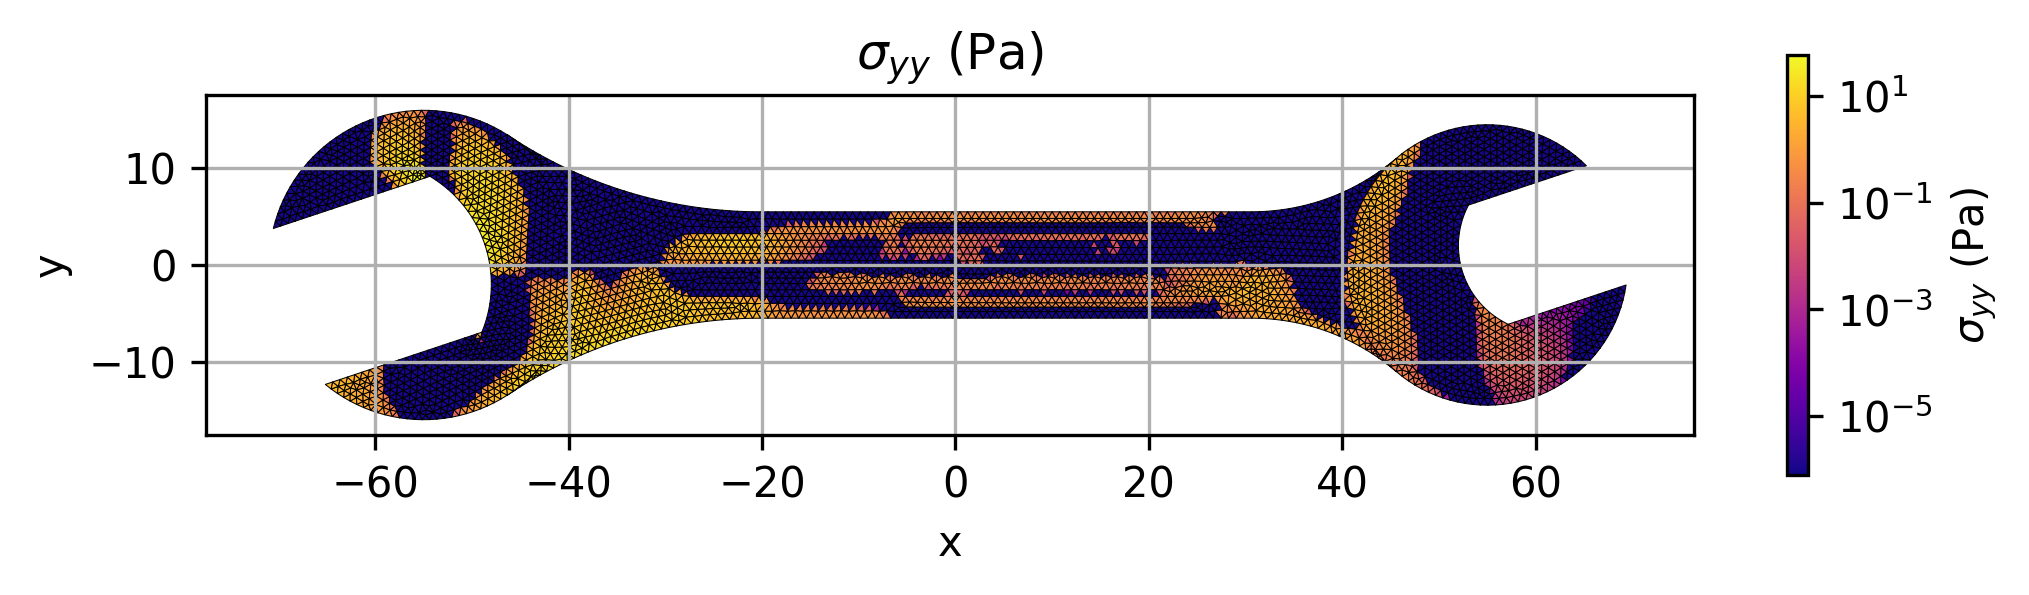
\includegraphics[width=\textwidth]{GRAFICOS/Case b - sigma_yy_per_element.png}
      \caption{Caption}
      \label{fig:von_mises}
    \end{subfigure}
    \caption{Caption}
    \label{fig:analisis_estructural}
  \end{figure}

  \begin{figure}[H]
    \centering
    \begin{subfigure}[t]{0.49\textwidth}
      \centering
      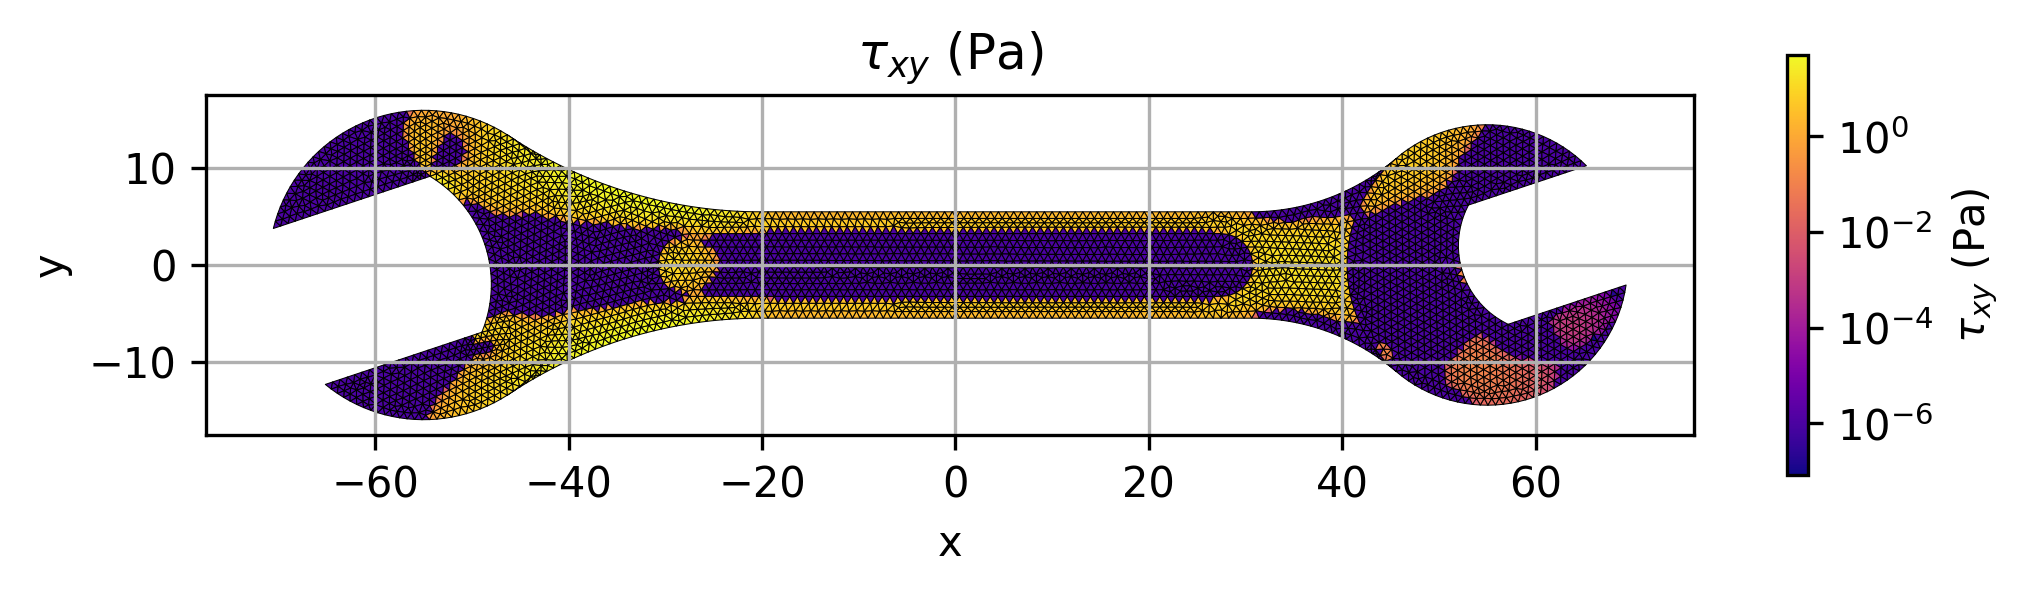
\includegraphics[width=\textwidth]{GRAFICOS/Case b - tau_xy_per_element.png}
      \caption{Caption}
      \label{fig:deformada_reacciones}
    \end{subfigure}

    \hfill

    \begin{subfigure}[t]{0.49\textwidth}
      \centering
      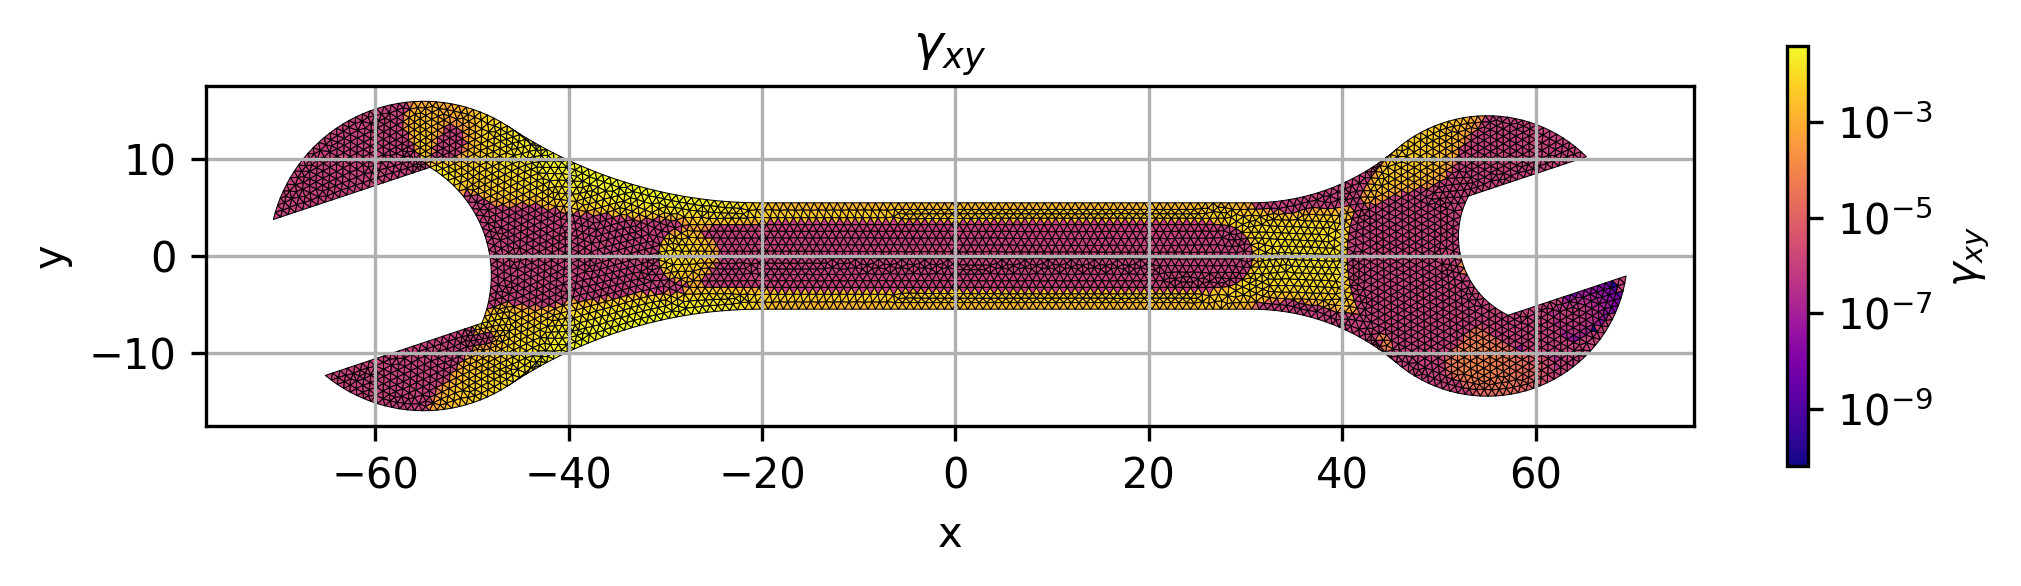
\includegraphics[width=\textwidth]{GRAFICOS/Case b - gamma_xy_per_element.png}
      \caption{Caption}
      \label{fig:von_mises}
    \end{subfigure}
    \caption{Caption}
    \label{fig:analisis_estructural}
  \end{figure}

    \begin{figure}[H]
        \centering
        \begin{subfigure}[t]{0.49\textwidth}
        \centering
        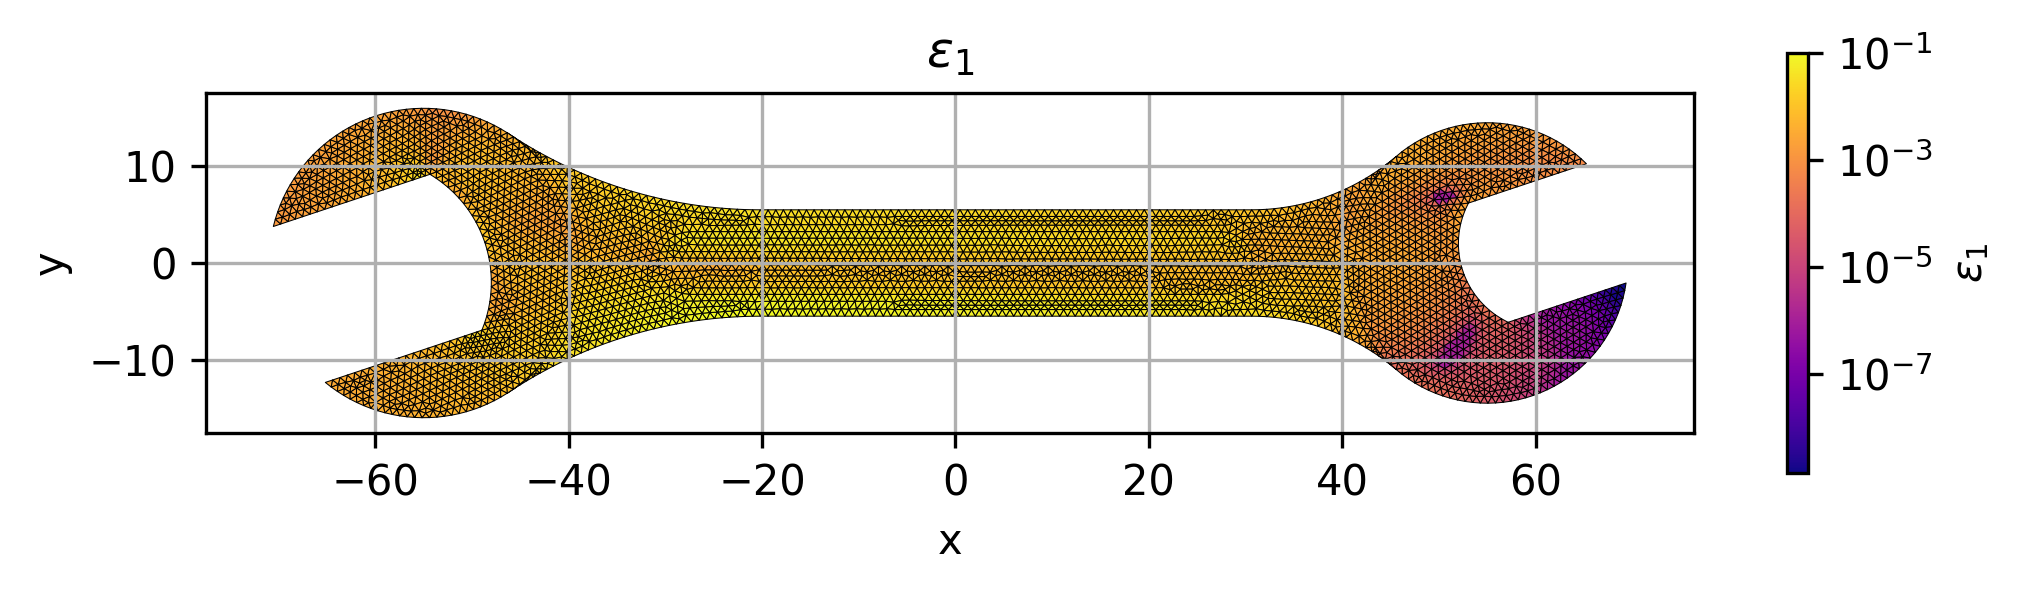
\includegraphics[width=\textwidth]{GRAFICOS/Case b - epsilon_1_per_element.png}
        \caption{Caption}
        \label{fig:deformada_reacciones}
        \end{subfigure}
        \hfill
        \begin{subfigure}[t]{0.49\textwidth}
        \centering
        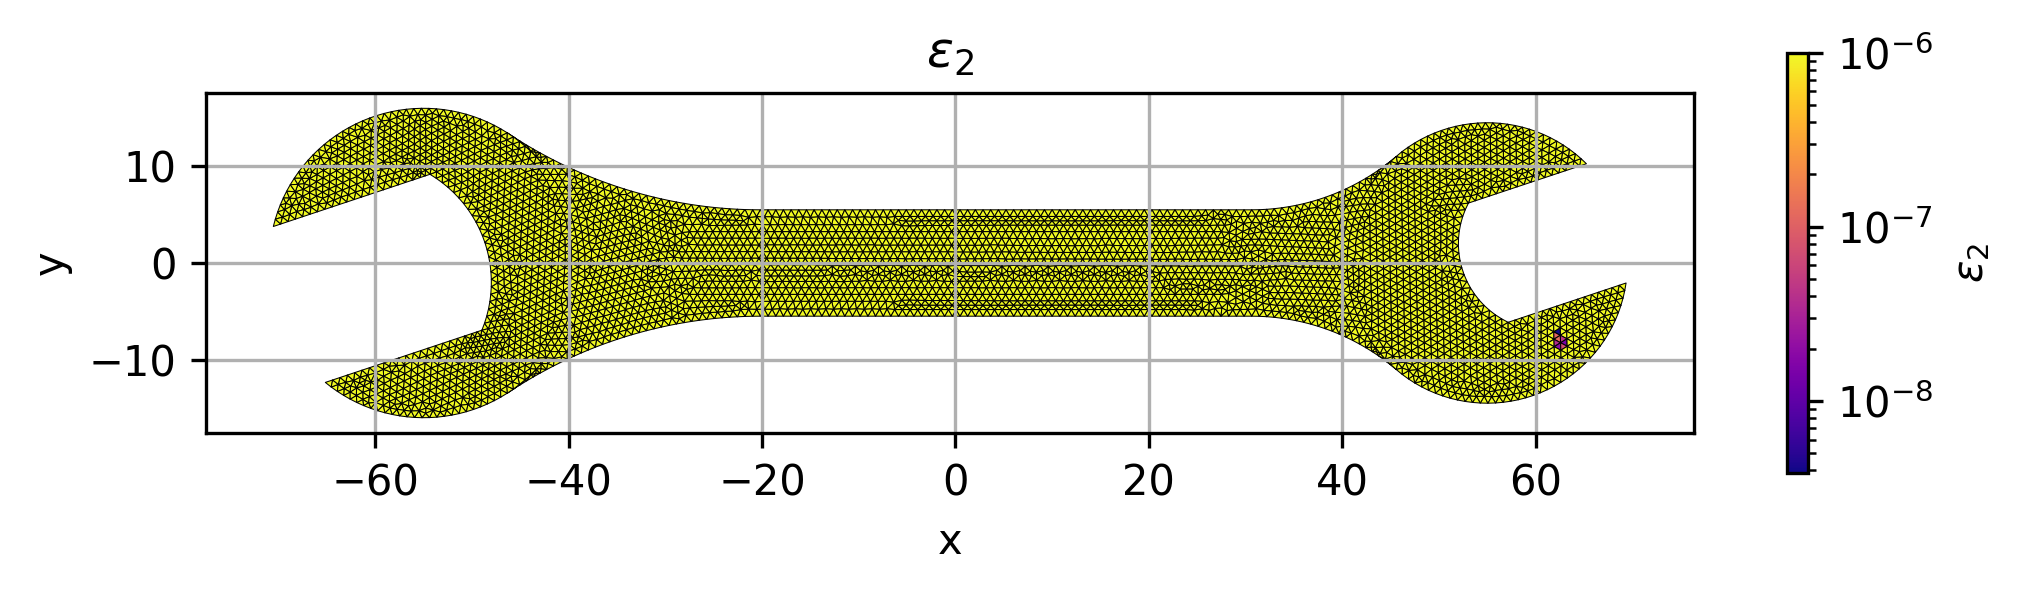
\includegraphics[width=\textwidth]{GRAFICOS/Case b - epsilon_2_per_element.png}
        \caption{Caption}
        \label{fig:von_mises}
        \end{subfigure}
        \caption{Caption}
        \label{fig:analisis_estructural}
    \end{figure}

    \begin{figure}[H]
        \centering
        \begin{subfigure}[t]{0.49\textwidth}
        \centering
        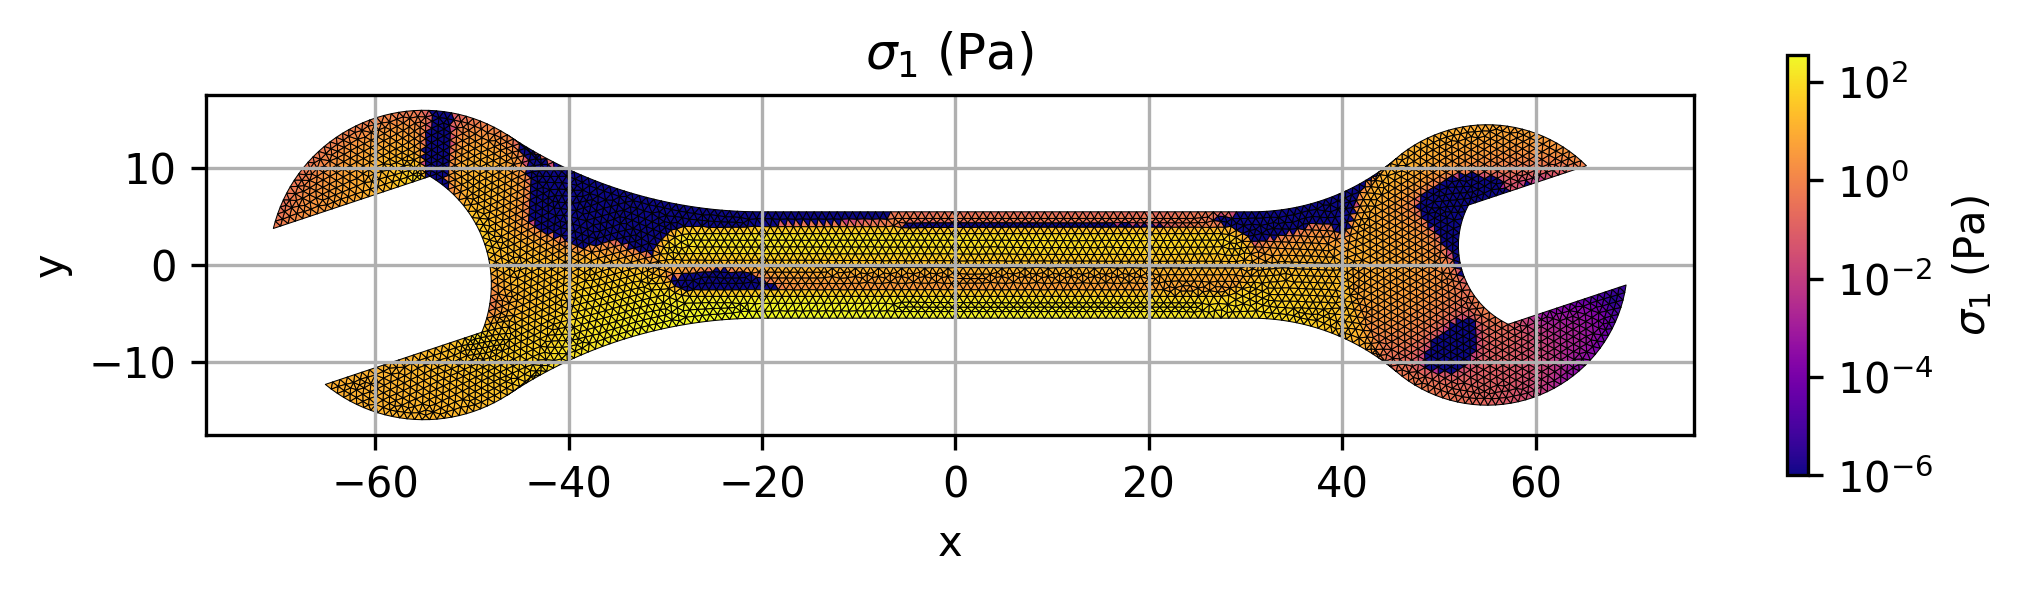
\includegraphics[width=\textwidth]{GRAFICOS/Case b - sigma_1_per_element.png}
        \caption{Caption}
        \label{fig:deformada_reacciones}
        \end{subfigure}
        \hfill
        \begin{subfigure}[t]{0.49\textwidth}
        \centering
        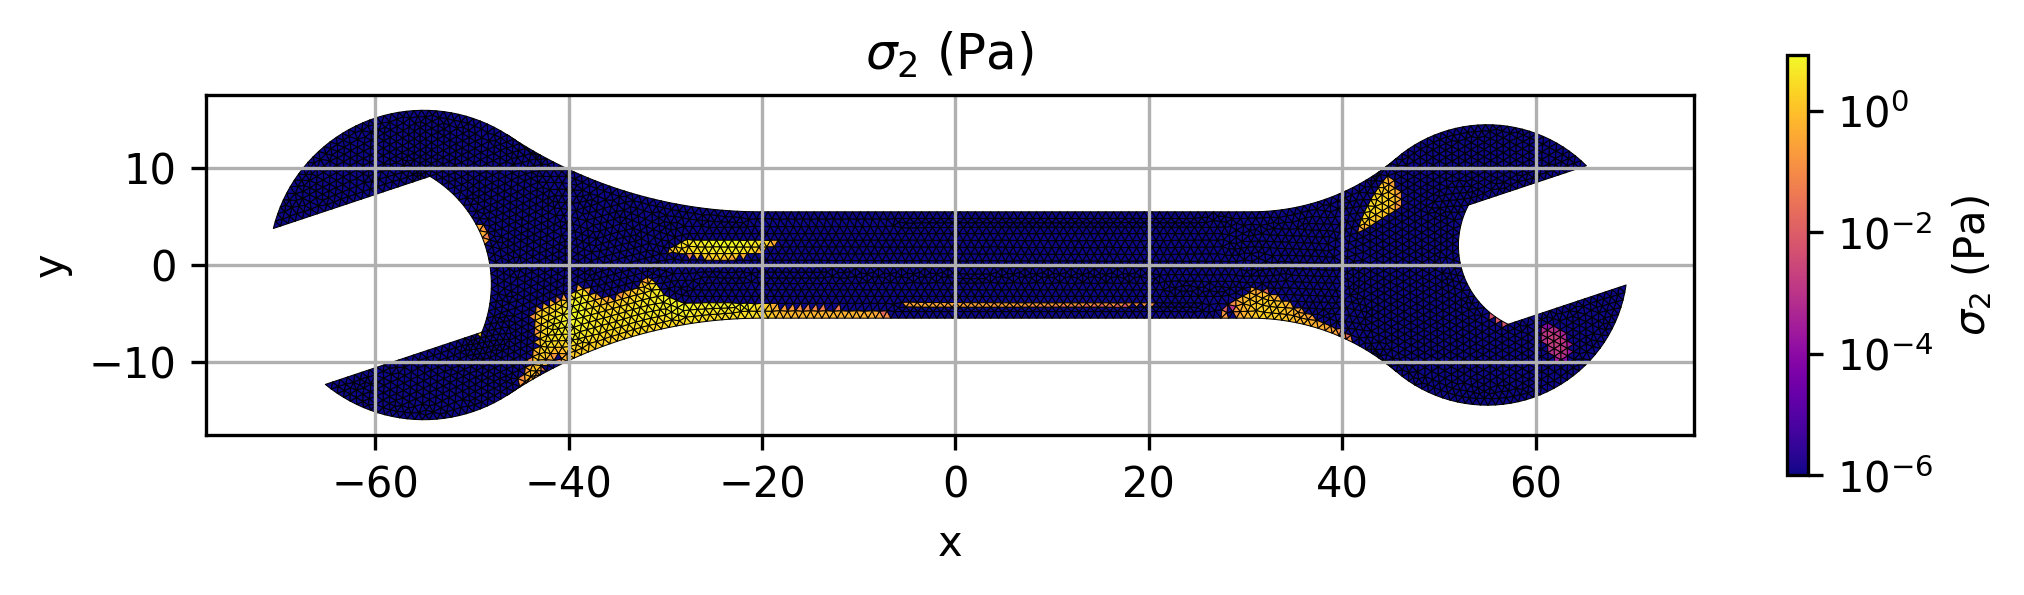
\includegraphics[width=\textwidth]{GRAFICOS/Case b - sigma_2_per_element.png}
        \caption{Caption}
        \label{fig:von_mises}
        \end{subfigure}
        \caption{Caption}
        \label{fig:analisis_estructural}
    \end{figure}

\subsection{Case C}

\begin{figure}[H]
    \centering
    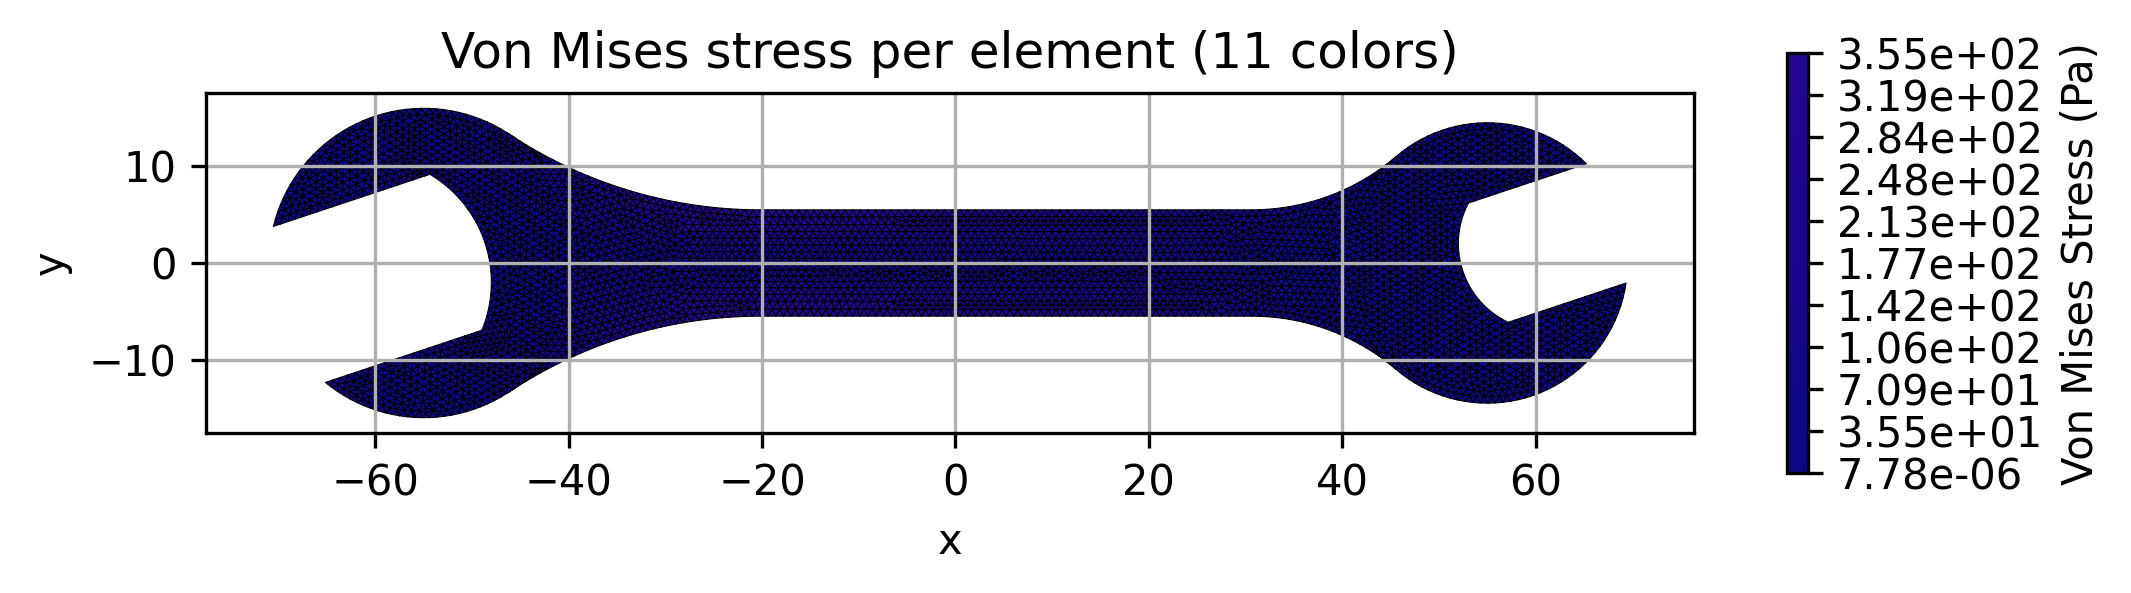
\includegraphics[width=0.8\textwidth]{GRAFICOS/Case c_von_mises_per_element_11_colors.png}
    \caption{Caption}
    \label{fig:strain}
  \end{figure}

  \begin{figure}[H]
    \centering
    \begin{subfigure}[t]{0.49\textwidth}
      \centering
      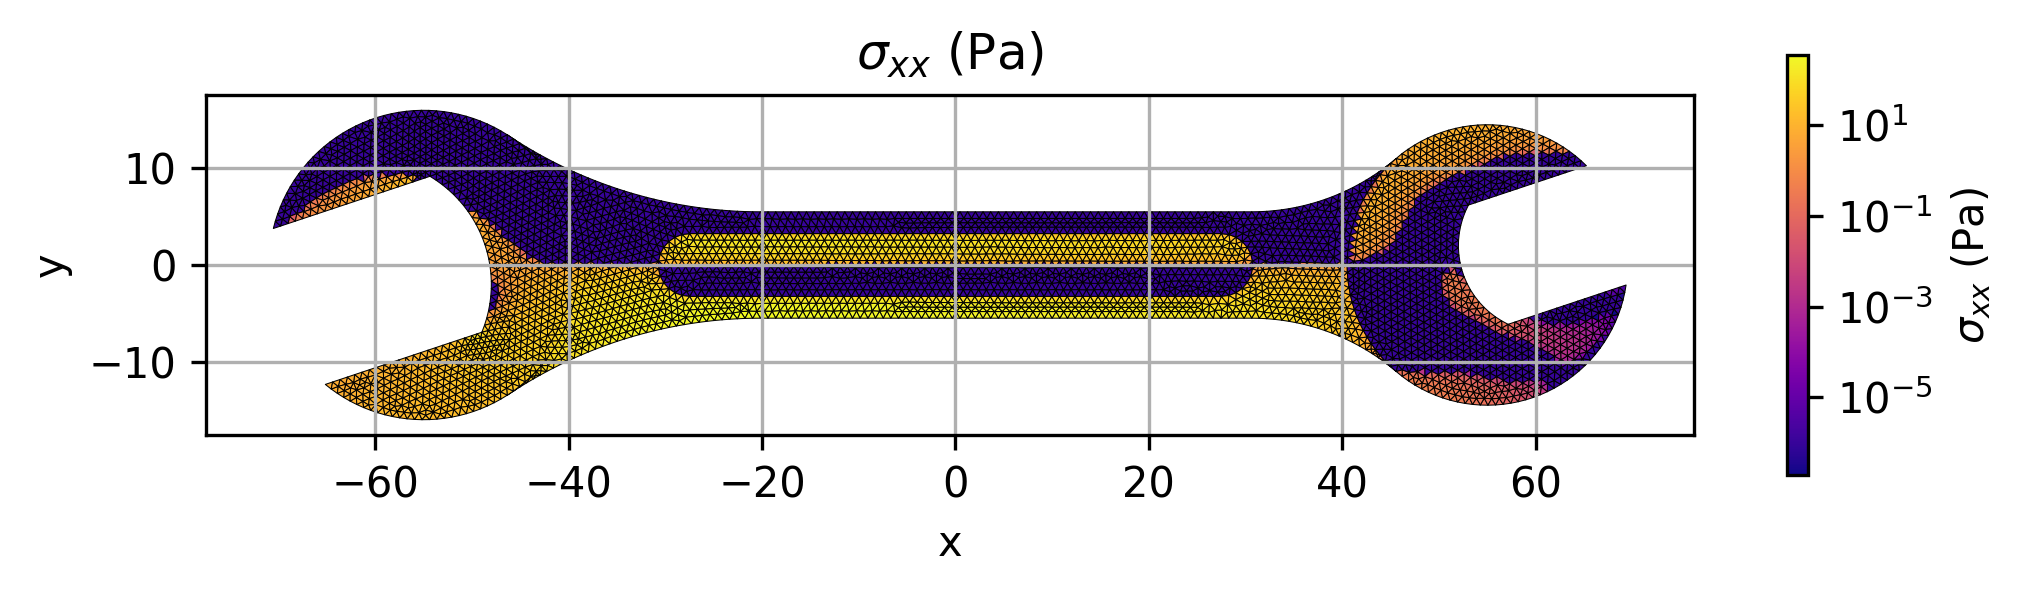
\includegraphics[width=\textwidth]{GRAFICOS/Case c - sigma_xx_per_element.png}
      \caption{Caption}
      \label{fig:deformada_reacciones}
    \end{subfigure}
    \hfill
    \begin{subfigure}[t]{0.49\textwidth}
      \centering
      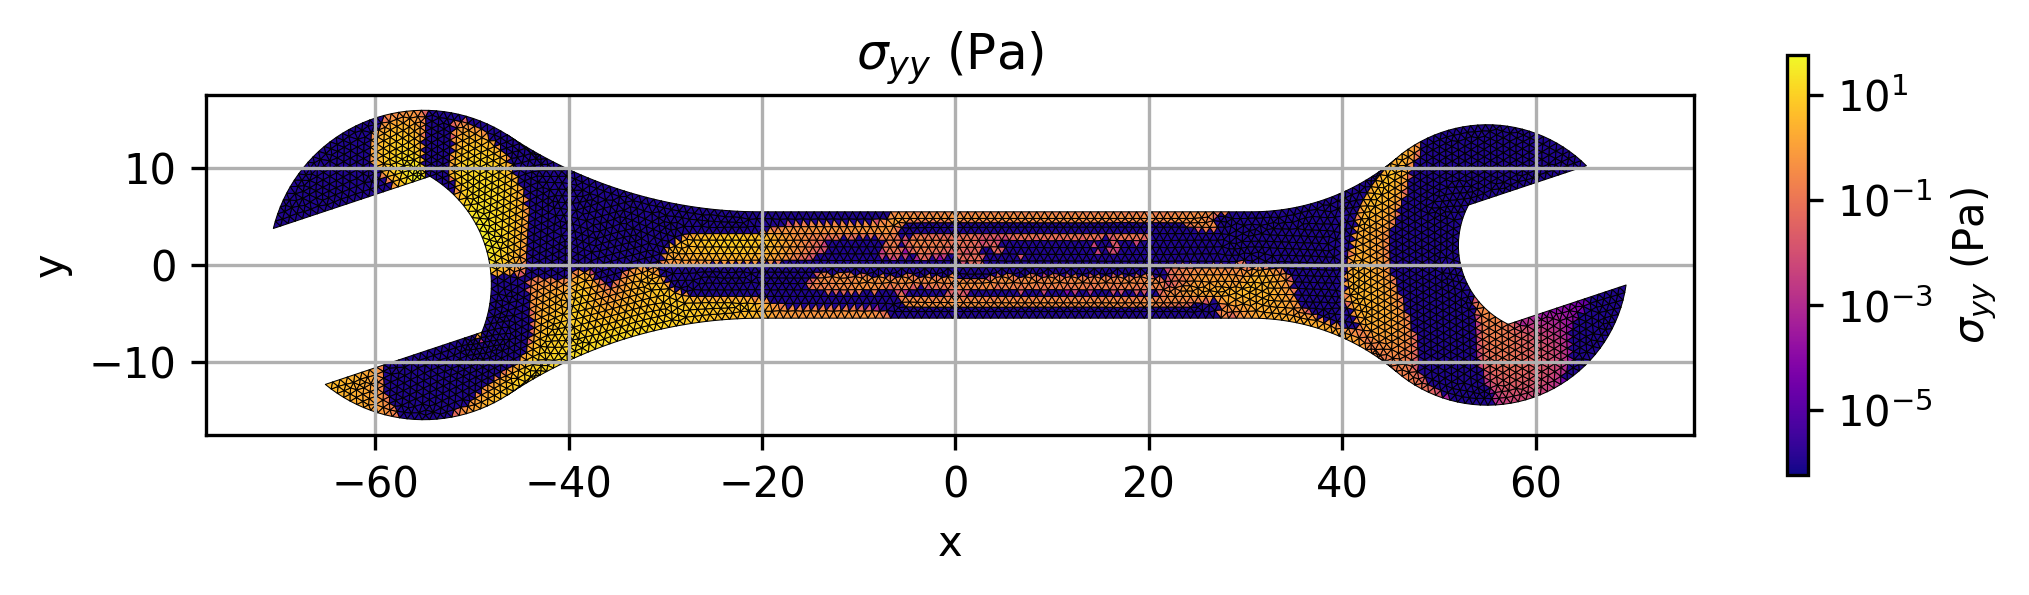
\includegraphics[width=\textwidth]{GRAFICOS/Case c - sigma_yy_per_element.png}
      \caption{Caption}
      \label{fig:von_mises}
    \end{subfigure}
    \caption{Caption}
    \label{fig:analisis_estructural}
  \end{figure}

  \begin{figure}[H]
    \centering
    \begin{subfigure}[t]{0.49\textwidth}
      \centering
      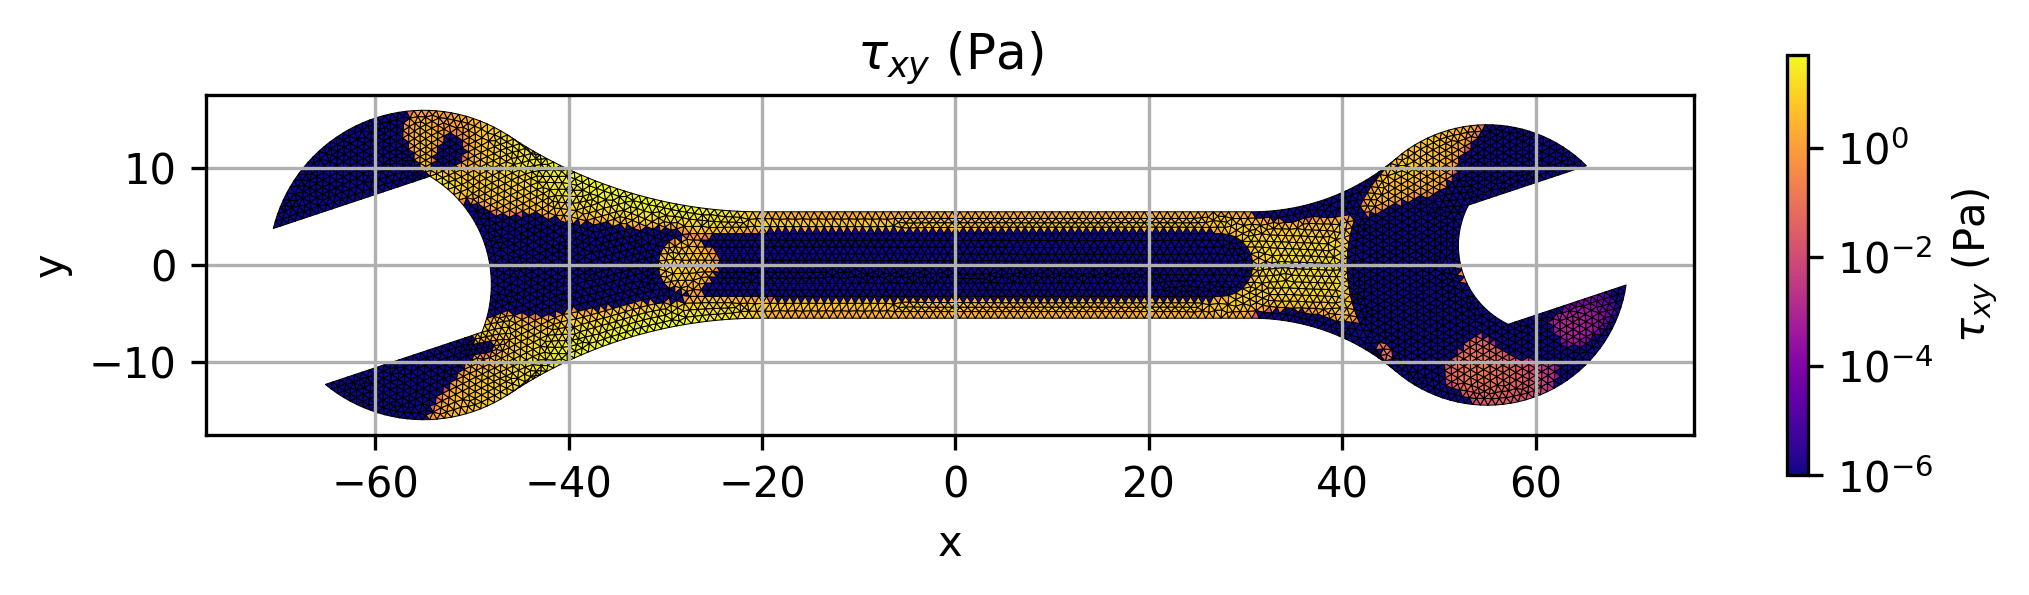
\includegraphics[width=\textwidth]{GRAFICOS/Case c - tau_xy_per_element.png}
      \caption{Caption}
      \label{fig:deformada_reacciones}
    \end{subfigure}

    \hfill

    \begin{subfigure}[t]{0.49\textwidth}
      \centering
      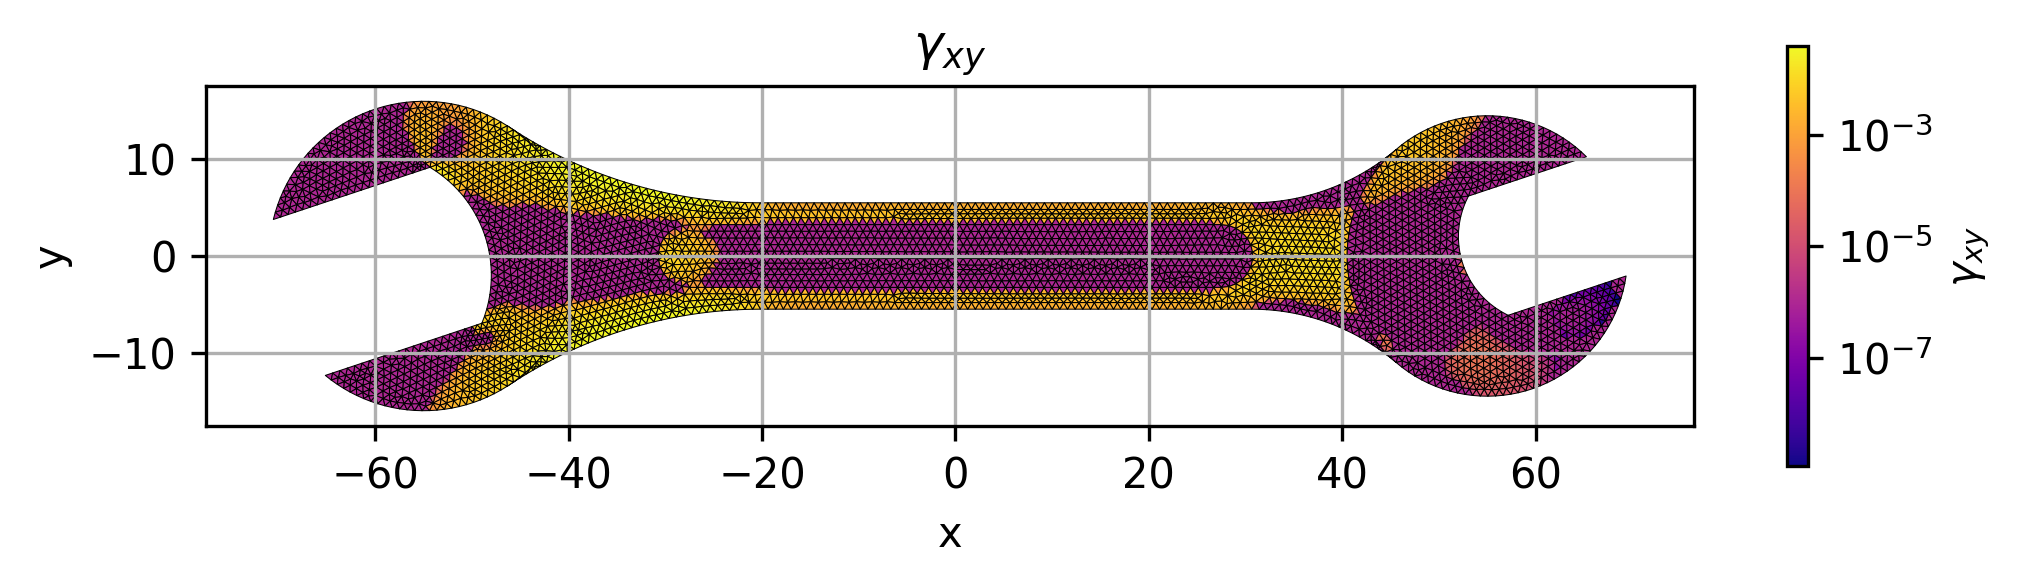
\includegraphics[width=\textwidth]{GRAFICOS/Case c - gamma_xy_per_element.png}
      \caption{Caption}
      \label{fig:von_mises}

    \end{subfigure}
    \caption{Caption}
    \label{fig:analisis_estructural}
    \end{figure}


    \begin{figure}[H]
        \centering
        \begin{subfigure}[t]{0.49\textwidth}
        \centering
        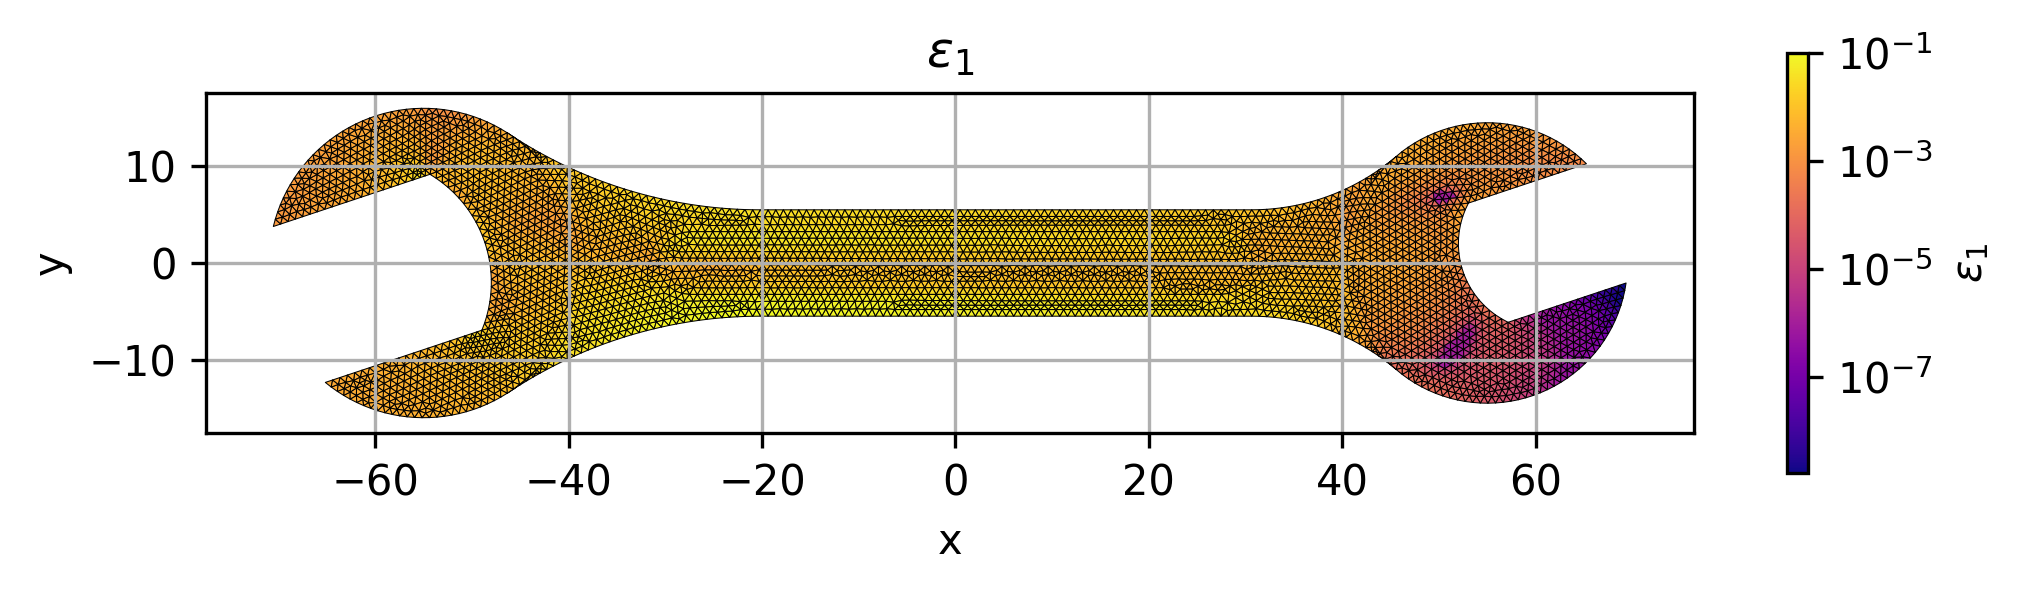
\includegraphics[width=\textwidth]{GRAFICOS/Case c - epsilon_1_per_element.png}
        \caption{Caption}
        \label{fig:deformada_reacciones}
        \end{subfigure}
        \hfill
        \begin{subfigure}[t]{0.49\textwidth}
        \centering
        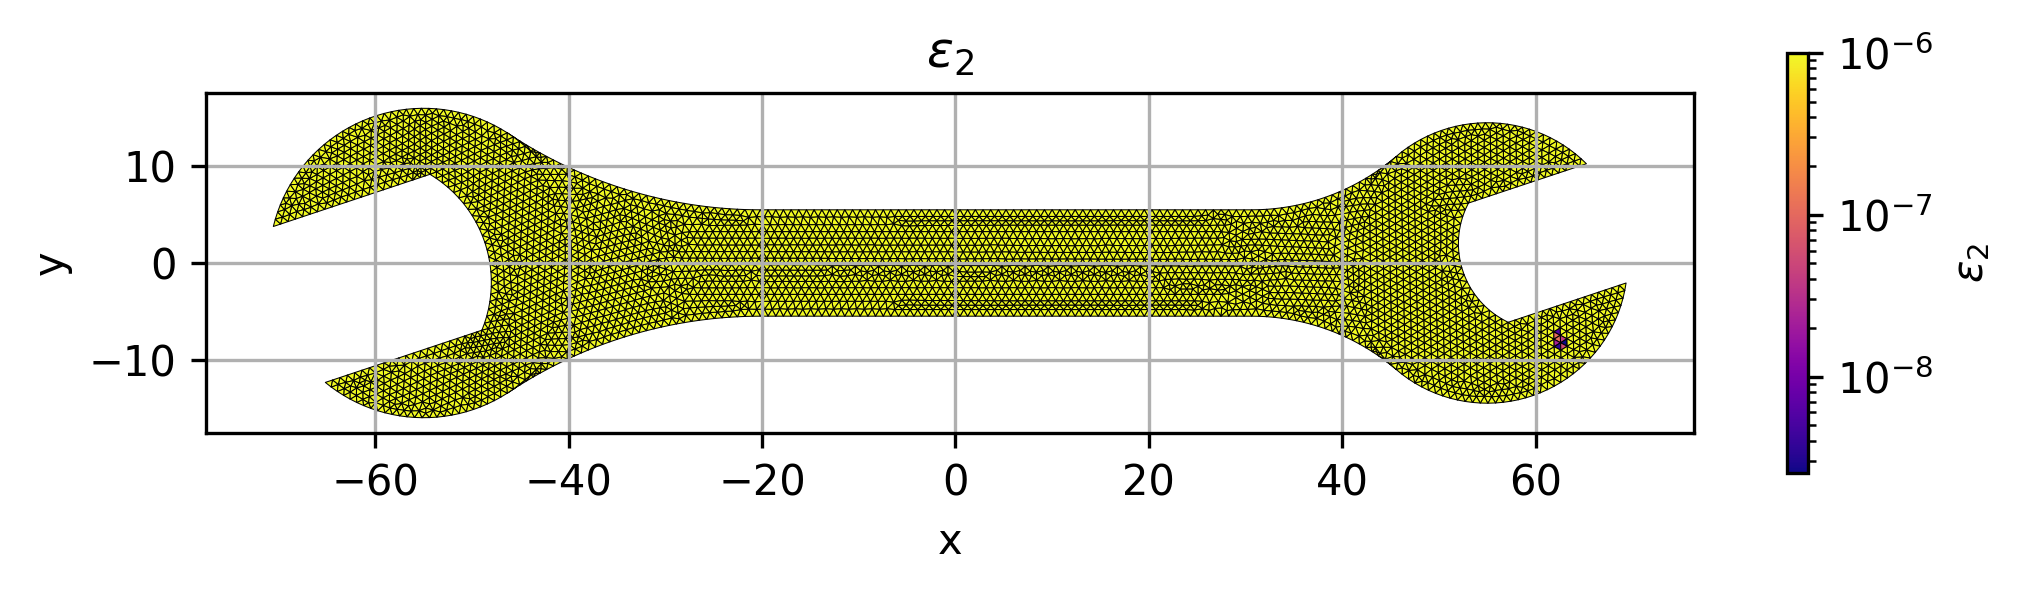
\includegraphics[width=\textwidth]{GRAFICOS/Case c - epsilon_2_per_element.png}
        \caption{Caption}
        \label{fig:von_mises}
        \end{subfigure}
        \caption{Caption}
        \label{fig:analisis_estructural}
    \end{figure}

    \begin{figure}[H]
        \centering
        \begin{subfigure}[t]{0.49\textwidth}
        \centering
        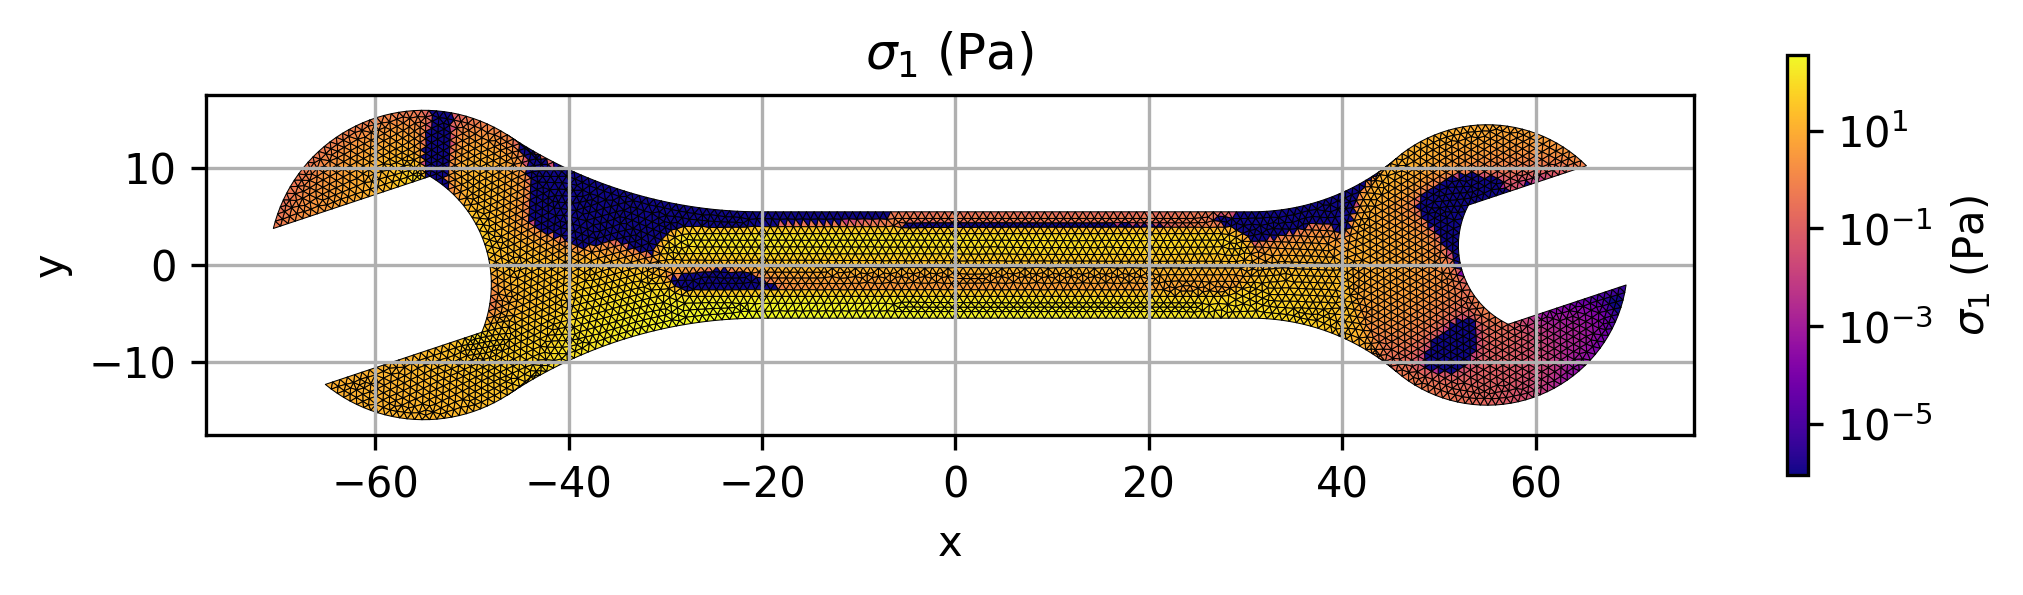
\includegraphics[width=\textwidth]{GRAFICOS/Case c - sigma_1_per_element.png}
        \caption{Caption}
        \label{fig:deformada_reacciones}
        \end{subfigure}
        \hfill
        \begin{subfigure}[t]{0.49\textwidth}
        \centering
        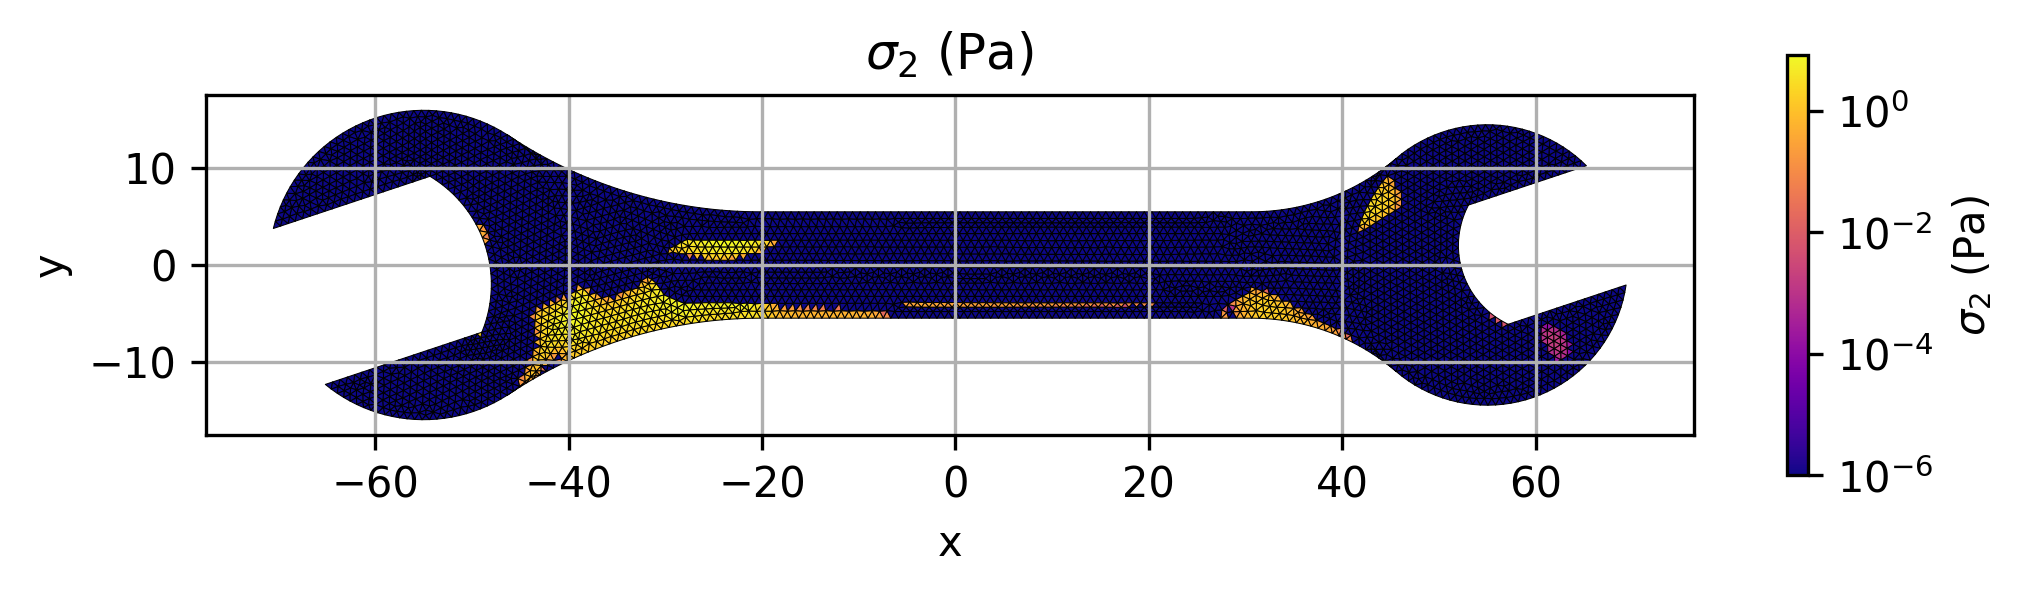
\includegraphics[width=\textwidth]{GRAFICOS/Case c - sigma_2_per_element.png}
        \caption{Caption}
        \label{fig:von_mises}
        \end{subfigure}
        \caption{Caption}
        \label{fig:analisis_estructural}
    \end{figure}

\subsection{Case D}

\begin{figure}[H]
    \centering
    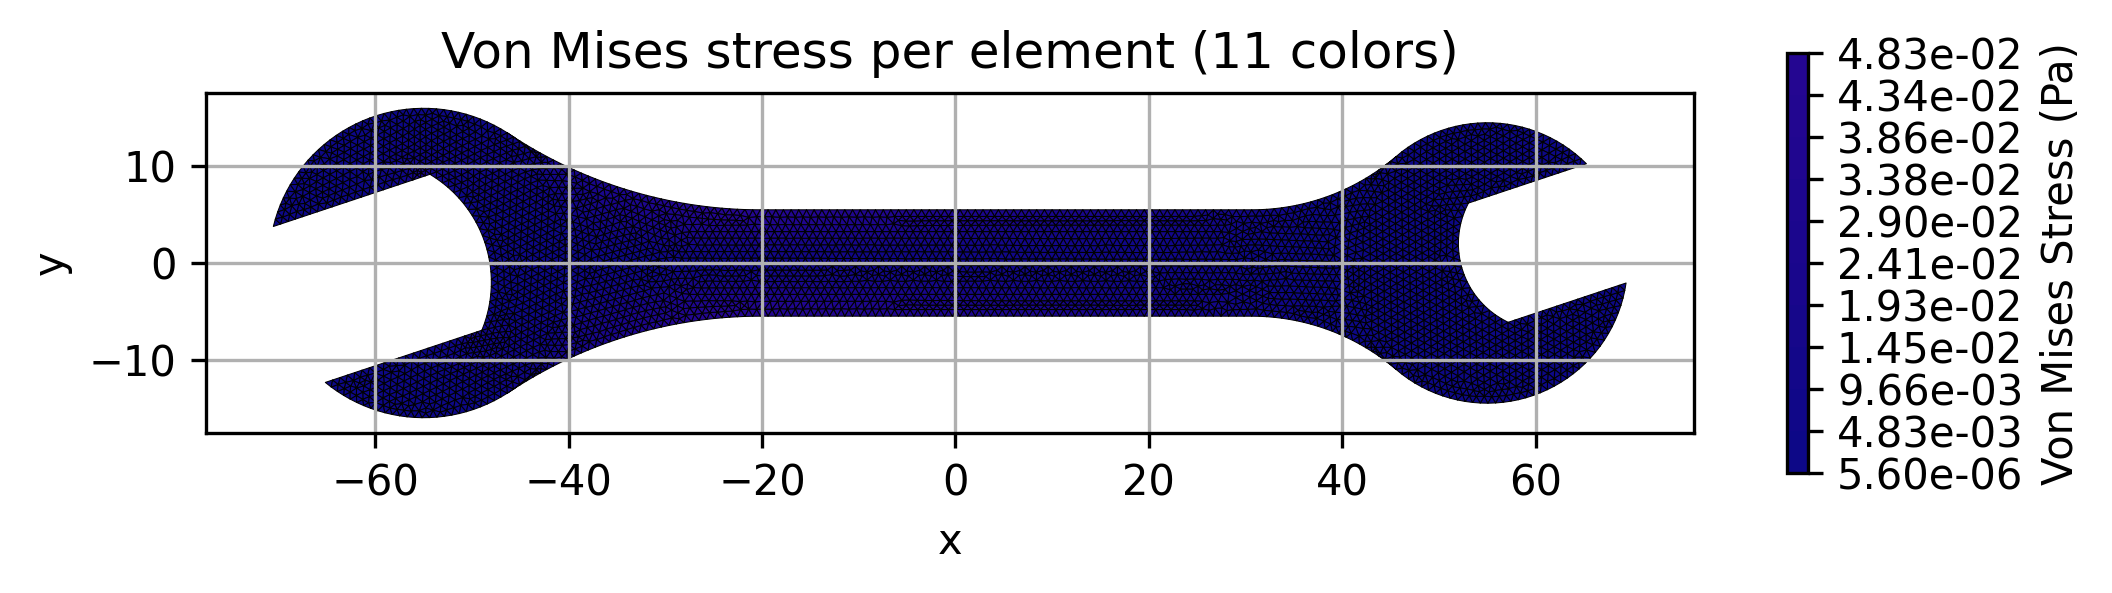
\includegraphics[width=0.8\textwidth]{GRAFICOS/Case d_von_mises_per_element_11_colors.png}
    \caption{Caption}
    \label{fig:strain}
  \end{figure}

  \begin{figure}[H]
    \centering
    \begin{subfigure}[t]{0.49\textwidth}
      \centering
      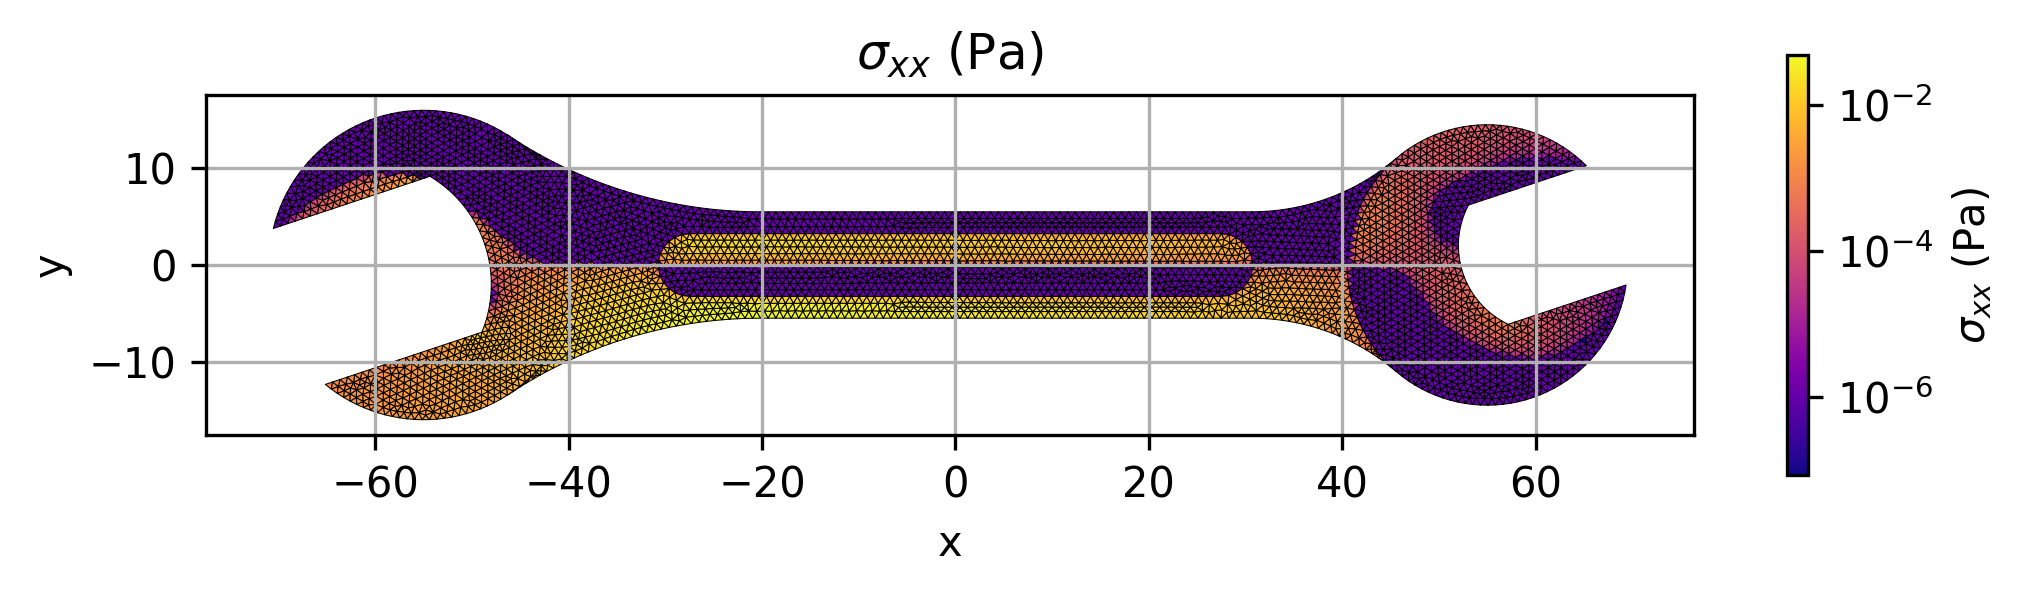
\includegraphics[width=\textwidth]{GRAFICOS/Case d - sigma_xx_per_element.png}
      \caption{Caption}
      \label{fig:deformada_reacciones}
    \end{subfigure}
    \hfill
    \begin{subfigure}[t]{0.49\textwidth}
      \centering
      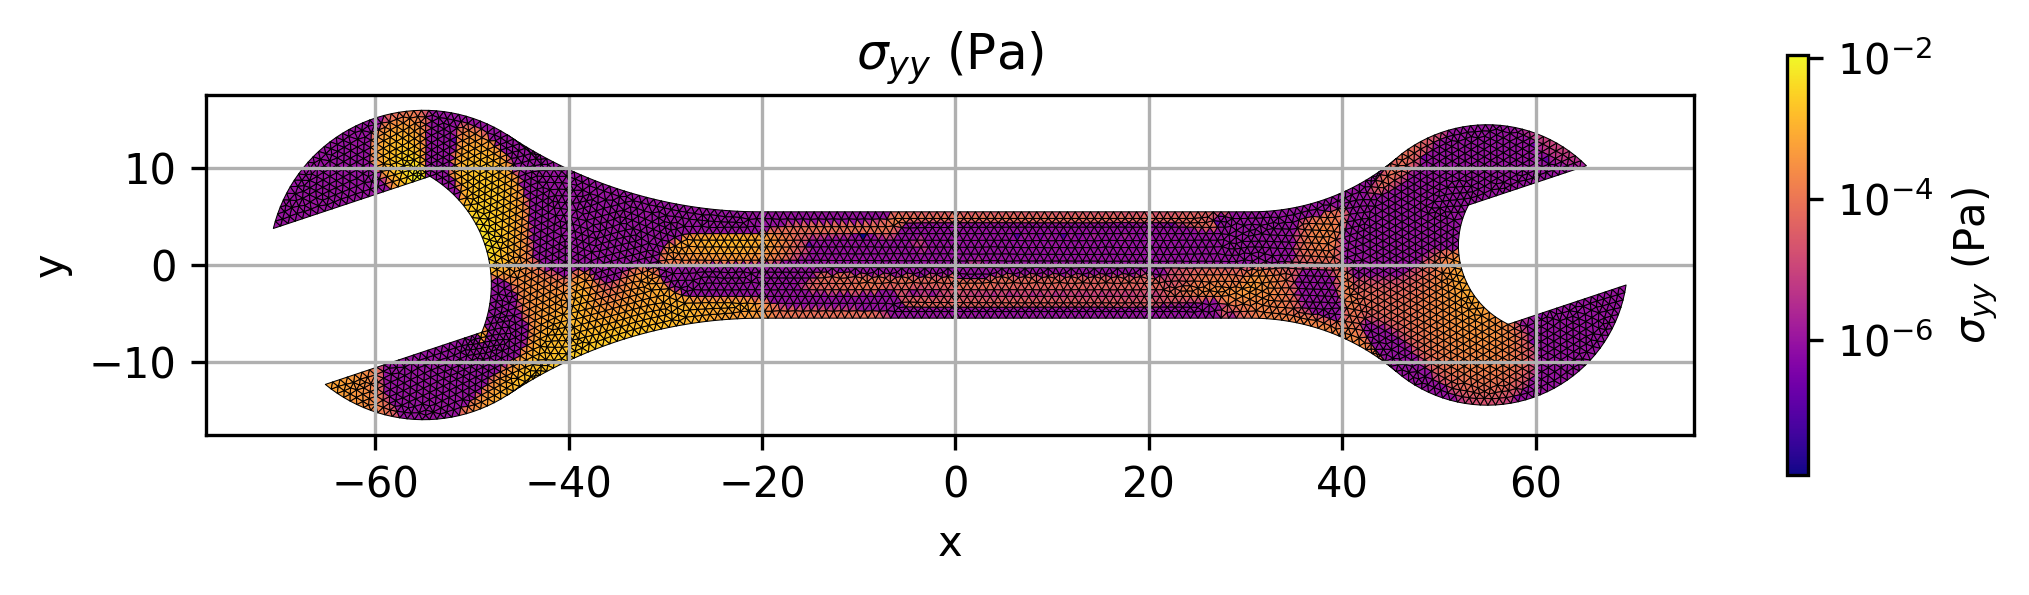
\includegraphics[width=\textwidth]{GRAFICOS/Case d - sigma_yy_per_element.png}
      \caption{Caption}
      \label{fig:von_mises}
    \end{subfigure}
    \caption{Caption}
    \label{fig:analisis_estructural}
  \end{figure}

  \begin{figure}[H]
    \centering
    \begin{subfigure}[t]{0.49\textwidth}
      \centering
      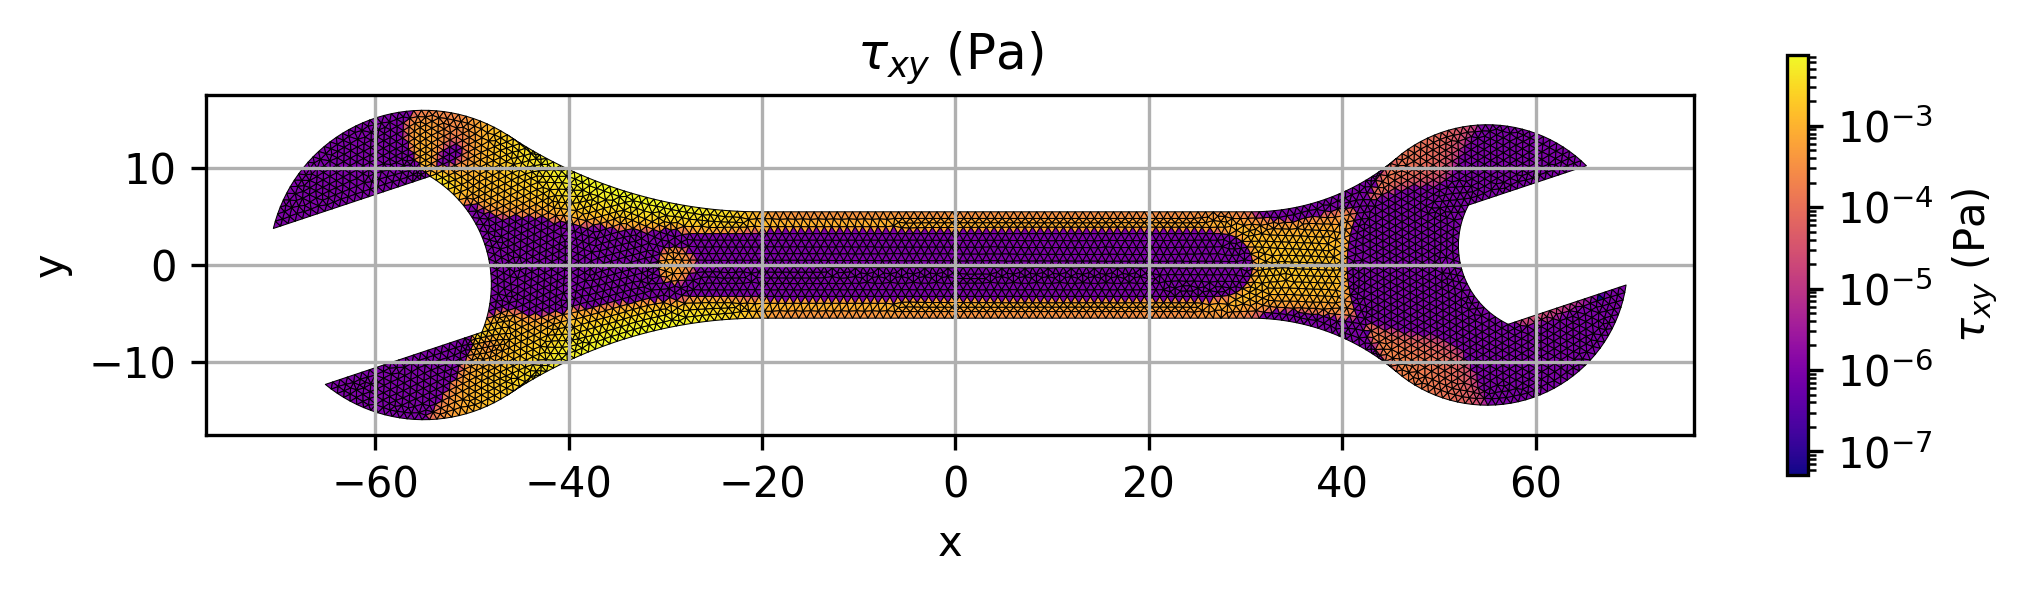
\includegraphics[width=\textwidth]{GRAFICOS/Case d - tau_xy_per_element.png}
      \caption{Caption}
      \label{fig:deformada_reacciones}
    \end{subfigure}
    \hfill
    \begin{subfigure}[t]{0.49\textwidth}
      \centering
      \includegraphics[width=\textwidth]{GRAFICOS/Case d - gamma_xy_per_element.png}
      \caption{Caption}
      \label{fig:von_mises}
    \end{subfigure}
    \caption{Caption}
    \label{fig:analisis_estructural}
    \end{figure}

    \begin{figure}[H]
        \centering
        \begin{subfigure}[t]{0.49\textwidth}
        \centering
        \includegraphics[width=\textwidth]{GRAFICOS/Case d - epsilon_1_per_element.png}
        \caption{Caption}
        \label{fig:deformada_reacciones}
        \end{subfigure}
        \hfill
        \begin{subfigure}[t]{0.49\textwidth}
        \centering
        \includegraphics[width=\textwidth]{GRAFICOS/Case d - epsilon_2_per_element.png}
        \caption{Caption}
        \label{fig:von_mises}
        \end{subfigure}
        \caption{Caption}
        \label{fig:analisis_estructural}
    \end{figure}

    \begin{figure}[H]
        \centering
        \begin{subfigure}[t]{0.49\textwidth}
        \centering
        \includegraphics[width=\textwidth]{GRAFICOS/Case d - sigma_1_per_element.png}
        \caption{Caption}
        \label{fig:deformada_reacciones}
        \end{subfigure}
        \hfill
        \begin{subfigure}[t]{0.49\textwidth}
        \centering
        \includegraphics[width=\textwidth]{GRAFICOS/Case d - sigma_2_per_element.png}
        \caption{Caption}
        \label{fig:von_mises}
        \end{subfigure}
        \caption{Caption}
        \label{fig:analisis_estructural}
    \end{figure}
  

\renewcommand{\refname}{References}
\bibliographystyle{plain}
\bibliography{ref}

\end{document}